\documentclass{report}

\usepackage{xcolor}
\usepackage{enumitem}
\usepackage{cite}
\usepackage{graphicx}
\usepackage{multirow}
\usepackage{float}
\usepackage{microtype}                 % use micro-typography
\usepackage{textcomp}                  % use better special symbols
\usepackage{mathptmx}                  % use matching math font
\usepackage{times}                     % we use Times as the main font
\usepackage{cite}                      % needed to automatically sort the
\usepackage{tabu}                      % only used for the table example
\usepackage{booktabs}                  % only used for the table example
\usepackage{hyperref}
\usepackage{amssymb}
\usepackage{amsmath}
\usepackage{amsbsy}
\usepackage{mathtools}
\usepackage[Conny]{fncychap}
\usepackage[a4paper,left=3.5cm,right=3.5cm,top=3.5cm,bottom=3.5cm]{geometry}
\usepackage[french]{minitoc}
\usepackage{fontspec}
\usepackage{lipsum}
\XeTeXdefaultencoding utf-8
\defaultfontfeatures{Mapping=tex-text}
\setmainfont{CMU Serif}
%en-tête
\usepackage{fancyhdr}
\setlength{\headheight}{12.22003pt}
\pagestyle{fancy}
\renewcommand\headrulewidth{1pt}
\fancyhead[L]{\leftmark}
\fancyhead[R]{}
\fancyhead[C]{}

\fancyfoot[L]{CEA/IMB}
\fancyfoot[R]{\thepage}
\fancyfoot[C]{}
\renewcommand\footrulewidth{1pt}

\begin{document}
\dominitoc
\setcounter{minitocdepth}{3}
\tableofcontents


\large{

\chapter{Mécanique des fluides numérique}
\begin{figure}[!ht]
 \centering
 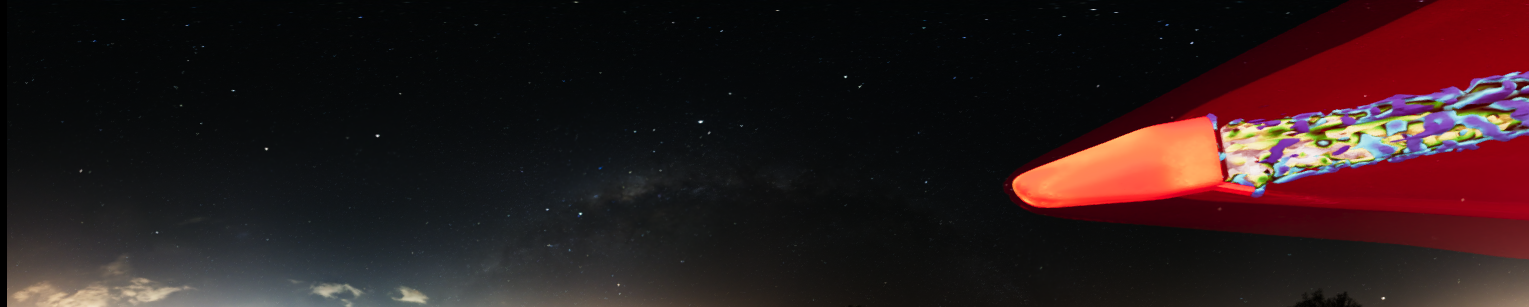
\includegraphics[width=1\linewidth]{chapter1_introduction/pictures/picture_chapter.png}
 \vspace{-2ex}
 \caption{IXV spatial navette by esa}
  \vspace{2ex}
 \label{chap1}
\end{figure}
\minitoc
\thispagestyle{empty}
\newpage
\section {Introduction}

\section{Equations de dynamique des fluides}

Comprendre le comportement des océans, de l'atmosphère et l'écoulement de l'air autour d'un avion ou d'une voiture nécessite de résoudre les équations de Navier-Stokes.

Les équations de Navier-Stokes sont des équations aux dérivées partielles non linéaires qui sont très largement utilisées en hydrodynamique. Elles tirent leur nom de leurs découvreurs au XIXe siècle, le mathématicien et ingénieur français Henri Navier et le physicien et mathématicien britannique George Stokes

Elles décrivent l'évolution dans le temps et dans l'espace du champ de vecteur vitesse des fluides « newtoniens » considérés comme continus. Les ingénieurs les utilisent en aérodynamique pour modéliser le comportement des voitures, des avions à grande vitesse, des navete spatial.


\subsection {Navier-Stokes}
Les équations de Navier-Stokes se formulent à l’aide de bilan de flux de masse, de bilan de flux de quantité de mouvement et de bilan de flux d’énergie du fluide. Pour déterminer l’état d’un milieu fluide, il est nécessaire de connaître en chaque point du domaine : la masse volumique (en kg.m−3), les composantes de la vitesse notées Ui (en m.s−1), la pression P (en Pa), le tenseur des contraintes ij (en N.m−2), les composantes des forces volumiques Fi (en N), la température T (en K), le vecteur densité de flux de chaleur q (en J.m−2.s−1) et l’énergie interne e (en J.kg−1).
En coordonnées cartésiennes, pour une géométrie tridimensionnelle les equations pour un gaz parfait s'écrivent:



\begin{equation}
    \mathbf{U}_t + \mathbf{F}_x + \mathbf{G}_y + \mathbf{H}_z = \mathbf{E}_x^{v,x} + \mathbf{E}_y^{v,y} + \mathbf{E}_z^{v,z} + \mathbf{S},
    \label{eq:cons_ns}
\end{equation}

where the subscripts indicate differentiation, $\mathbf{U}$ is the vector of conservative dimensionless variables and $\mathbf{F}$ ($\mathbf{E}^{v,x}$), $\mathbf{G}$ ($\mathbf{E}^{v,y}$) and $\mathbf{H}$ ($\mathbf{E}^{v,z}$) represent the convective or inviscid (diffusive or viscous) fluxes in $x-$, $y-$ and $z-$direction respectively and $\mathbf{S}$ represents a volumic source term.
Those vectors are defined as such:\\

{\normalsize
\begin{equation}
    \begin{array}{l}
        \mathbf{U} = \left[\begin{array}{c}\rho \\ \rho u \\ \rho v \\ \rho w \\ \rho E\end{array}\right], ~~
        \mathbf{F} = \left[\begin{array}{c}\rho u \\ \rho u^2 + p \\ \rho u v \\ \rho u w \\ \rho u E + p u\end{array}\right], ~~
        \mathbf{G} = \left[\begin{array}{c}\rho v \\ \rho v u \\ \rho v^2 + p \\ \rho v w \\ \rho v E + p v\end{array}\right], ~~
        \mathbf{H} = \left[\begin{array}{c}\rho w \\ \rho w u \\ \rho w v \\ \rho w^2 + p \\ \rho w E + p w\end{array}\right], \\[4em]
        \mathbf{E}^{v,x} = \left[\begin{array}{c}0 \\ \tau_{xx} \\ \tau_{yx} \\ \tau_{zx} \\ \tau_{xx} u + \tau_{xy} v +\tau_{xz} w - q_x\end{array}\right], ~~
        \mathbf{E}^{v,y} = \left[\begin{array}{c}0 \\ \tau_{xy} \\ \tau_{yy} \\ \tau_{zy} \\ \tau_{xy} u + \tau_{yy} v + \tau_{yz} w - q_y\end{array}\right], \\[4em]
        \mathbf{E}^{v,z} = \left[\begin{array}{c}0 \\ \tau_{xz} \\ \tau_{yz} \\ \tau_{zz} \\ \tau_{zx} u + \tau_{zy} v + \tau_{zz} w - q_z\end{array}\right].
    \end{array}
    \label{eq:cons_ns_vectors}
\end{equation}
}\\

In the above dimensionless expressions, $t$ denotes the time and $x$, $y$ and $z$ are the Cartesian coordinates.
$\rho$ denotes density, $u$, $v$ and $w$ denote the $x-$, $y-$ and $z-$direction velocity components respectively, $E$ denotes the specific total energy and $p$ denotes the static pressure.
With the simple perfect gas is considered and therefore the specific total energy can be related to the other variables using:

\begin{equation}
    E = \dfrac{1}{\gamma - 1} \dfrac{p}{\rho} + \dfrac{1}{2}\left( u^2 + v^2 \right),
    \label{eq:perfect_gas_energy}
\end{equation}

where $\gamma$ is the ratio of specific heats and for the perfect gaz hypothesis $\gamma = 1.4$ in the rest of this thesis.

$\mathbf{\tau}$ is the viscous stress tensor.

\begin{equation}
    \tau_{i,j} = 2\mu S_{i,j}
    \label{eq:stres_tensor}
\end{equation}

$S_{i,j}$ deformations tensor defined by:

\begin{equation}
    S_{i,j} = \frac{1}{2}\left(\frac{\partial u_i}{\partial x_j} + \frac{\partial u_j}{\partial x_i} - \frac{2}{3} \frac{\partial u_k}{\partial x_k}\delta_{i,j}\right)
    \label{eq:stres_tensor_deformation}
\end{equation}
and $\mathbf{q}$ the heat flux vector.

$\mu$ is the dynamic viscosity compute with the Sutherland law.

\begin{equation}
    \mu(T) = \mu_{ref}\left(\frac{T}{T_{ref}}\right)^{3/2} + \frac{T_{ref}+S}{T+S}, \quad with \quad S = 110.4 K.
    \label{eq:mu_sutherland}
\end{equation}

\begin{equation}
    q = -\lambda\nabla T
    \label{eq:stres_tensor}
\end{equation}

With $\nabla T$ are the gradient of temperature, $\lambda = C_p\mu/P_r$ the thermic conductivity, $C_p$ specific gaz constant and $P_r$ the Prandl number with $P_r = 0.72 $for laminar flow and $P_r = 0.9$ for turbulent flow.

\subsection{Simulation RANS}

L'approche RANS utilisent un opérateur de moyenne statistique(add ref ). Les equation obtenue à l'aide des opérateurs est un systeme d'équation ouvert. Plusieurs modéle de turbulence permettent de fermé le systeme d'equation RANS. Les plus connus sont les modéles k-omega sst de Mender[ref], le modele spalart allmaras de P.R. Spalart (ref)et le modele k epesilon de Jones, W. P., and Launder, B. E. (1972).\\
Les calculs RANS reposent sur des equatons moyenné et génerent donc des champs d'écoulement moyen. Cette Methode est le plus souvent utilisé pour des calculs stationnaires. Ils sont tres utilisé dans le monde de l'industrie des calculs turbulent pour sont cout de calculs qui est tres interresant.\\
Cependant en moyennant les variables turbulente il est imossible de calculer les fluctuations de ces varaibles au cours du temps à contrario des autres methodes. Comme représenté sur la figure (ref fig) lors de dimensionnment d'enjin spaciaux il est crucial d'obtenir des fluctuations au cours du temps, pour la pression ou la temperature. Si lors d'une rentré atmopherique, les materiuax d'une vehicule atteignent une température de fusion, le matériaux sera dégradé et cela pourra enjendrer des consequances terribles lors d' une mission.

\begin{figure}[h!]
 \centering
 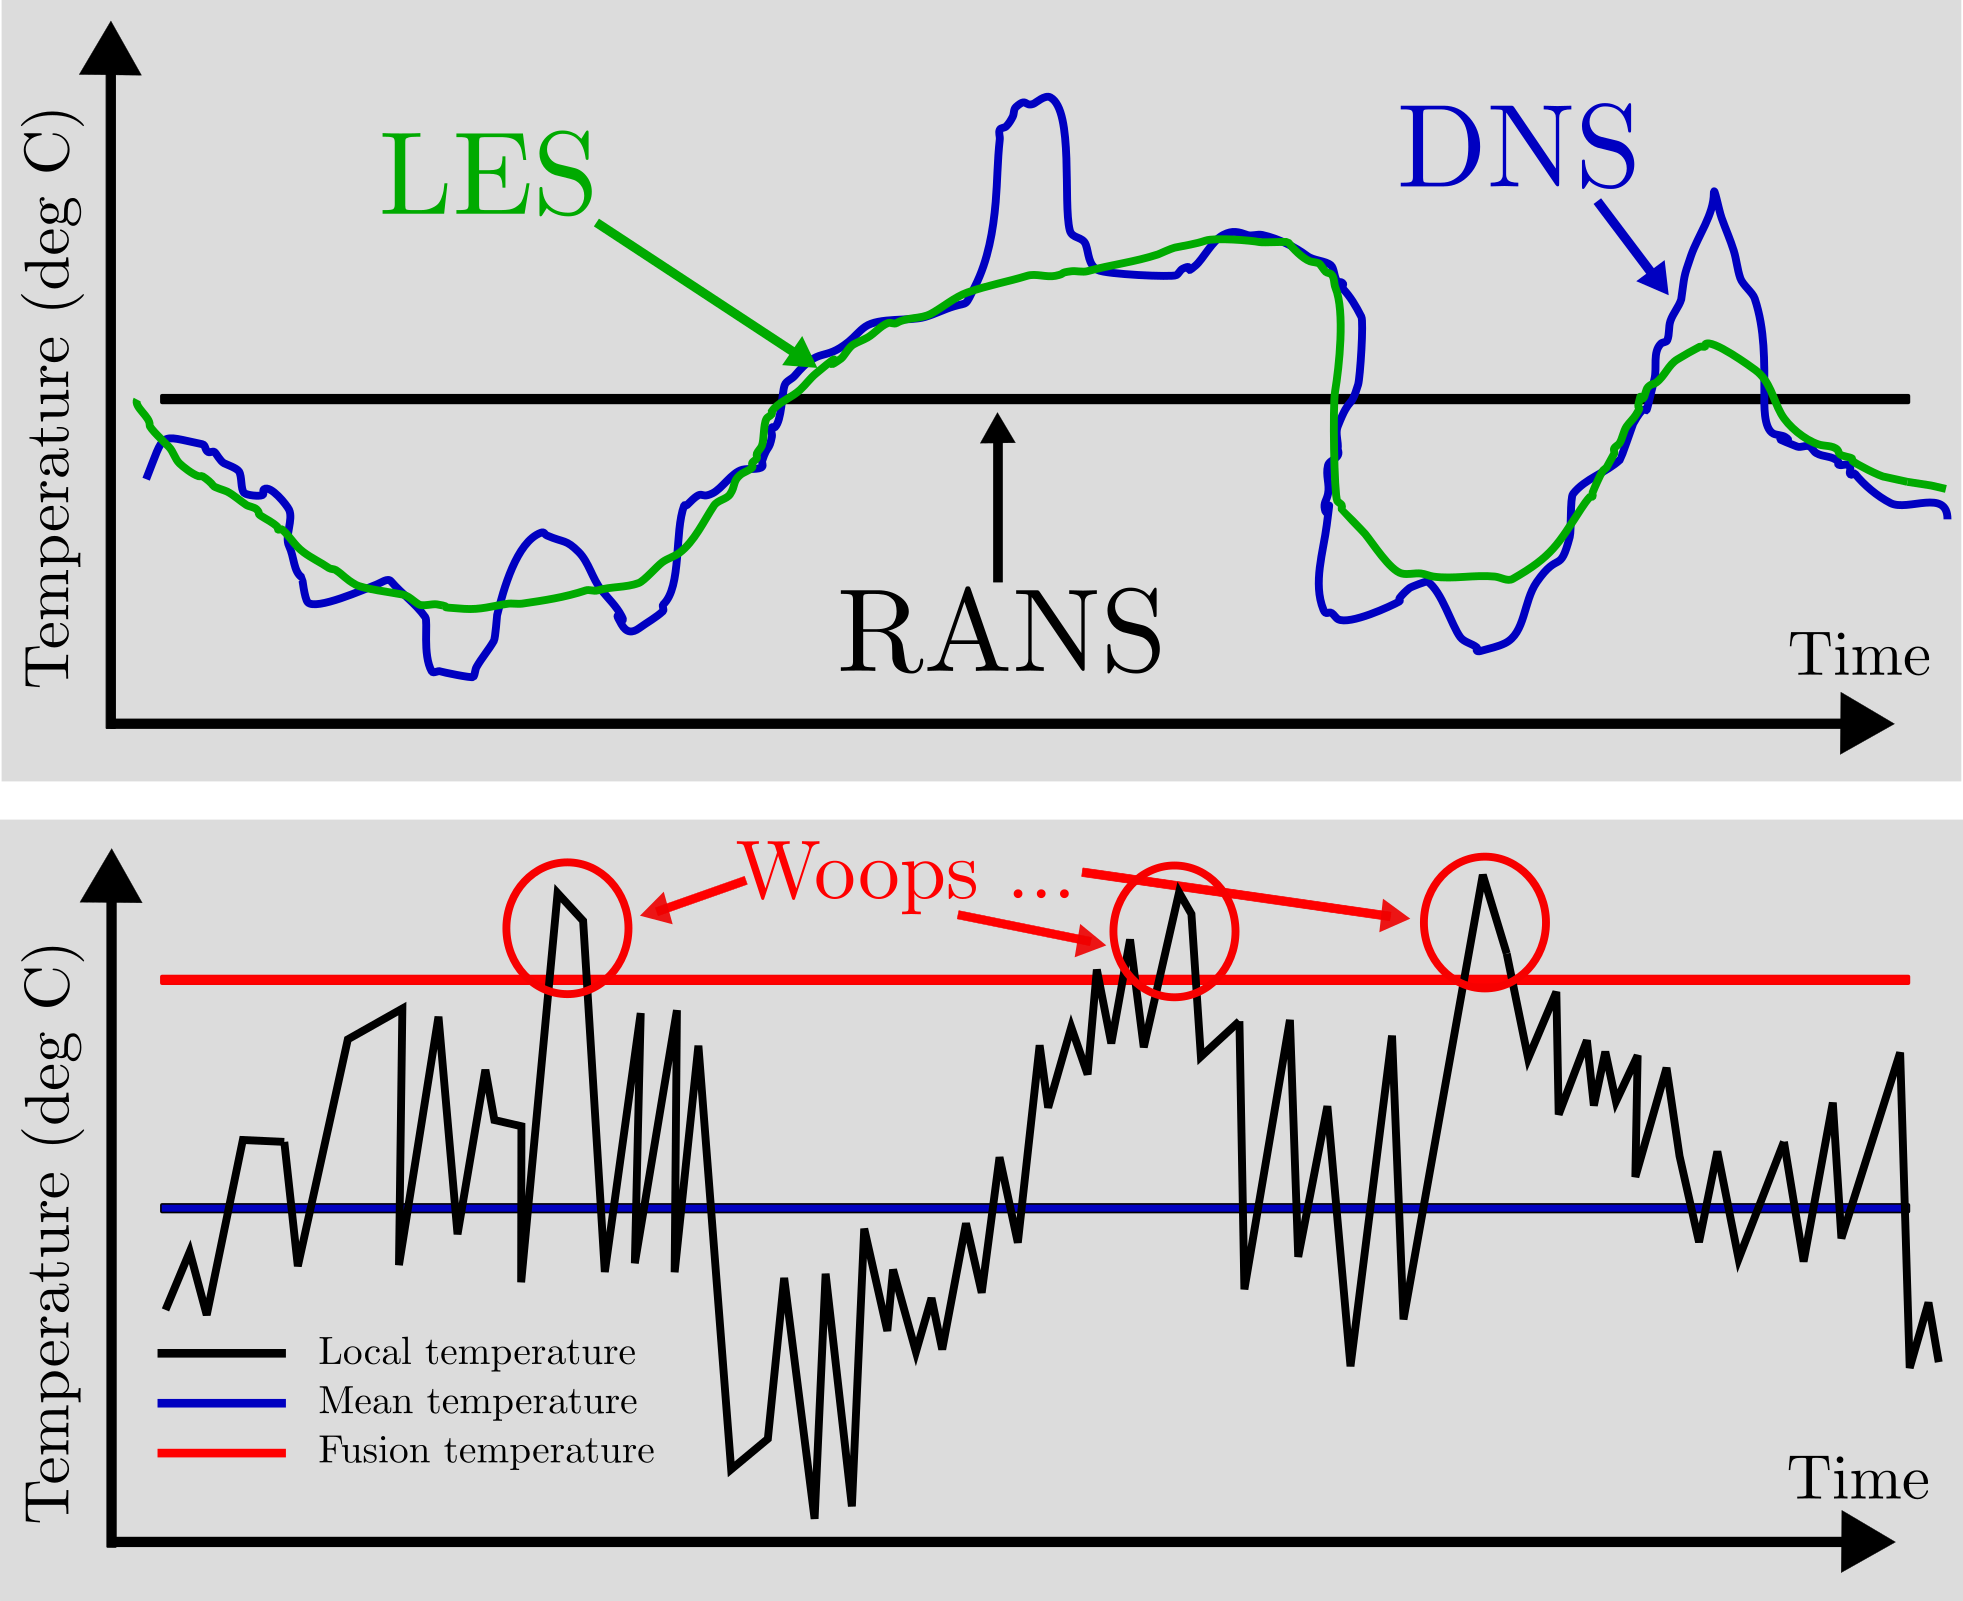
\includegraphics[width=0.7\linewidth]{chapter1_introduction/pictures/les_rans_dns.png}
 \vspace{-2ex}
 \caption{IXV spatial navette by esa}
  \vspace{2ex}
 \label{rans}
\end{figure}

\section {DNS\_LES\_RANS}


\subsection{Simulation des Grandes Échelles}

Une alternative aux deux approches précédentes est la simulation des grandes échelles, appelée Large-Eddy Simulation (LES) en anglais. Contrairement à la DNS qui résout toutes les échelles de turbulence, la LES ne représente que les grandes structures turbulentes. L'approche LES repose sur les hypothèses de similitudes de Kolmogorov [78]. Selon ces hypothèses, les grandes structures turbulentes porteuses d'énergie caractérisent l'écoulement et doivent donc être calculées, alors que le comportement des petites structures turbulentes responsables de la dissipation visqueuse peut être modélisé. En pratique, un filtre passe-bas $G$ est appliqué aux équations de Navier-Stokes pour séparer les échelles de l'écoulement qui sont calculées par les équations de celles qui sont modélisées. Les effets dissipatifs des petites échelles qui ne sont pas résolues par la LES sont pris en compte en utilisant un modèle dit "de sous-maille". Ainsi, comme la LES ne calcule pas toutes les échelles de la turbulence, le nombre de points nécessaire dans le maillage est moins important par rapport à une DNS. Pour une turbulence isotrope dans une boîte de volume égal à $L^{3}$, il varie en fonction du nombre de Reynolds comme $R e_{L}^{3 / 2}$ [6]. La LES permet donc de considérer des écoulements à des nombres de Reynolds plus élevés que la DNS, de l'ordre de $R e_{D}=10^{5}$ pour les jets simples flux [16, 25]. En revanche, compte tenu des ressources de calcul disponibles, la LES reste hors d'atteinte pour les écoulements de jets double-flux installés à $R e_{D}=10^{6}$ considérés dans chapitre 1. Simulations du bruit des jets

l'industrie. Les développements numériques réalisés dans cette thèse visent à rendre réalisable la LES pour de tels écoulements.

\begin{figure}[h!]
 \centering
 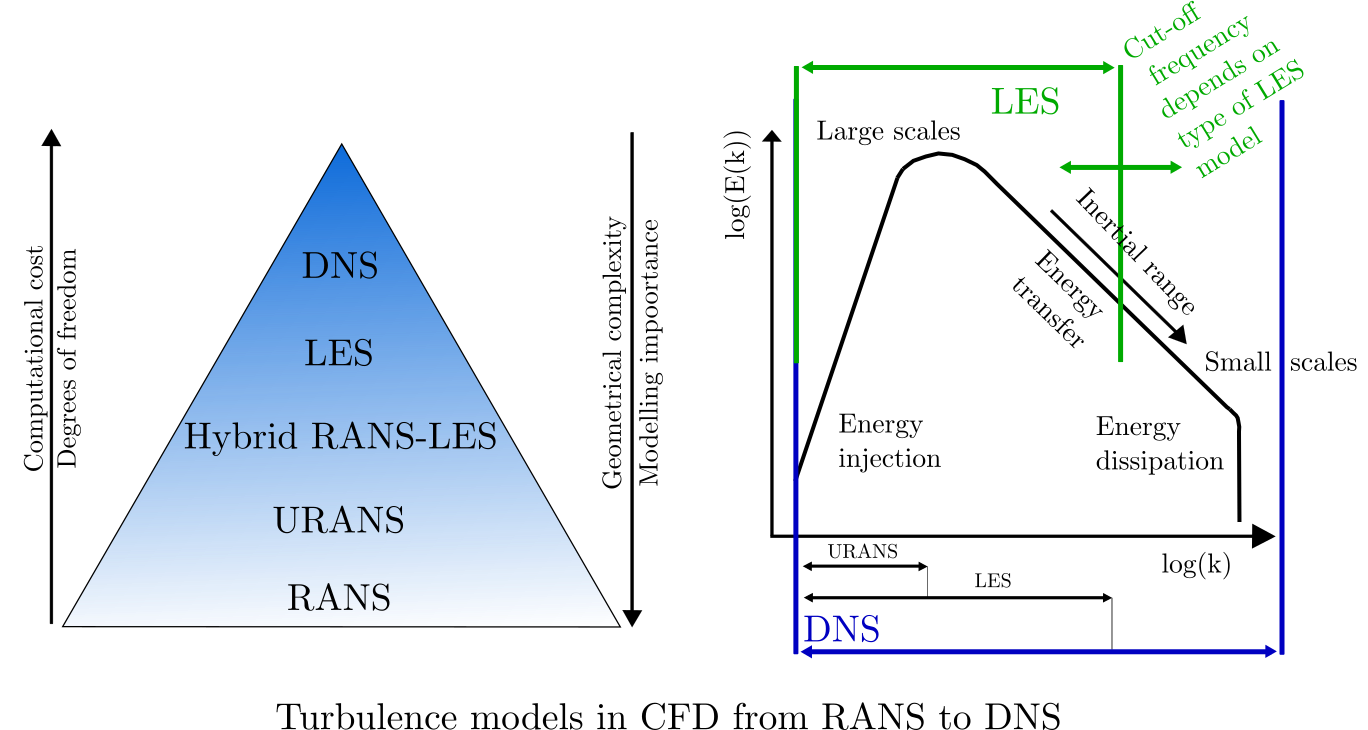
\includegraphics[width=1.0\linewidth]{chapter1_introduction/pictures/les.png}
 \vspace{-2ex}
 \caption{IXV spatial navette by esa}
  \vspace{2ex}
 \label{les}
\end{figure}

\section{Conclusion}

Une alternative aux deux approches précédentes est la simulation des grandes échelles, appelée Large-Eddy Simulation (LES) en anglais. Contrairement à la DNS qui résout toutes les échelles de turbulence, la LES ne représente que les grandes structures turbulentes. L'approche LES repose sur les hypothèses de similitudes de Kolmogorov [78]. Selon ces hypothèses, les grandes structures turbulentes porteuses d'énergie caractérisent l'écoulement et doivent donc être calculées, alors que le comportement des petites structures turbulentes responsables de la dissipation visqueuse peut être modélisé. En pratique, un filtre passe-bas $G$ est appliqué aux équations de Navier-Stokes pour séparer les échelles de l'écoulement qui sont calculées par les équations de celles qui sont modélisées. Les effets dissipatifs des petites échelles qui ne sont pas résolues par la LES sont pris en compte en utilisant un modèle dit "de sous-maille". Ainsi, comme la LES ne calcule pas toutes les échelles de la turbulence, le nombre de points nécessaire dans le maillage est moins important par rapport à une DNS. Pour une turbulence isotrope dans une boîte de volume égal à $L^{3}$, il varie en fonction du nombre de Reynolds comme $R e_{L}^{3 / 2}$ [6]. La LES permet donc de considérer des écoulements à des nombres de Reynolds plus élevés que la DNS, de l'ordre de $R e_{D}=10^{5}$ pour les jets simples flux [16, 25]. En revanche, compte tenu des ressources de calcul disponibles, la LES reste hors d'atteinte pour les écoulements de jets double-flux installés à $R e_{D}=10^{6}$ considérés dans chapitre 1. Simulations du bruit des jets

l'industrie. Les développements numériques réalisés dans cette thèse visent à rendre réalisable la LES pour de tels écoulements.


\chapter{Méthode numérique du code Hyperion en 2D}

\minitoc
\thispagestyle{empty}
\newpage
\subsection{Cartesian fluid domain discretization}\label{ssec:cartesian}

In this particular study, we use only Cartesian grids with constant grid spacings $\Delta x$, $\Delta y$ and $\Delta z$.
Based on such a mesh, the finite-volume method \cite{leveque2002finite} is employed for space discretization of the compressible Navier-Stokes equations~\eqref{eq:cons_ns}.
An exhaustive description of the technique adapted to Cartesian grids is given in~\cite{BRIDELBERTOMEU2021}: we shall only present here a few select details to expose the core of HYPERION.

\subsubsection{Mixed finite-volume/finite-difference numerical scheme}\label{sssec:num_scheme}

In HYPERION, when solving numerically the Navier-Stokes equations~\eqref{eq:cons_ns}, we mix a finite-volume flux-balance formulation for the hyperbolic terms ($\mathbf{F}_x$, $\mathbf{G}_y$ and $\mathbf{H}_z$) and a finite-difference formulation of the gradients involved in the parabolic terms ($\mathbf{E}^{v}_{x,y,z}$) whereas the (optional) source terms are computed directly at the cell centers.
The flux-balance is obtained with numerical fluxes computed at each face of each cell using an approximate Riemann solver \cite{toro2013riemann} relying on left- and right-interpolated values from the neighboring cells.
The mathematical expression of this mix formulation, as well as a selection of reconstructions and Riemann solvers present in HYPERION will be discussed in the following paragraphs.

% Addition here :
% + in a few lines, total discretization in space with intro of interpolations and Riemann solvers that we discuss right after :

Considering that in the present case all cells are quadrangles, the flux-balance can be split by direction, and the final mathematical expression of the space discretization used in HYPERION can be written in cell $c$ as:

\begin{equation}
    \begin{split}
        \dfrac{d\overline{\mathbf{U}}_c}{dt} &= -\dfrac{\hat{\mathbf{F}}_{i+1/2,j,k} - \hat{\mathbf{F}}_{i-1/2,j,k}}{\Delta x}
        - \dfrac{\hat{\mathbf{G}}_{i,j+1/2,k} - \hat{\mathbf{G}}_{i,j-1/2,k}}{\Delta y}
        - \dfrac{\hat{\mathbf{H}}_{i,j,k+1/2} - \hat{\mathbf{H}}_{i,j,k-1/2}}{\Delta z}
        \\
        &+ \mathcal{D}_x\left( \mathbf{E}^{v,x}_{c} \right)
         + \mathcal{D}_y\left( \mathbf{E}^{v,y}_{c} \right)
         + \mathcal{D}_z\left( \mathbf{E}^{v,z}_{c} \right)
         + \mathbf{S}_c
    \end{split}
    \label{eq:fvm_discretization}
\end{equation}

where $i$, $j$ and $k$ are the indices of cell $c$ along each direction, and $i\pm1/2$, $j\pm1/2$ and $k\pm1/2$ represent the faces of the cell in each direction as well.

The vector $\hat{\mathbf{F}}$ (resp. $\hat{\mathbf{G}}$, $\hat{\mathbf{H}}$) is a numerical approximation of the inviscid physical flux $\mathbf{F}$ (resp. $\mathbf{G}$, $\mathbf{H}$) at the faces of the cell of interest and can be expressed in a most general manner as:

\begin{equation}
    \hat{\mathbf{F}}_{i\pm1/2,j,k} = \mathcal{U}\left( \mathbf{F}^{L}_{i\pm1/2,j,k}, \mathbf{F}^{R}_{i\pm1/2,j,k},
    \overline{\mathbf{U}}^{L}_{i\pm1/2,j,k}, \overline{\mathbf{U}}^{R}_{i\pm1/2,j,k} \right),
    \label{eq:num_approx_flux}
\end{equation}

where $\mathcal{U}$ stands for a generic approximate Riemann solver while the superscripts $L$ and $R$ designate respectively the left- and right-biased reconstruction of either $\mathbf{F}$ or $\overline{\mathbf{U}}$ at the faces of the cell of interest.
A similar expression stands for $\hat{\mathbf{G}}_{i, j \pm 1/2,k}$ and $\hat{\mathbf{H}}_{i, j,k \pm 1/2}$.

The derivatives involved in $\boldsymbol{\tau}$ and $\mathbf{q}$ are computed as follows for any variable $\varphi$ in cell $(i,j,k)$ and along any dimension $d\in\lbrace x,y,z \rbrace$:

\begin{equation}
    \dfrac{\partial \varphi_{i,j,k}}{\partial d} = \mathcal{D}_d\left( \varphi_{i,j,k} \right),
\end{equation}

where $\mathcal{D}_d$ represents a centered finite-difference-like differentiation operator along dimension $d$.
In this study we use either a second- or a fourth-order operator, respectively denoted $\mathcal{D}^{(2)}_d$ and $\mathcal{D}^{(4)}_d$.
They are defined as:

\begin{equation}
    \mathcal{D}^{(2)}_d(\varphi_{i,j,k}) = \dfrac{\varphi_{i+1,j,k} - \varphi_{i-1,j,k}}{2\Delta d},
    \label{eq:para_operator_2}
\end{equation}

and

\begin{equation}
    \mathcal{D}^{(4)}_d(\varphi_{i,j,k}) = \dfrac{\varphi_{i-2,j,k} - 8\varphi_{i-1,j,k} + 8\varphi_{i+1,j,k} - \varphi_{i+2,j,k}}{12\Delta d}.
    \label{eq:para_operator_4}
\end{equation}

\subsubsection{Reconstruction schemes}\label{sssec:interpolations}

As mentioned in introduction to section~\ref{sec:short_hyperion}, HYPERION is designed to provide numerical predictions of viscous compressible flows.
In particular, we are interested in hypersonic regimes where the Mach number and the Reynolds number are very high.
In layman terms, the flow will therefore exhibit very strong large scale discontinuities (shock \& contact waves) as well as small scale viscous eddies - HYPERION has to capture both.
To do so, we turned to high-order reconstructions (to capture the smallest scales) with good properties in the presence of discontinuities, especially that have a non-oscillatory property preventing too strong over- and under-shoots in the vicinity of discontinuities.

The well-known family of WENO-Z schemes\footnote{WENO stands for Weighted Essentially Non-Oscillatory.} was added to HYPERION \cite{liu1994weighted,jiang1996efficient,hu2010adaptive,henrick2005mapped} for their robustness and their theoretical high-order.
Satisfactory results were obtained in the hypersonic regime, although the viscous small scales tended to be too dissipated.

This last comment pushed us to implement and use the newer generation of TENO \cite{fu2016family,hu2011scale} schemes\footnote{TENO stands for Targeted Essentially Non-Oscillatory.} that allow for better discrimination between the large discontinuous events and the small eddies produced by viscous turbulence.
The interested reader is referred to the family of papers by Fu \emph{et al.} for more details \cite{fu2016family,fu2017targeted,fu2018new,fu2019low,fu2019very}, while we only recall below the $5^{\text{th}}$-order formulation that we make most use of.

\begin{equation}
    \overline{\mathbf{U}}^L_{i+1/2,j,k} =
    \begin{aligned}
          & \; \omega_1\; \times \left[ \overline{\mathbf{U}}_{i+1/2,j,k}^{L,1} = \dfrac{1}{6} \left({-\overline{\mathbf{U}}}_{i-1,j,k} + 5{\overline{\mathbf{U}}}_{i,j,k} + 2{\overline{\mathbf{U}}}_{i+1,j,k} \right) \right]\\
        + & \; \omega_2\; \times \left[ \overline{\mathbf{U}}_{i+1/2,j,k}^{L,2} = \dfrac{1}{6} \left({2\overline{\mathbf{U}}}_{i,j,k} + 5 {\overline{\mathbf{U}}}_{i+1,j,k} - {\overline{\mathbf{U}}}_{i+2,j,k} \right) \right]\\
        + & \; \omega_3\; \times \left[ \overline{\mathbf{U}}_{i+1/2,j,k}^{L,3} = \dfrac{1}{6} \left({2\overline{\mathbf{U}}}_{i-2,j,k} - 7{\overline{\mathbf{U}}}_{i-1,j,k} + 11{\overline{\mathbf{U}}}_{i,j,k} \right) \right]\\
    \end{aligned}
    \label{eq:teno5}
\end{equation}

where $\omega_{1,2,3}$ are nonlinear weights.
To define $\omega_k$ we need to calculate the $\gamma_k$, \emph{a.k.a.} the smoothness indicators:

\begin{equation}
  \gamma_k = \left(C + \dfrac{\tau_k}{\beta_k +\epsilon}\right)^q
  \label{eq:teno5_smooth}
\end{equation}

where $C$ is set to $1$, $q$ is hardcoded to $6$, and $\epsilon$ is an input parameter typically kept very small ; in this study we use $10^{-6}$.
The per-stencil finite-difference operators $\beta_k$ are given by:

\begin{equation}
    \begin{aligned}
        \beta_1 &=&  \dfrac{1}{4}({\bf f}_{j-1} - {\bf f}_{j+1})^2 + \dfrac{13}{12}({\bf f}_{j-1} - 2{\bf f}_{j}+{\bf f}_{j+1})^2 \\[0.5em]
        \beta_2 &=&  \dfrac{1}{4}({3\bf f}_{j} - {4\bf f}_{j+1} + {\bf f}_{j+2})^2 + \dfrac{13}{12}({\bf f}_{j} - 2{\bf f}_{j+1}+{\bf f}_{j+2})^2 \\[0.5em]
        \beta_3 &=&  \dfrac{1}{4}({\bf f}_{j-2} - {4\bf f}_{j-1} + {3\bf f}_{j})^2 + \dfrac{13}{12}({\bf f}_{j-2} - 2{\bf f}_{j-1}+{\bf f}_{j})^2 \\
    \end{aligned}
    \label{eq:teno5_betas}
\end{equation}

and

\begin{equation}
    \tau_k = \left\vert\beta_k - \dfrac{1}{6}(\beta_2 + \beta_3 + 4\beta_1)\right\vert,\; k=1,2,3.
    \label{eq:teno5_tau}
\end{equation}

Now we need to also define the scale-separator parameter $\chi_k$ (on which we rely most to discriminate between the large-scale discontinuities and the small-scale eddies) and the sharp cut-off function $\delta_k$ (on which we rely to handle large-scale discontinuities):

\begin{equation}
  \chi_k = \dfrac {\gamma_k} {\sum_{j=1}^3 \gamma_j }, k = 1,2,3
  \label{eq:teno5_chi}
\end{equation}

\begin{equation}
  \delta_k =  0 \quad \text{if} \quad \chi_k < C_T \quad \text{otherwise} \quad \delta_k=1,\; k = 1,2,3,
  \label{eq:teno5_delta}
\end{equation}

where $C_T$ is a very small value - here, $10^{-5}$.
With all this, the nonlinear weights $\omega_k$ can be defined as:

\begin{equation}
  \omega_k = \dfrac {a_k} {\sum_{j=1}^3 a_j },\; k = 1,2,3
\end{equation}

where

\begin{equation}
    a_1 = \dfrac{6}{10}\delta_1,\quad
    a_2 = \dfrac{3}{10}\delta_2,\quad
    a_3 = \dfrac{1}{10}\delta_3.\quad
\end{equation}

Note that to deal with the large stencil close to the edges of the Cartesian domain, HYPERION uses ghost cells - an illustration in two dimensions is provided on figure~\ref{fig:ghost_cells}.

\begin{figure}[ht!]
    \centering
    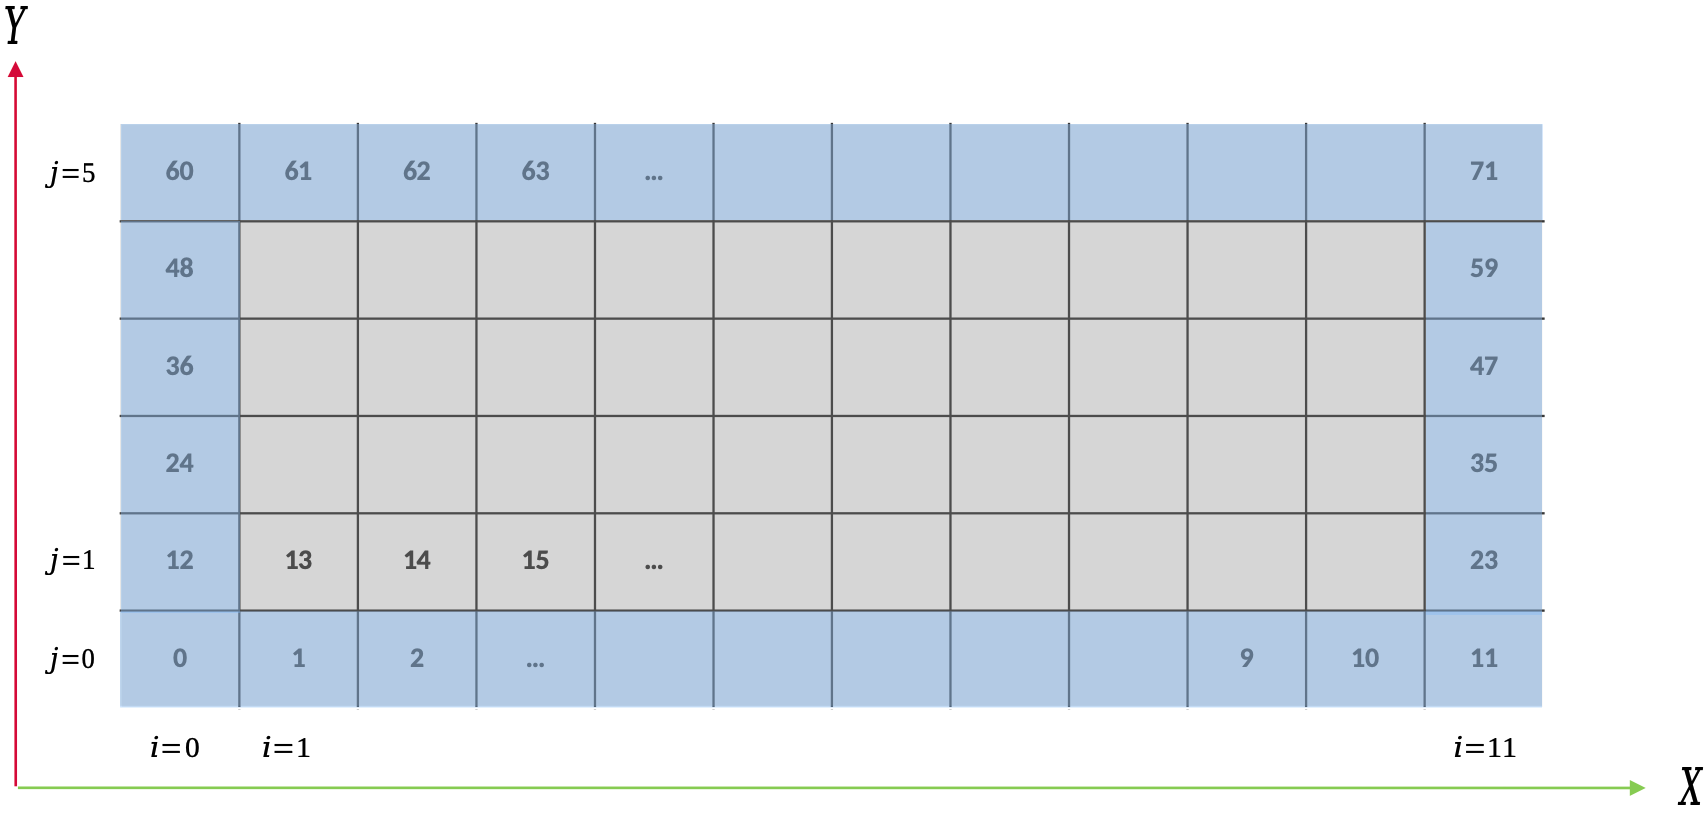
\includegraphics[width=0.75\linewidth]{chapter3_numerical_methods/pictures/grid_ghost_2.png}
    \caption{
        Illustration of the ghost cells layer (blue cells) around the Cartesian grid in HYPERION.
        The numbering of the cells is also shown.
        Note that the three-dimensional Cartesian meshes are handled in the same fashion, with index $i$ in the $X$ direction evolving the fastest, followed by $j$ in the $Y$ direction, then $k$ in the $Z$ direction.
    }
    \label{fig:ghost_cells}
\end{figure}

\subsubsection{Approximate Riemann solvers}\label{sssec:ars}

Once the fields have been reconstructed at each face of each cell (see paragraph~\ref{sssec:interpolations} above), the left/right discontinuous problem (see equation~\eqref{eq:num_approx_flux}) is solved approximately using a Riemann solver.
The most used approximate solvers can be grouped in three large families: Flux Difference Splitting (FDS), Flux Vector Splitting (FVS) and Flux Type Splitting (FTS) \cite{toro2013riemann,qu2021review}.
In HYPERION we focus on two types of solvers in particular, FDS solvers that work as a finite volume method to solve the Riemann problem and FVS Riemann solvers that combine the qualities of the other two families by separating kinematic and acoustic scales.

Several approximate Riemann solvers have therefore been implemented in HYPERION to serve different purpose.
In the present study, similarly to the need for a reconstruction able to handle large and small scales simultaneously, the Riemann solver we were seeking had to have the ability to behave well in both high and low-Mach regimes (see \emph{e.g.} \cite{maier2021su2}) and to not trigger the well-known carbuncle instability\cite{kitamura2012carbuncle}.
% especially in the cases where "dead water" recirculation regions could appear in the flow because of the obstacles.
A series of tests and a bibliographic study lead us to opt in for a FVS solver constructed by Liou \emph{et al.}, the AUSM$^+$-up \cite{liou1996sequel,liou2006sequel} because of its robustness and its increased level of accuracy at all speeds.
Presenting the details of the mathematical implementations is out of the scope of this paper but the interested reader is referred to the aforementioned papers.

\subsection{Sharp immersed boundary conditions}\label{ssec:ibc}

\begin{figure}[ht!]
    \centering
    \begin{tabular}{ccc}
        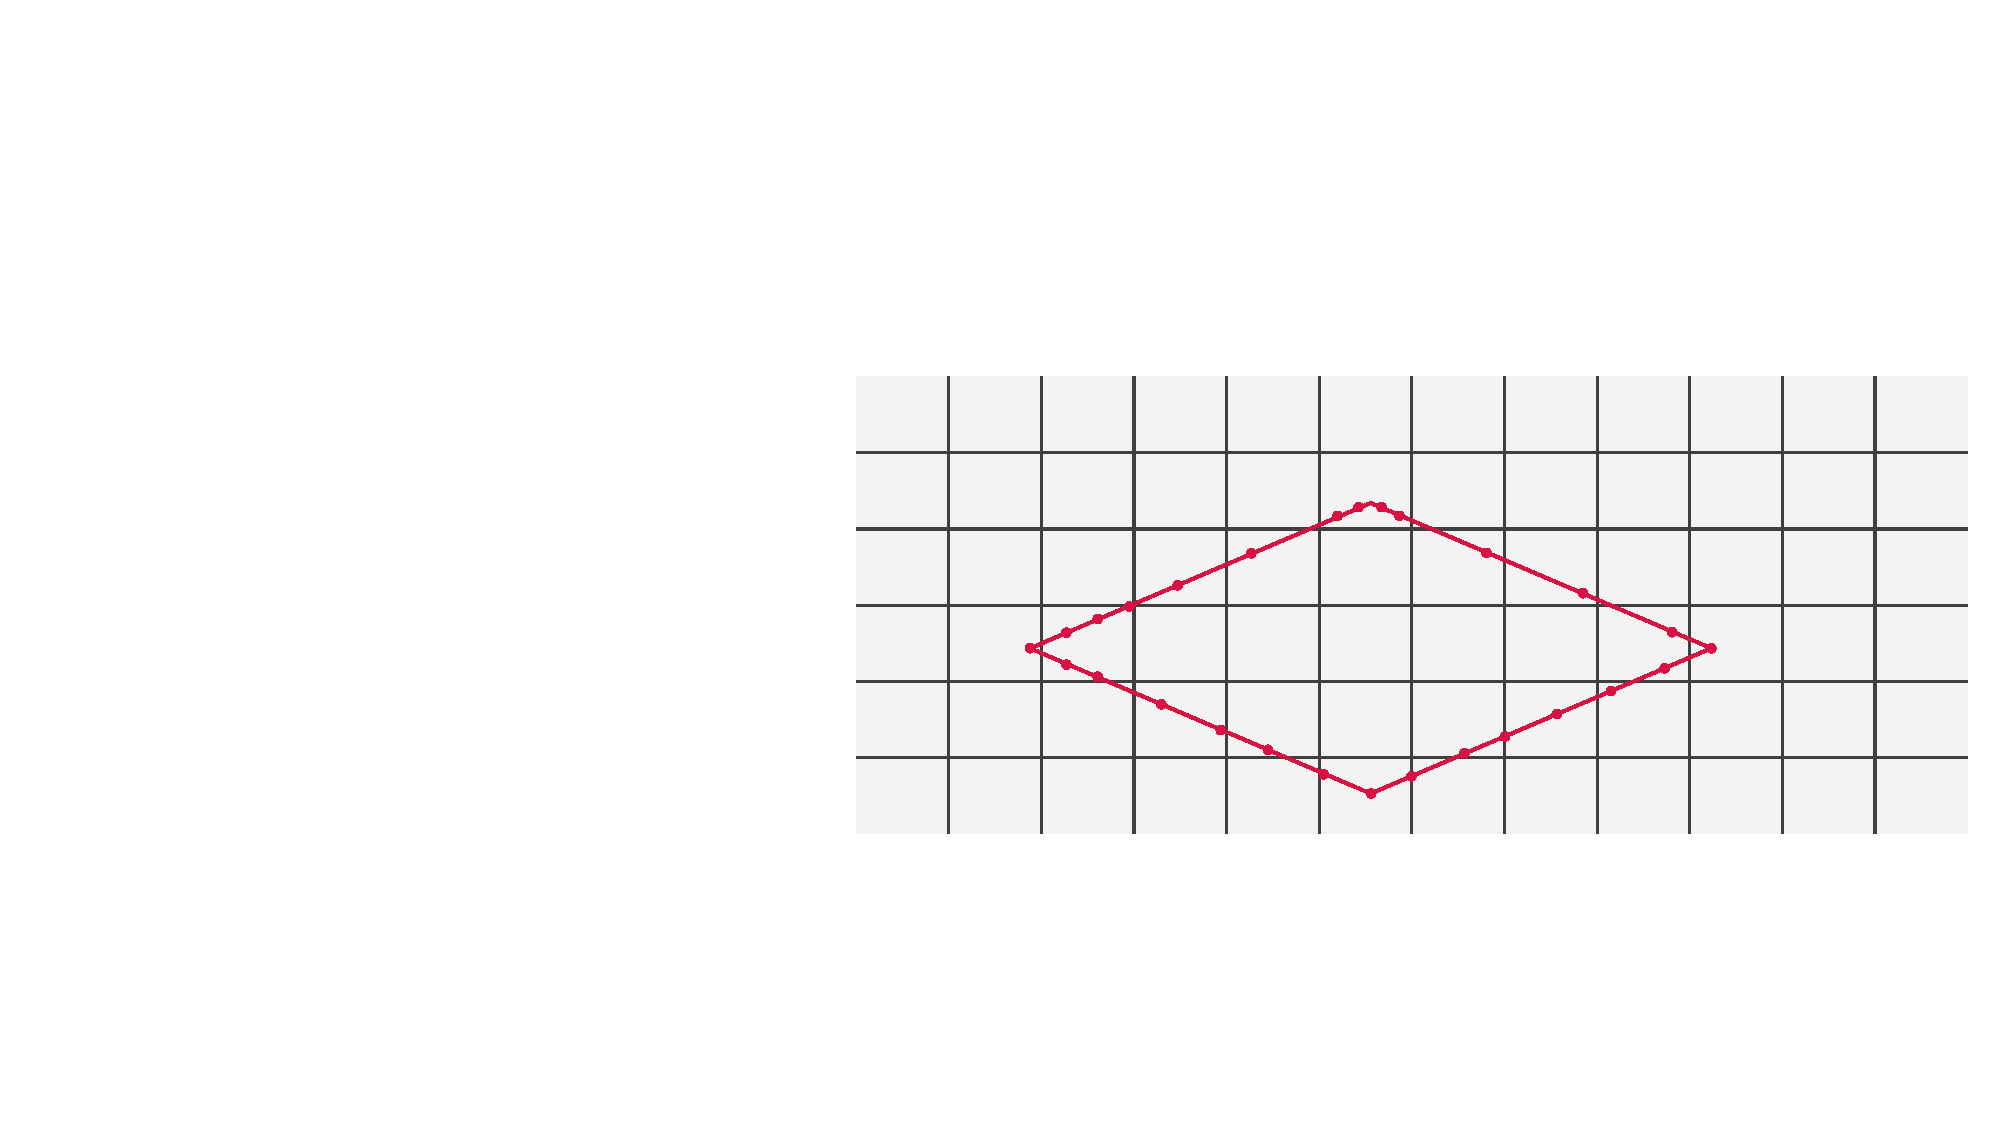
\includegraphics[width=0.3\linewidth]{chapter3_numerical_methods/pictures/ibm1.pdf} &
        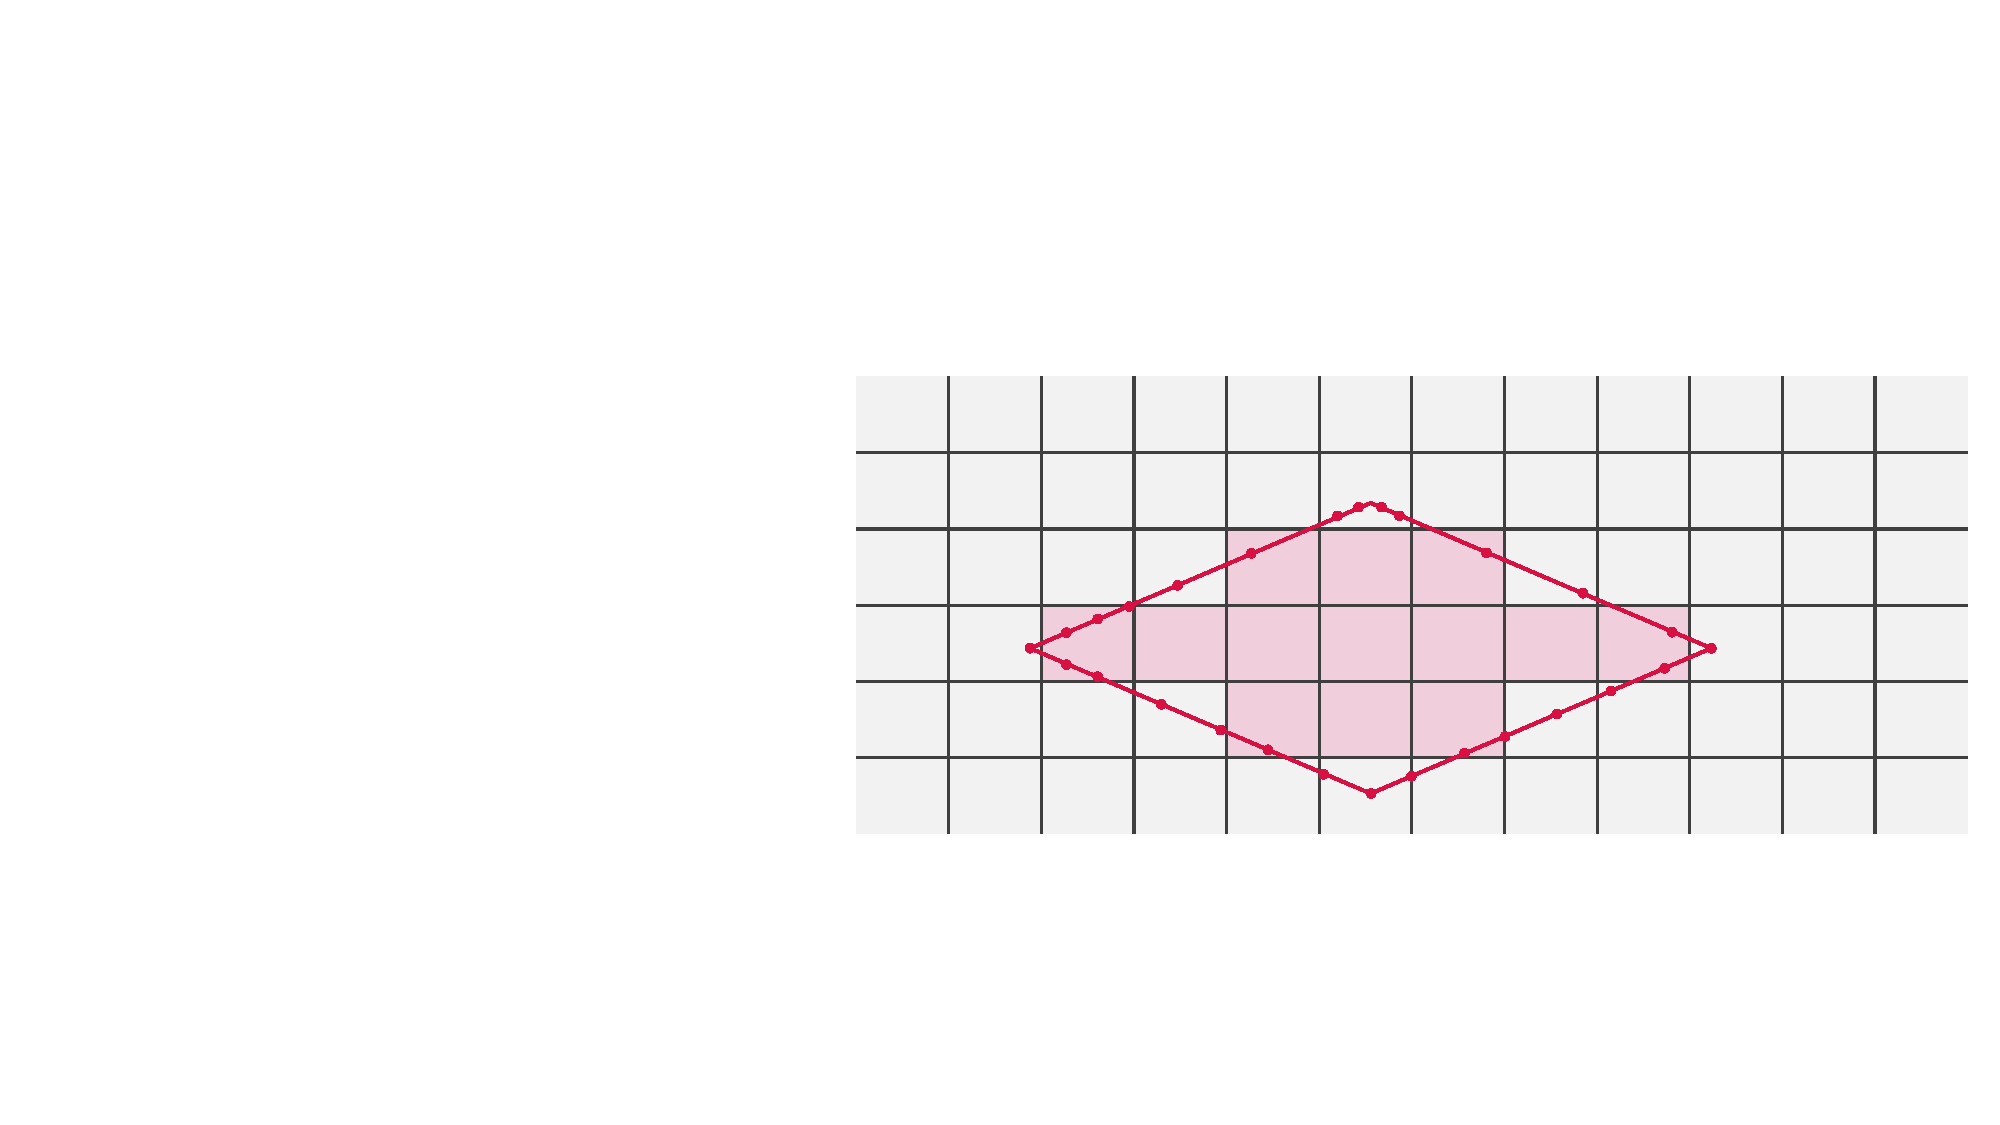
\includegraphics[width=0.3\linewidth]{chapter3_numerical_methods/pictures/ibm2.pdf} &
        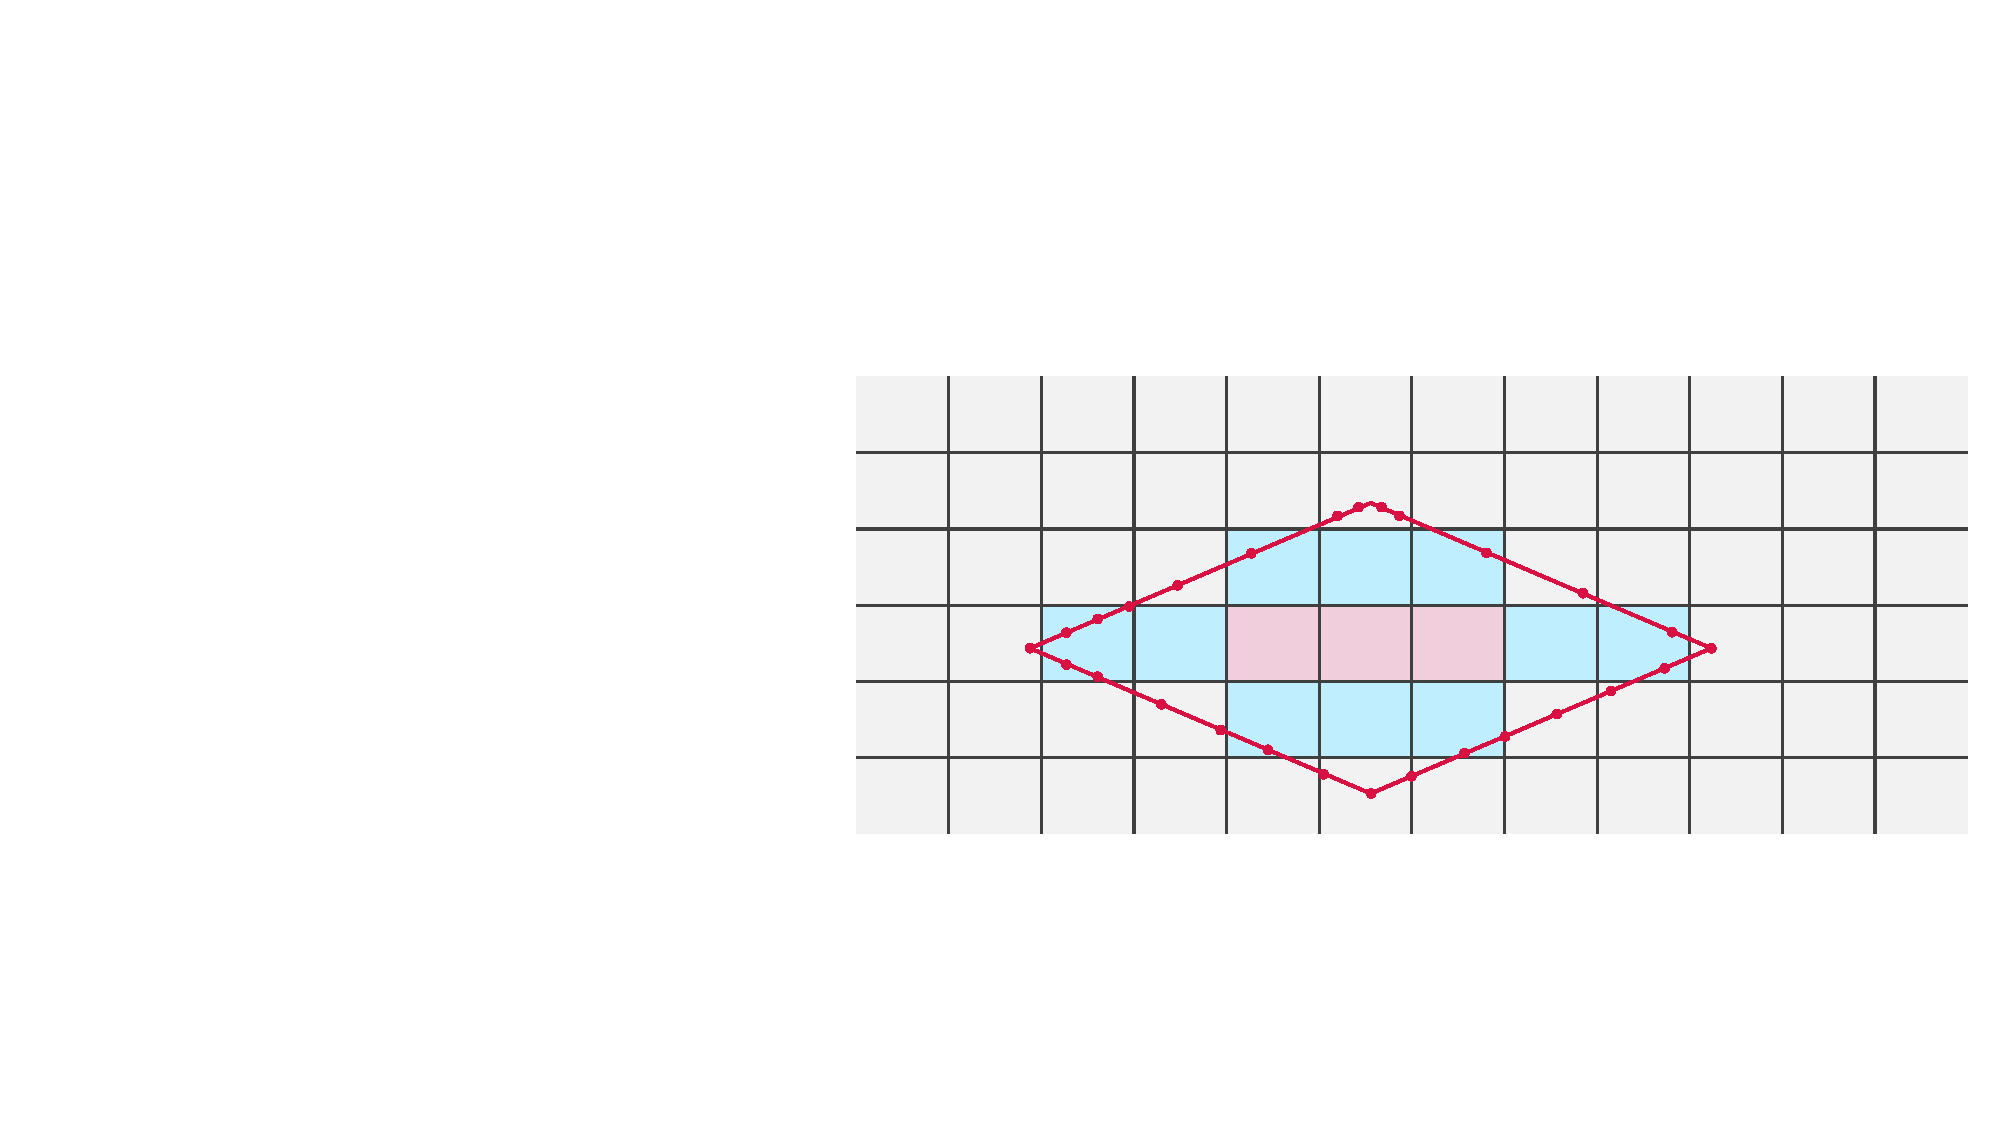
\includegraphics[width=0.3\linewidth]{chapter3_numerical_methods/pictures/ibm3.pdf} \\[0.4em]
        (a) & (b) & (c) \\
        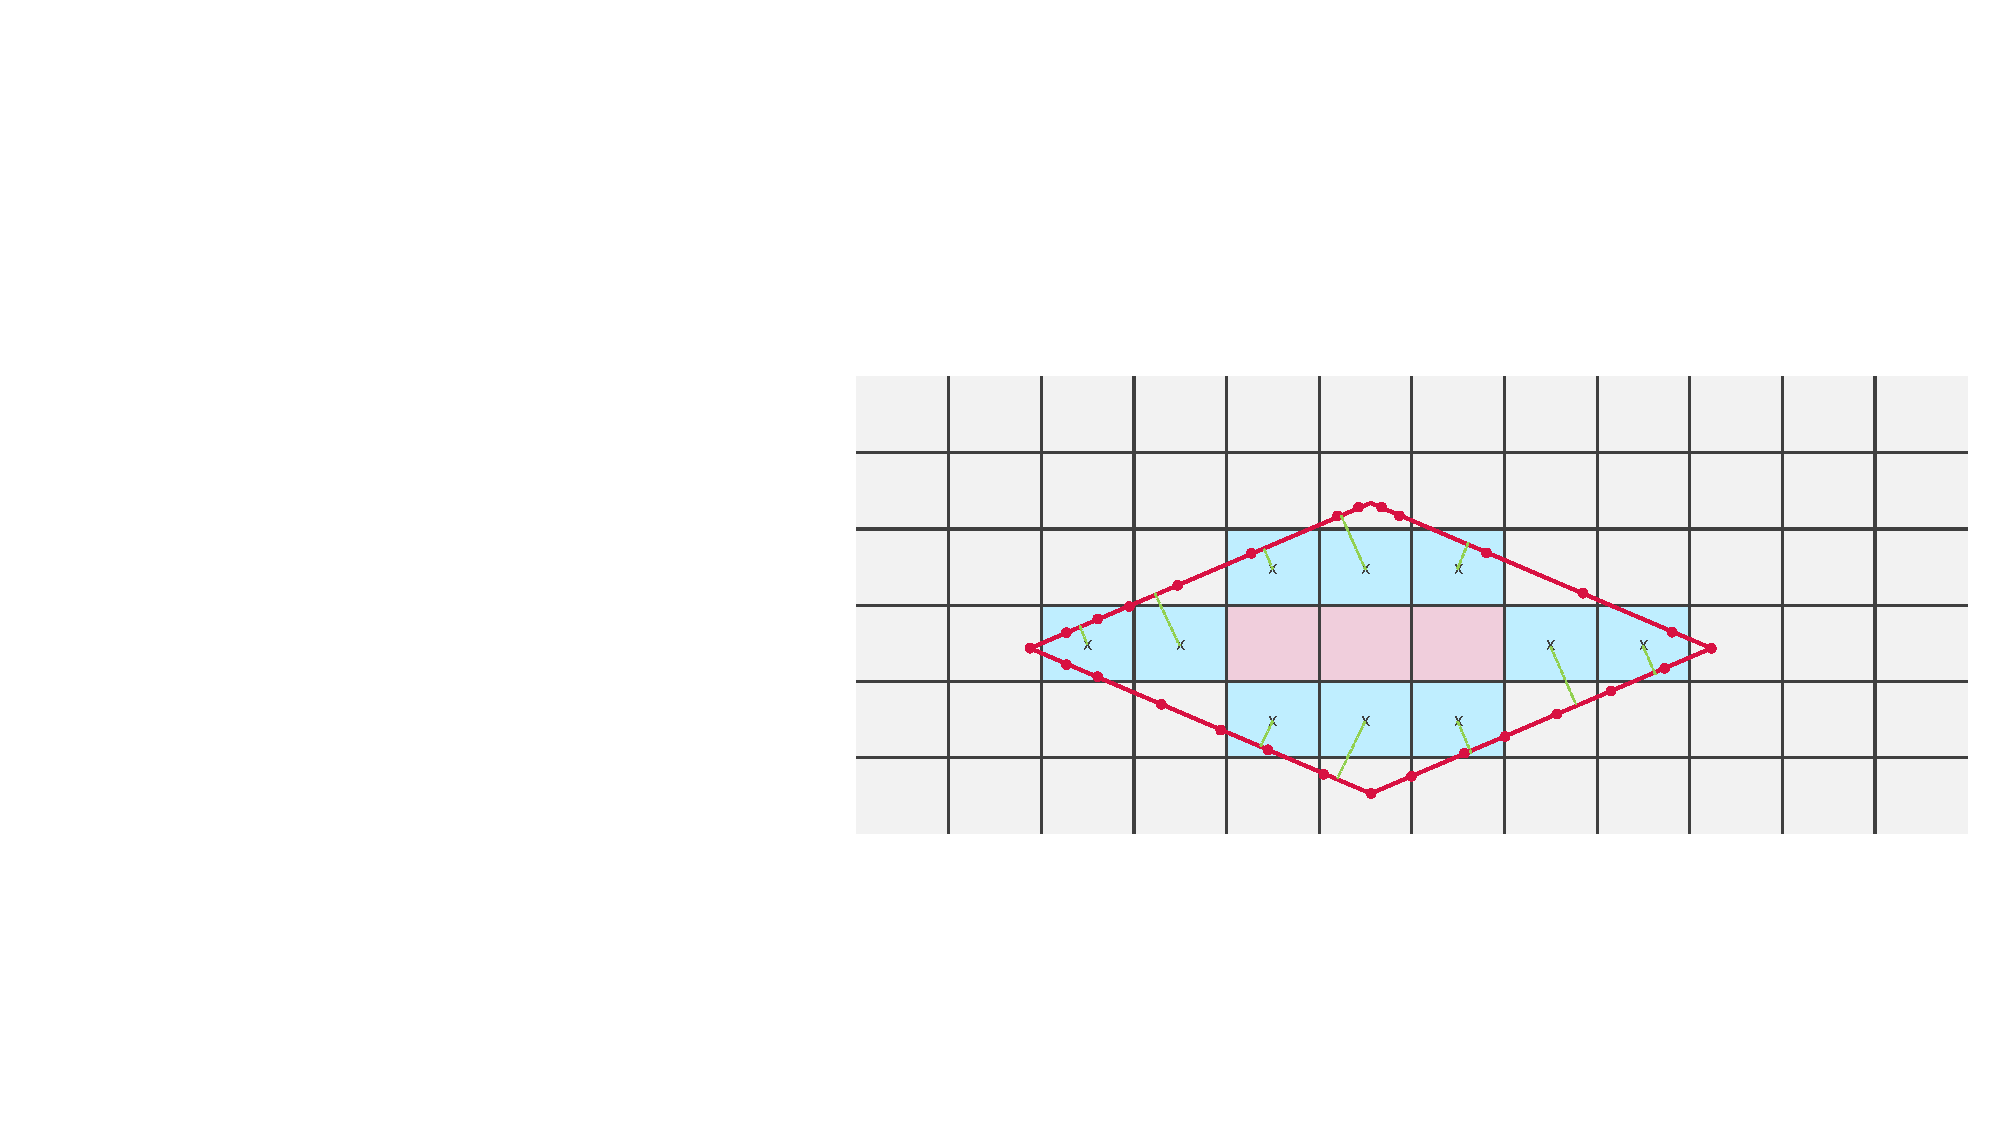
\includegraphics[width=0.3\linewidth]{chapter3_numerical_methods/pictures/ibm4.pdf} &
        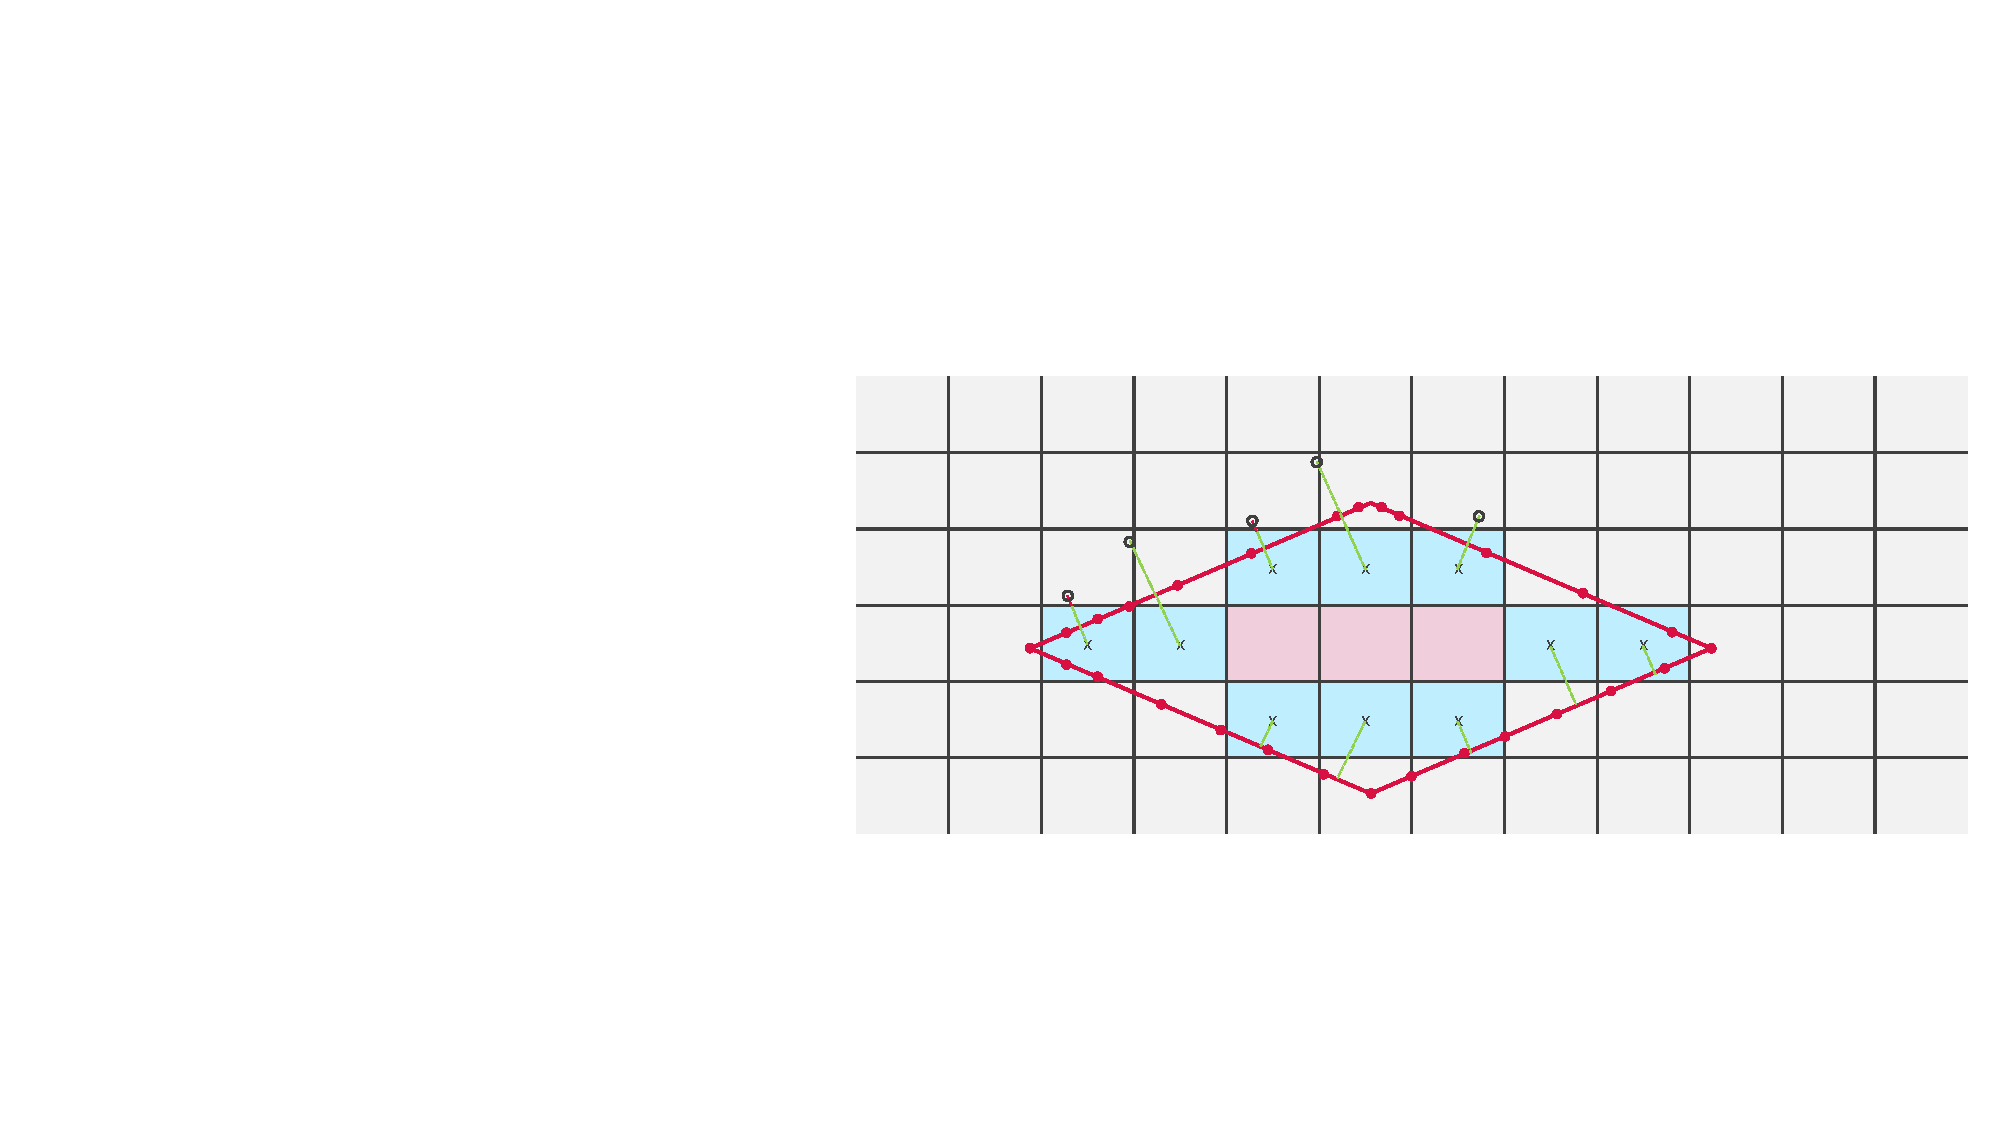
\includegraphics[width=0.3\linewidth]{chapter3_numerical_methods/pictures/ibm5.pdf} &
        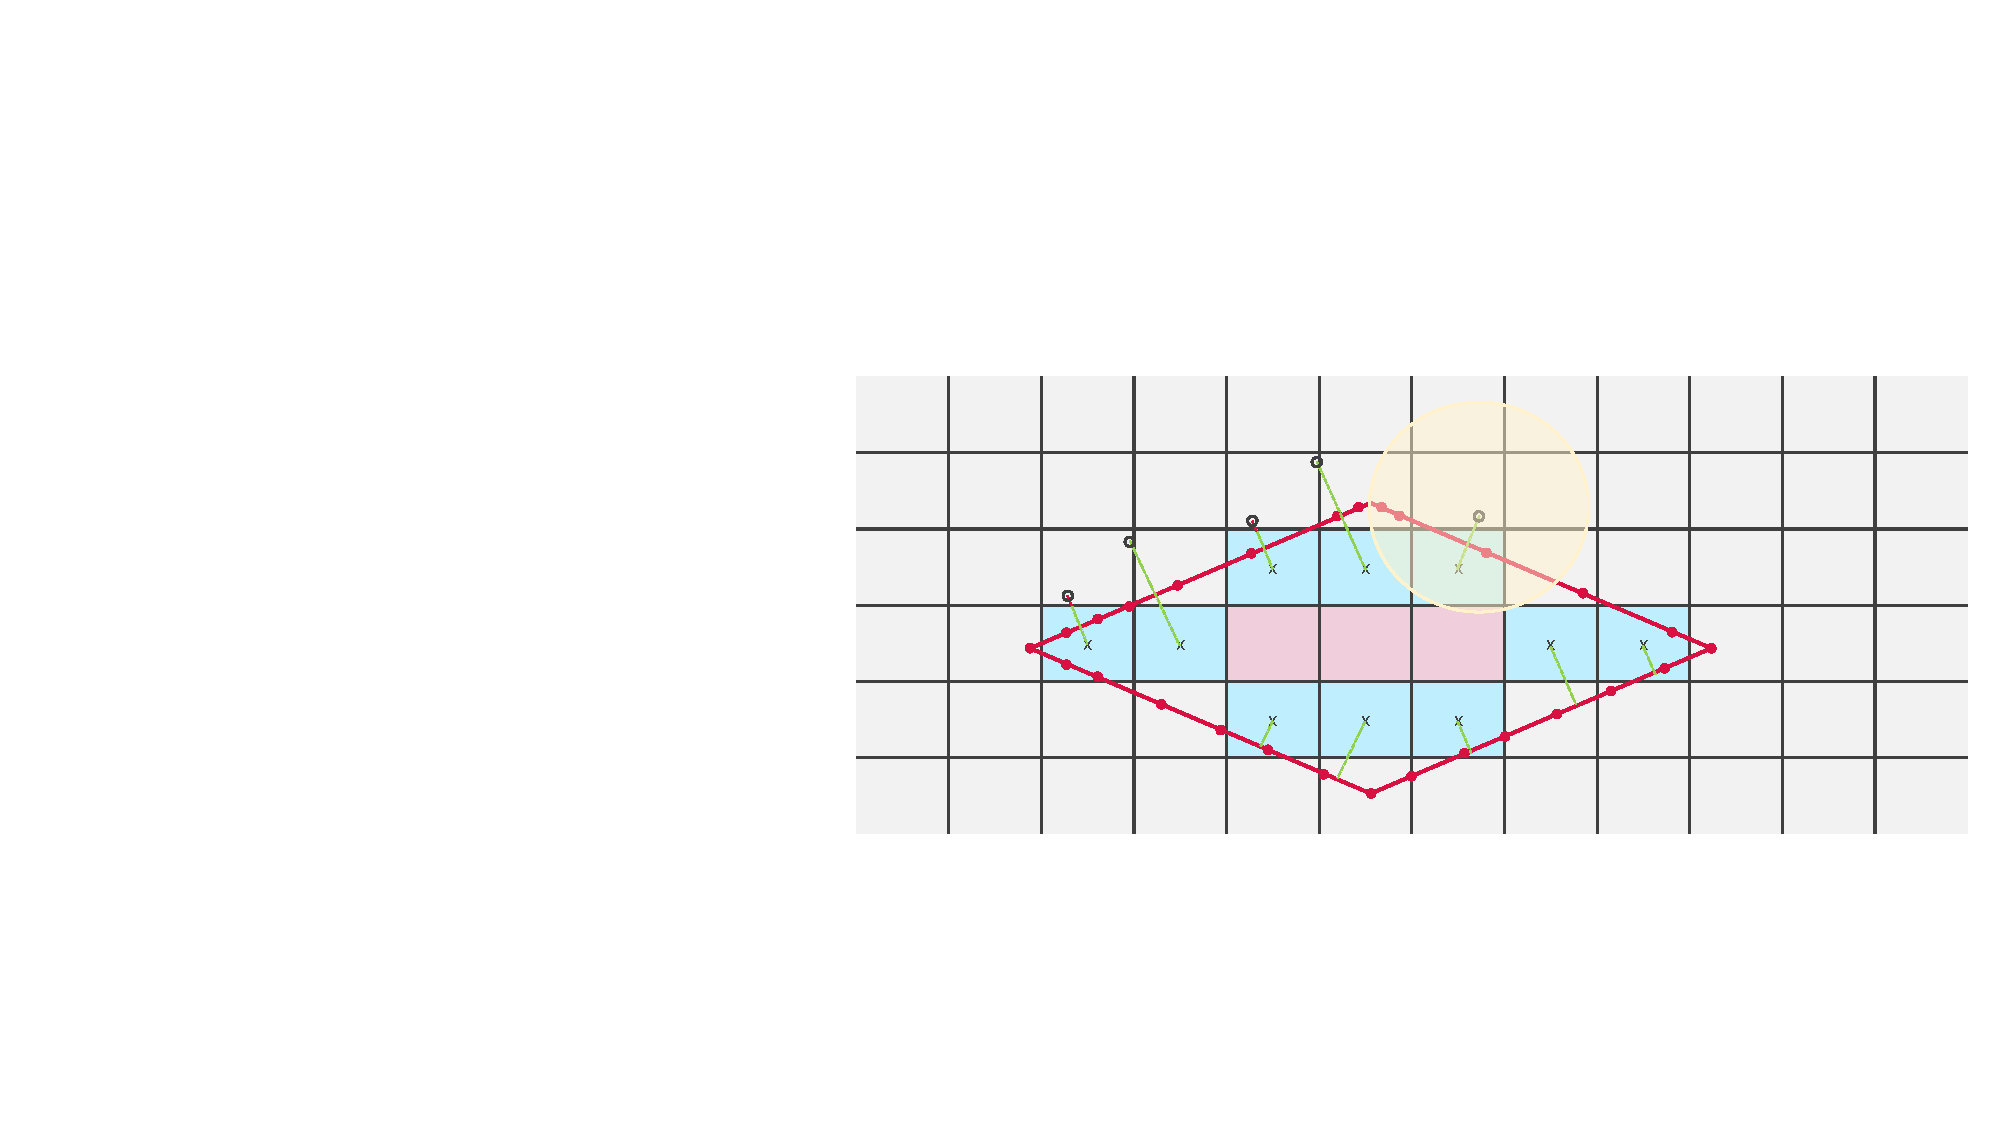
\includegraphics[width=0.3\linewidth]{chapter3_numerical_methods/pictures/ibm6.pdf} \\
        (d) & (e) & (f) \\
        & 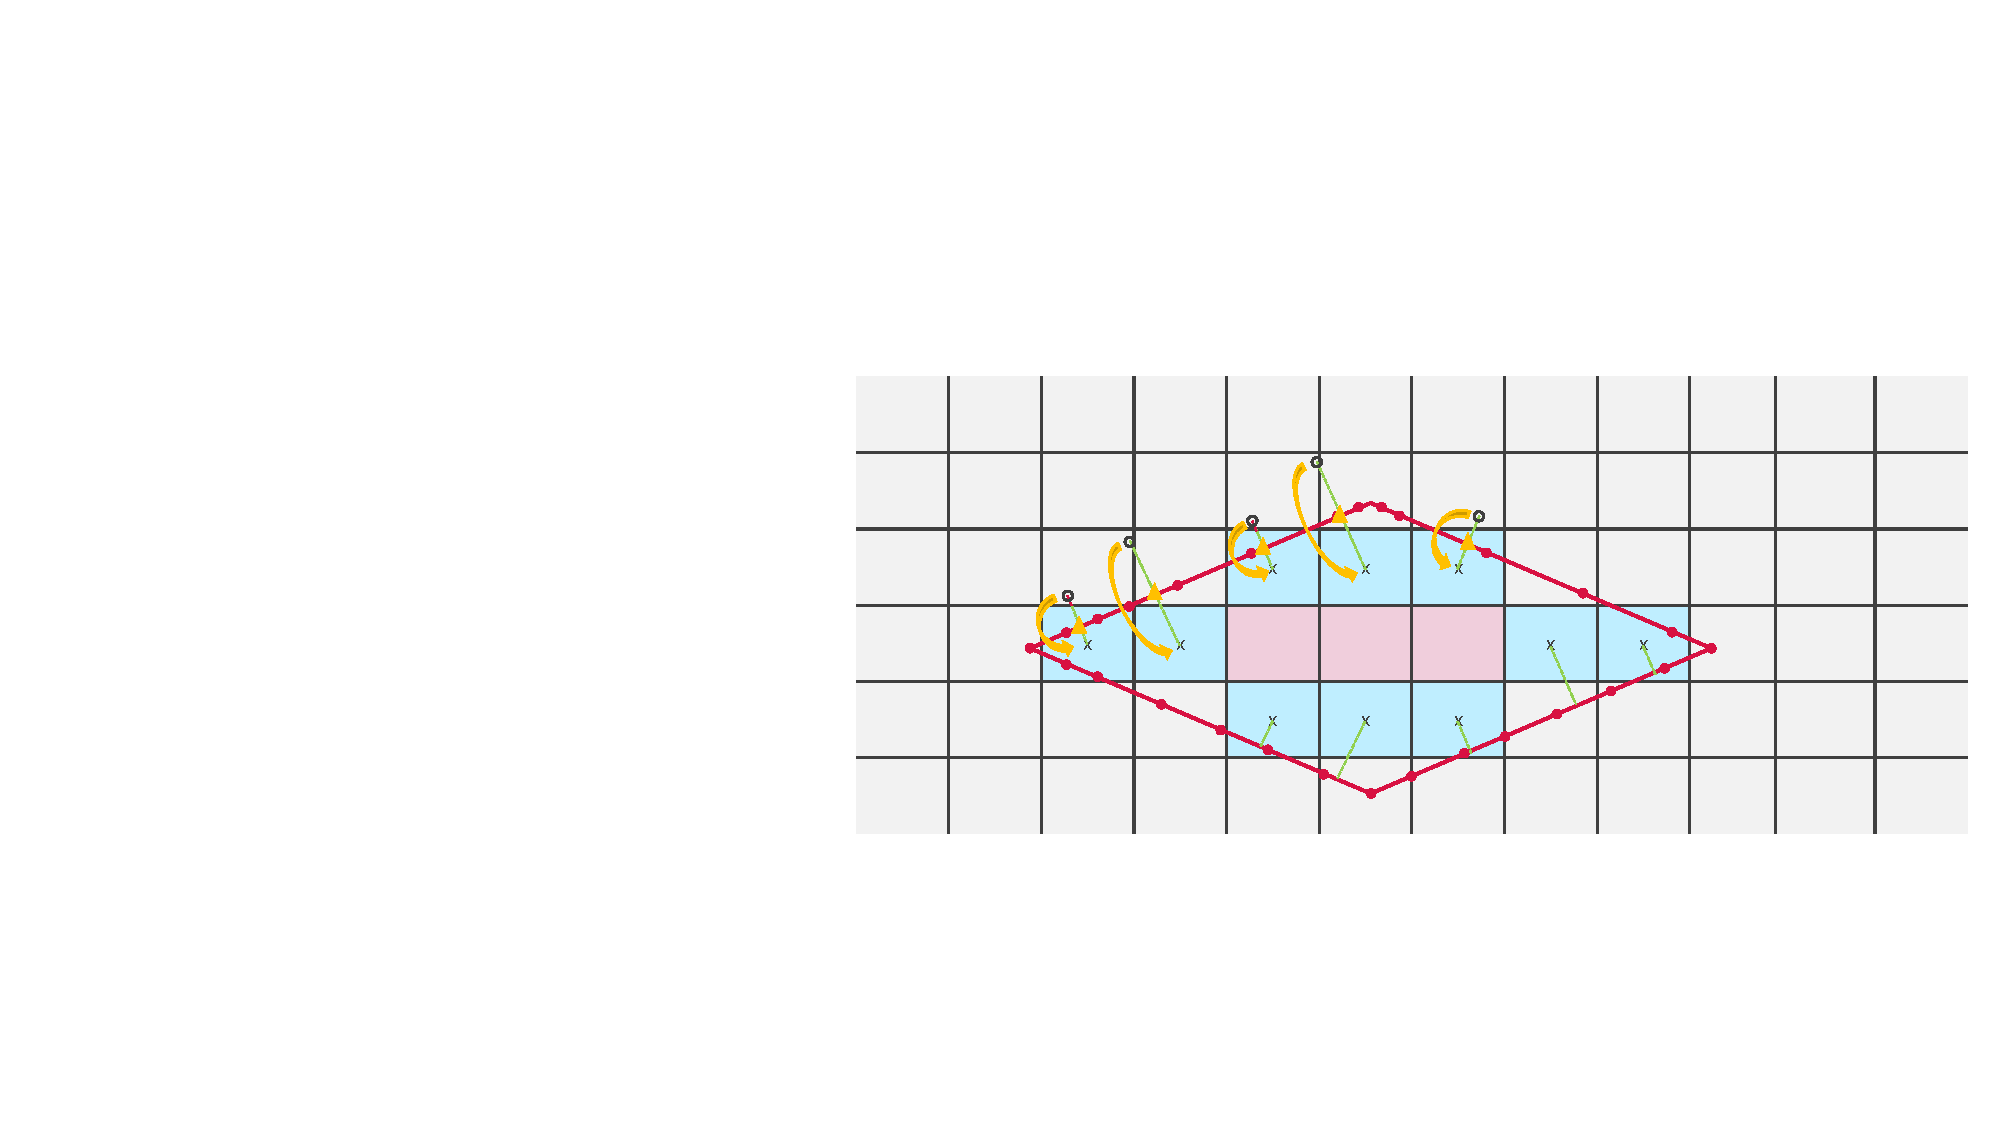
\includegraphics[width=0.3\linewidth]{chapter3_numerical_methods/pictures/ibm7.pdf} & \\
        & (g) &
    \end{tabular}
    \caption{Immersed boundary method workflow - diagrams are shown in two dimensions but the extension to three dimensions in straightforward.
    (a) Introduction of a tesselated object in the Cartesian mesh.
    (b) Detection of the immersed cells (red), $\emph{i.e.}$ solid cells, at initialization.
    (c) Detection of the immersed boundary cells (blue), $\emph{i.e.}$ solid cells with at least one fluid neighbor within the extent of the stencil, at initialization.
    (d) Detection of the nearest facet to each immersed boundary cell, at initialization
    (e) Creation of the image points in the direction normal to the nearest facet for each immersed boundary cell, at initialization.
    (f) Illustration of the neighborhood (yellow) where fluid cells are queried for information to interpolate the values of the fields at the image points, at each iteration of the fluid solver.
    (g) Illustration of the linear extrapolation from the image points to the immersed boundary cells to fill the values allowing for the enforcement of the boundary condition at the wall of the immersed object, at each iteration of the fluid solver.}
    \label{fig:ibm_workflow}
\end{figure}

To handle the presence of obstacles in the compressible flows, HYPERION uses a sharp immersed boundary method (IBM) \cite{mittal2005immersed}.
As mentioned in many papers, \emph{e.g.} \cite{khalili2019,qu2018}, the sharp interface method proves to be well suited for compressible flows because the boundary conditions at the immersed boundary are taken into account directly rather than being computed indirectly \emph{via} a forcing term or smoothed with a distribution function.
Originally, to handle boundary conditions at the edges of the domain, HYPERION uses ghost cells so there is no need to degenerate the reconstruction stencils at the edges.
To make use of the original data structures and logic of implementation as much as possible, we implemented a ghost-cell based immersed boundary method as well.
In the present study, we assume that the immersed objects cannot move.

We will briefly introduce in this section the workflow for the initialization of the immersed boundary method as it will serve as reference for future sections~\ref{sec:rasterization} and~\ref{sec:migratable_tasks}.
Overall the workflow is fairly classical \cite{mittal2005immersed,chi2017improved,khalili2019,qu2018,yousefzadeh2019,zhang2019} and relies on six main steps:

\begin{itemize}
    \item detection of the immersed cells, \emph{i.e.} all the cells of the Cartesian mesh that find themselves \emph{inside} the immersed object - figure~\ref{fig:ibm_workflow}(b),
    \item detection of the immersed boundary cells, that is immersed cells with at least one fluid neighbor within the extent of the reconstruction stencil, and wherein we shall impose the right values to enforce the boundary condition at the wall of the immersed object - figure~\ref{fig:ibm_workflow}(c),
    \item detection of the nearest facet to each immersed boundary cell in the sense of normal projection distance - figure~\ref{fig:ibm_workflow}(d),
    \item computation of the images of each immersed boundary cell center with respect to their nearest facet - figure~\ref{fig:ibm_workflow}(e),
    \item interpolation of the fluid variables at the image points - figure~\ref{fig:ibm_workflow}(f),
    \item linear extrapolation from the image points to the immersed boundary cells to enforce the boundary condition at the wall of the immersed object - figure~\ref{fig:ibm_workflow}(g).
\end{itemize}

In HYPERION, since we assume that all immersed objects are immovable, the four first steps can be done once during the initialization of the computation, whereas the last two steps, depending on the instantaneous state of the fluid, are repeated at each fluid iteration.

Section~\ref{sec:rasterization} will present the novel algorithm used in HYPERION to make the detection of the immersed cells (step 1) particularly inexpensive, even for three-dimensional objects and Cartesian meshes.
Step 2 and 4 are quite straightforward and rely on simple geometrical notions ; to make step 3 efficient however for large Cartesian meshes and finely discretized immersed objects, HYPERION builds a spatial-median Bounding Volume Hierarchy (BVH) of the immersed objects to accelerate the ray-tracing-like queries for nearest facets\footnote{"Find Closest Point on (Tesselated) Surface" library developed by \emph{ingowald} as a spin-off of the OSPRay project - see \url{github.com/ingowald/closestSurfacePointQueries}}.
Step 5 relies on the ENO-like least-square interpolation algorithm developed by one of the authors \cite{BRIDELBERTOMEU2021}, and section~\ref{sec:migratable_tasks} shall detail the strategy implemented in HYPERION to handle the large interpolation neighborhood in a massive parallelism context.
Finally, step 6 is straightforward as well and the interested reader can find all the mathematical details in Bridel-Bertomeu \cite{BRIDELBERTOMEU2021}.

\section{A FAST RASTERIZATION ALGORITHM TO DETECT IMMERSED CELLS}\label{sec:rasterization}
%
% [TBB] Ici on pointe sur (quasiment) la première partie du workflow IBC évoquée précédemment & on décrit l'algo de rasterization
% en 3D basé sur des maillages tétrahédriques des objets immergés et l'équivalence entre ce que nous on appelle un maillage Cartésien
% homogène et ce que la communauté du jeu vidéo appelle un maillage de voxel.
% Il va falloir ressusciter d'une façon ou d'une autre l'ancien algo 3D brute-force pour pouvoir fournir des comparaisons en terme de
% temps de traitement.
%

To identify the solid cells, \emph{i.e.} the cells of the Cartesian mesh that are found \emph{inside} the immersed object, the most common algorithm is a somewhat brute-force ray-casting algorithm (see \emph{e.g} \cite{haines1994point,mittal2005immersed}) that can be described as follows.

\begin{figure}[ht!]
    \centering
    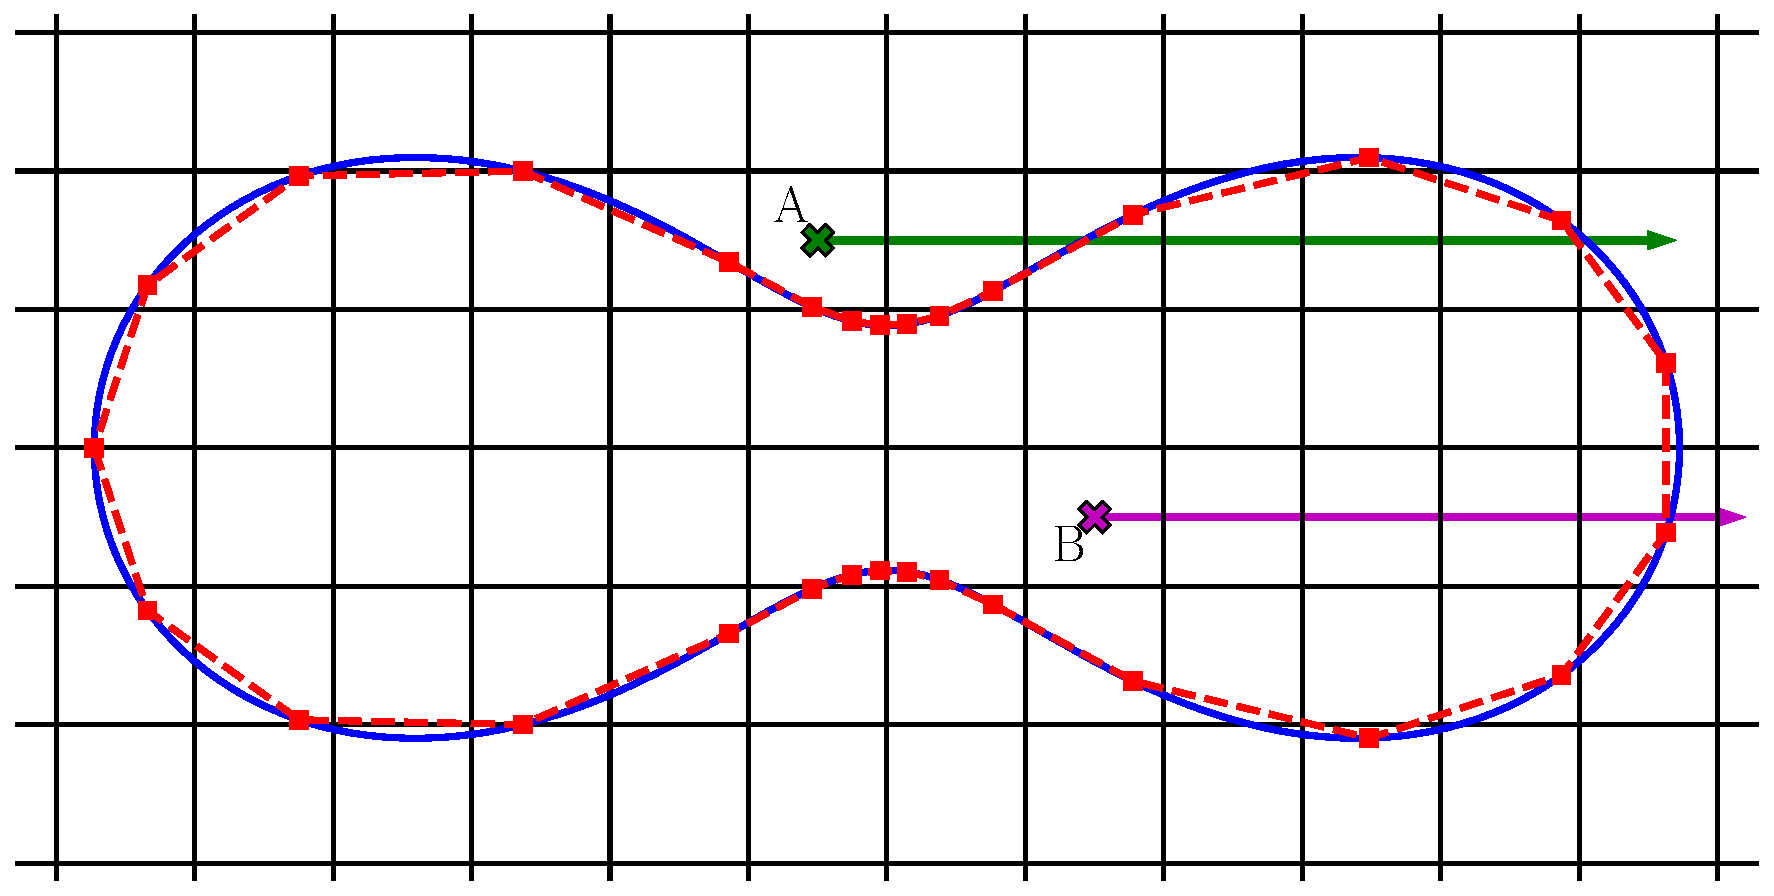
\includegraphics[width=0.7\linewidth]{chapter3_numerical_methods/pictures/cassini_ellipsis.pdf}
    \caption{Illustration of the tesselation of a two-dimensional curve and of the simple ray-casting algorithm for the identification of immersed cells.}
    \label{fig:ray_casting_simple}
\end{figure}

From all cells in the Cartesian mesh a random ray is cast (see for example cells $A$ and $B$ in figure~\ref{fig:ray_casting_simple}, but the ray could go any direction) and the intersections between this ray and the facets of the body are counted.
If the number of intersections is odd, then the cell wherefrom the ray is cast is inside the immersed body (for example cell $B$) whereas if the number of intersections is even, the originating cell is outside the immersed body (for example cell $A$).
The complexity of this algorithm is $\mathcal{O}\left( N_c N_f\right)$, where $N_c$ is the total number of cells in the Cartesian mesh and $N_f$ is the total number of facets of the tesselated immersed body. \\
For two-dimensional problems, such a complexity hardly becomes an issue.
As an illustration, let us nonetheless consider a three-dimensional worst case with a Cartesian mesh of $900 \times 900 \times 1300$ cells and an object with approximately $5\times 10^5$ facets, then the algorithm runs for more than $48$ hours on a mid-2017 Intel i7 processor with $4$ OpenMP threads.
Naturally if the Cartesian mesh is partitioned, then each partition handles its own set of rays and the time-to-completion drops to the order of magnitude of tens of minutes, but it still is not a reasonable performance - especially if one thinks of the possibility of having a moving object, for which the solid cells might change at each iteration of the fluid solver.

The technical name of the "problem that consists in finding the solid cells" is \emph{point classification}: in our case, we want to classify the cell centers according to whether they are inside or outside some shell.
\emph{Point classification} problems fall within the theory of computational geometry, which pushed the second author to associate himself with David Eberly \cite{schneider2002geometric} from Geometric Tools\footnote{See \url{https://www.geometrictools.com} for more information about the company} to develop a better algorithm than the aforementioned brute-force one - this section is dedicated to the presentation of this new algorithm.

The ray-casting algorithm simply needs the immersed object to be defined by the discretization of its outermost shell - a segment-based tesselation in two dimensions or a triangle-based tesselation in three dimensions.
The new algorithm relies on a tesselation of the outermost shell \emph{and} on the existence of a tetrahedralization (triangulation) of the inside of the object in three (two) dimensions - this shift in paradigm is illustrated on figure~\ref{fig:object_discretization}.

\begin{figure}
    \centering
    \begin{tabular}{cc}
        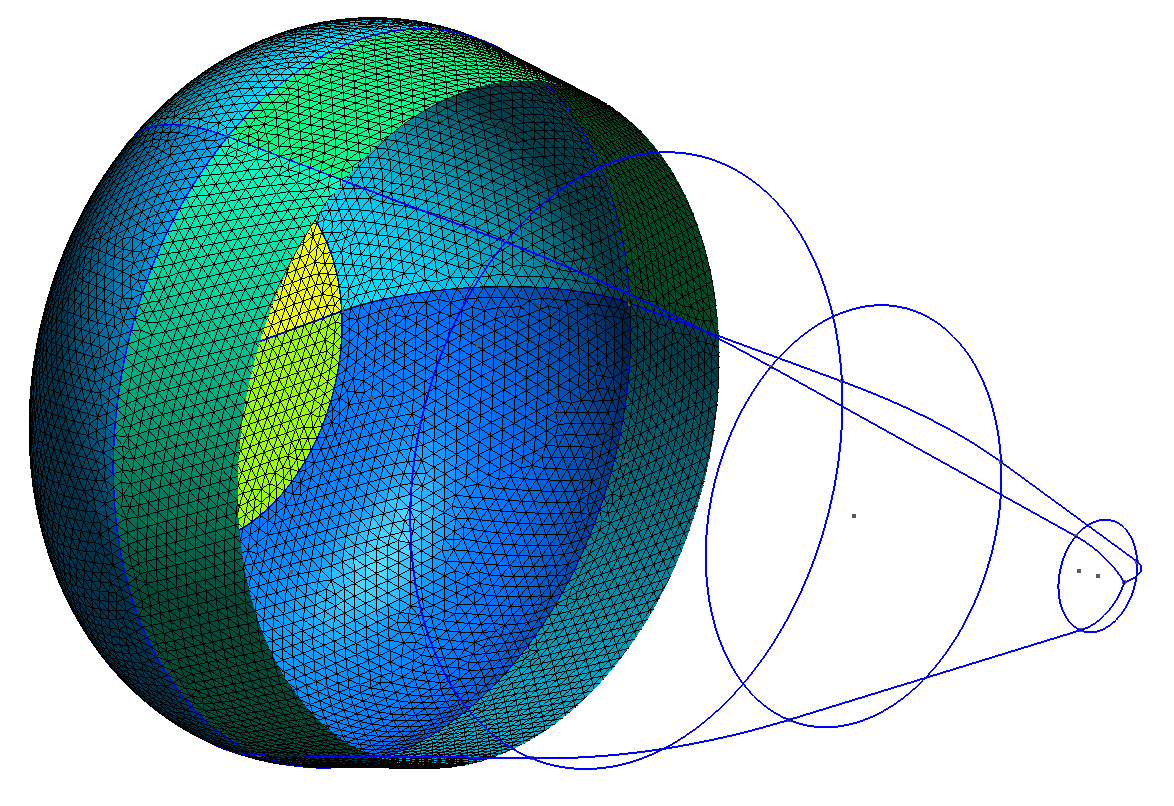
\includegraphics[width=0.45\linewidth]{chapter3_numerical_methods/pictures/funny_onion_shell.png} &
        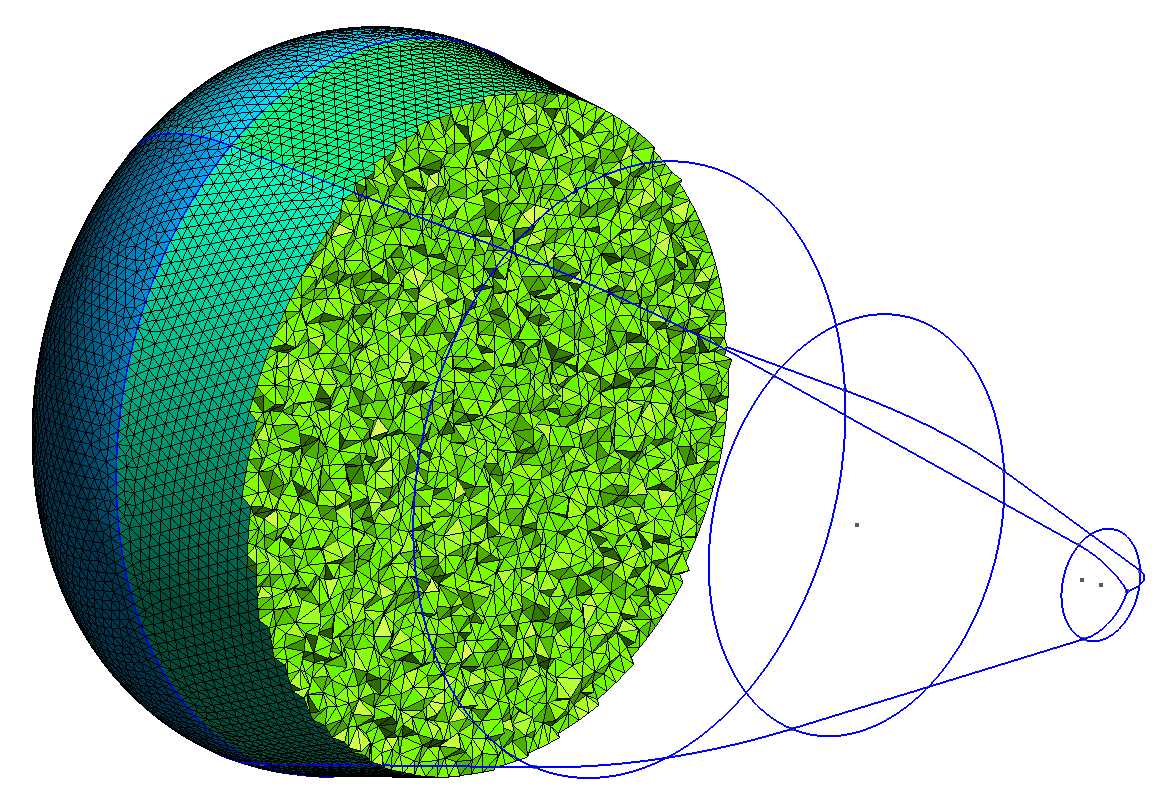
\includegraphics[width=0.45\linewidth]{chapter3_numerical_methods/pictures/funny_onion_threeD.png} \\
        (a) & (b)
    \end{tabular}
    \caption{Discretization of the immersed objects necessary (a) for the simple ray-casting algorithm and (b) for the new \emph{point classification} algorithm.
    The three-dimensional tetrahedralization required by the new algorithm has to be generated beforehand and is not handled by HYPERION.}
    \label{fig:object_discretization}
\end{figure}

Once a proper tetrahedralization (triangulation) has been obtained, the algorithm has the following steps - note that a description is provided in the three-dimensional case but the algorithm applies similarly in two dimensions.

\begin{itemize}
    \item[$\bullet$] Step 1 - for each tetrahedron, create its smallest axis-aligned bounding box (AABBs).

\begin{verbatim}
        function compute tetrahedra AABB
            for each tetrahedron t
                v1, v2, v3, v4 := the four vertices of the t
                t_min := v1
                t_max := t_max
                for each vertex v
                    for each dimension d
                        if coordinate d of v < coordinate d of t_min
                        then
                            coordinate d of t_min := coordinate d of v
                        else if coordinate d of v > coordinate d of t_max
                        then
                            coordinate d of t_max := coordinate d of v
                        end if
                    end for each
                end for each
            end for each
        end function
\end{verbatim}

    \item[$\bullet$] Step 2 - each AABB is clipped/culled against the underlying Cartesian mesh to ensure that when searching within the bounding boxes, the grid points are within range of the Cartesian mesh bounds. Note that the "underlying Cartesian mesh" can very well be a local piece of mesh in the context of MPI partitioning, making this \emph{point classification} inherently adapted to distributed parallelism.

\begin{verbatim}
        function cull tetrahedra AABB
            m_min, m_max := lower, upper vertex of Cartesian box
            for each tetrahedron t
                t_min, t_max := lower, upper vertex of t bounding box
                for each dimension d
                    coordinate d of t_min :=
                        max between
                            | coordinate d of t_min,
                            | coordinate d of m_min
                    coordinate d of t_max :=
                        min between
                            | coordinate d of t_max,
                            | coordinate d of m_max
                    if coordinate d of t_min > coordinate d of t_max
                    then
                        declare t invalid
                    end if
                end for each
            end for each
        end function
\end{verbatim}

    \item[$\bullet$] Step 3 - the tetrahedra vertices and bounding boxes are then transformed to the $(i,j,k)$ grid coordinate system.

\begin{verbatim}
        function transform to grid ijk
            m_min, m_max := lower, upper vertex
                of Cartesian box
            n.0, n.1, n.2 := number of cells
                of Cartesian box in each dimension
            for each dimension d
                factor.d := (n.d - 1) / (
                    coordinate d of m_max -
                    coordinate d of m_min
                )
            end for each
            for each tetrahedron t
                t_min, t_max := lower, upper vertex
                    of t bounding box
                for each dimension d
                    g_t_min := ceiling of factor.d * (
                        coordinate d of t_min -
                        coordinate d of m_min
                    )
                    g_t_max := floor of factor.d * (
                        coordinate d of t_max -
                        coordinate d of m_min
                    )
                end for each
            end for each
        end function
\end{verbatim}

    \item[$\bullet$] Step 4 - each grid-coordinate bounding box contains a relatively small number of the Cartesian grid cell centers, hence we can iterate over those with a triple loop in $k$, then $j$, then $i$ as per HYPERION grid ordering. For a constant $(j,k)$ in the grid box, a line segment containing cell centers with varying $i$ is obtained. Note that one possible implementation of the function determining whether a point is in a tetrahedron can be found in \cite{schneider2002geometric} and shall not be repeated here.

\begin{verbatim}
    function rasterize
        n.0, n.1, n.2 := number of cells
            of Cartesian box in each dimension
        for each tetrahedron t
            g_t_min, g_t_max := lower, upper vertex
                of t bounding box in ijk coordinates
            for k from g_t_min.2 to g_t_max.2
                for j from g_t_min.1 to g_t_max.1
                    for i0 from g_t_min.0 to g_t_max.0
                        if (i0,j,k) in tetrahedron t
                        then
                            break for i0
                        end if
                    end for
                    if i0 > g_t_max.0
                    then
                        cycle for j
                    end if
                    for i from g_t_max.0 down to i0
                        if (i,j,k) in tetrahedron t
                        then
                            break for i
                        end if
                    end for
                    base := n.0 * (j + n.1 * k)
                    for l from i0 to i
                        n := l + base
                        flag cell center of index n
                            as inside tetrahedron t
                    end for
                end for
            end for
        end for each
    end function
\end{verbatim}

    \item[$\bullet$] Step 5 - the $i$-values are searched for the first and last cell centers that are inside each tetrahedron, if any, which yields a set of flagged $(i,j,k)$ that can be said to be inside the immersed object.
\end{itemize}

As mentioned, the algorithm can be easily adapted to a code working in parallel.
For a multithreaded code, then the tetrahedra can be split among the different threads to share the workload.
There is a chance that two threads might try to flag the same $(i,j,k)$ to the set of solid cells.
In particular this can happen if a cell center is on the shared face of a pair of tetrahedra (or close to that face because of numerical rounding errors).
However, there is no need for a critical section or an atomic write: first, from the perspective of either thread the cell center will be found to be inside the immersed object, and anyway the $(i,j,k)$ grid coordinates are $32$-bit integers that are written atomically by nature. \\
If the number of tetrahedra in the discretization of the object is noted $N_t$, then the complexity of this algorithm is, mostly, $\mathcal{O}(N_t)$.
For the same worst-case problem as before, the time-to-completion falls to $8.5$ seconds on a single OpenMP thread and the timings for $2$, $4$, $8$ and $16$ OpenMP threads are $4.3$ seconds, $2.6$ seconds, $2.1$ seconds and $2.0$ seconds respectively (versus $\gtrsim 48$ hours for the brute-force algorithm for $4$ OpenMP threads).

\section{MIGRATABLE TASKS FOR THE MASSIVE PARALLELIZATION OF THE RECONSTRUCTION ALGORITHM}\label{sec:migratable_tasks}

As mentioned in section~\ref{ssec:ibc}, the interpolation of the fluid values at each image point (step 5) relies on the least-square ENO-like interpolation discussed in details in the paper by Bridel-Bertomeu \cite{BRIDELBERTOMEU2021}.
A short study in the latter paper mentions that for the algorithm to be robust (\emph{i.e} for the least-square matrix to be well enough conditioned), at least 25 neighbors are necessary in two dimensions for a third order interpolation.
The same kind of study conducted in three dimensions shows that at least 85 neighbors are required for a third order interpolation so that the least-square matrix reaches its asymptotic minimum conditioning.

Furthermore, to balance the number of neighbors picked in each direction around the cell of interest, HYPERION implements a spiral walk (see \cite{BRIDELBERTOMEU2021}, figure~4(a)): with that strategy, getting to 25 (85) neighbors in two (three) dimensions means having access to at least three layers of cells around the cell of interest.
However, considering that such cells of interest are by nature in proximity to the immersed objects and because we cannot consider the immersed cells as valid neighbors in the interpolation, acquiring the information from enough valid neighbors can quickly lead to accessing the fifth or sixth layer of cells away from the cell of interest (\emph{e.g.} for fourth or fifth order interpolation matching the order of the TENO reconstruction described in paragraph~\ref{sssec:interpolations}).

In a sequential, or even in a shared-memory parallelism context, accessing cells that are far away from the cell of interest is not a challenge - the algorithm presented in \cite{BRIDELBERTOMEU2021} could be implemented directly without any modifications in a purely sequential or only OpenMP version of HYPERION.
In a distributed parallelism context however, things become rather tricky if one aims at minimizing the computational overhead related to communications between processes and/or the overall memory use of the application, as is the goal for HYPERION.

\begin{figure}[ht!]
    \centering
    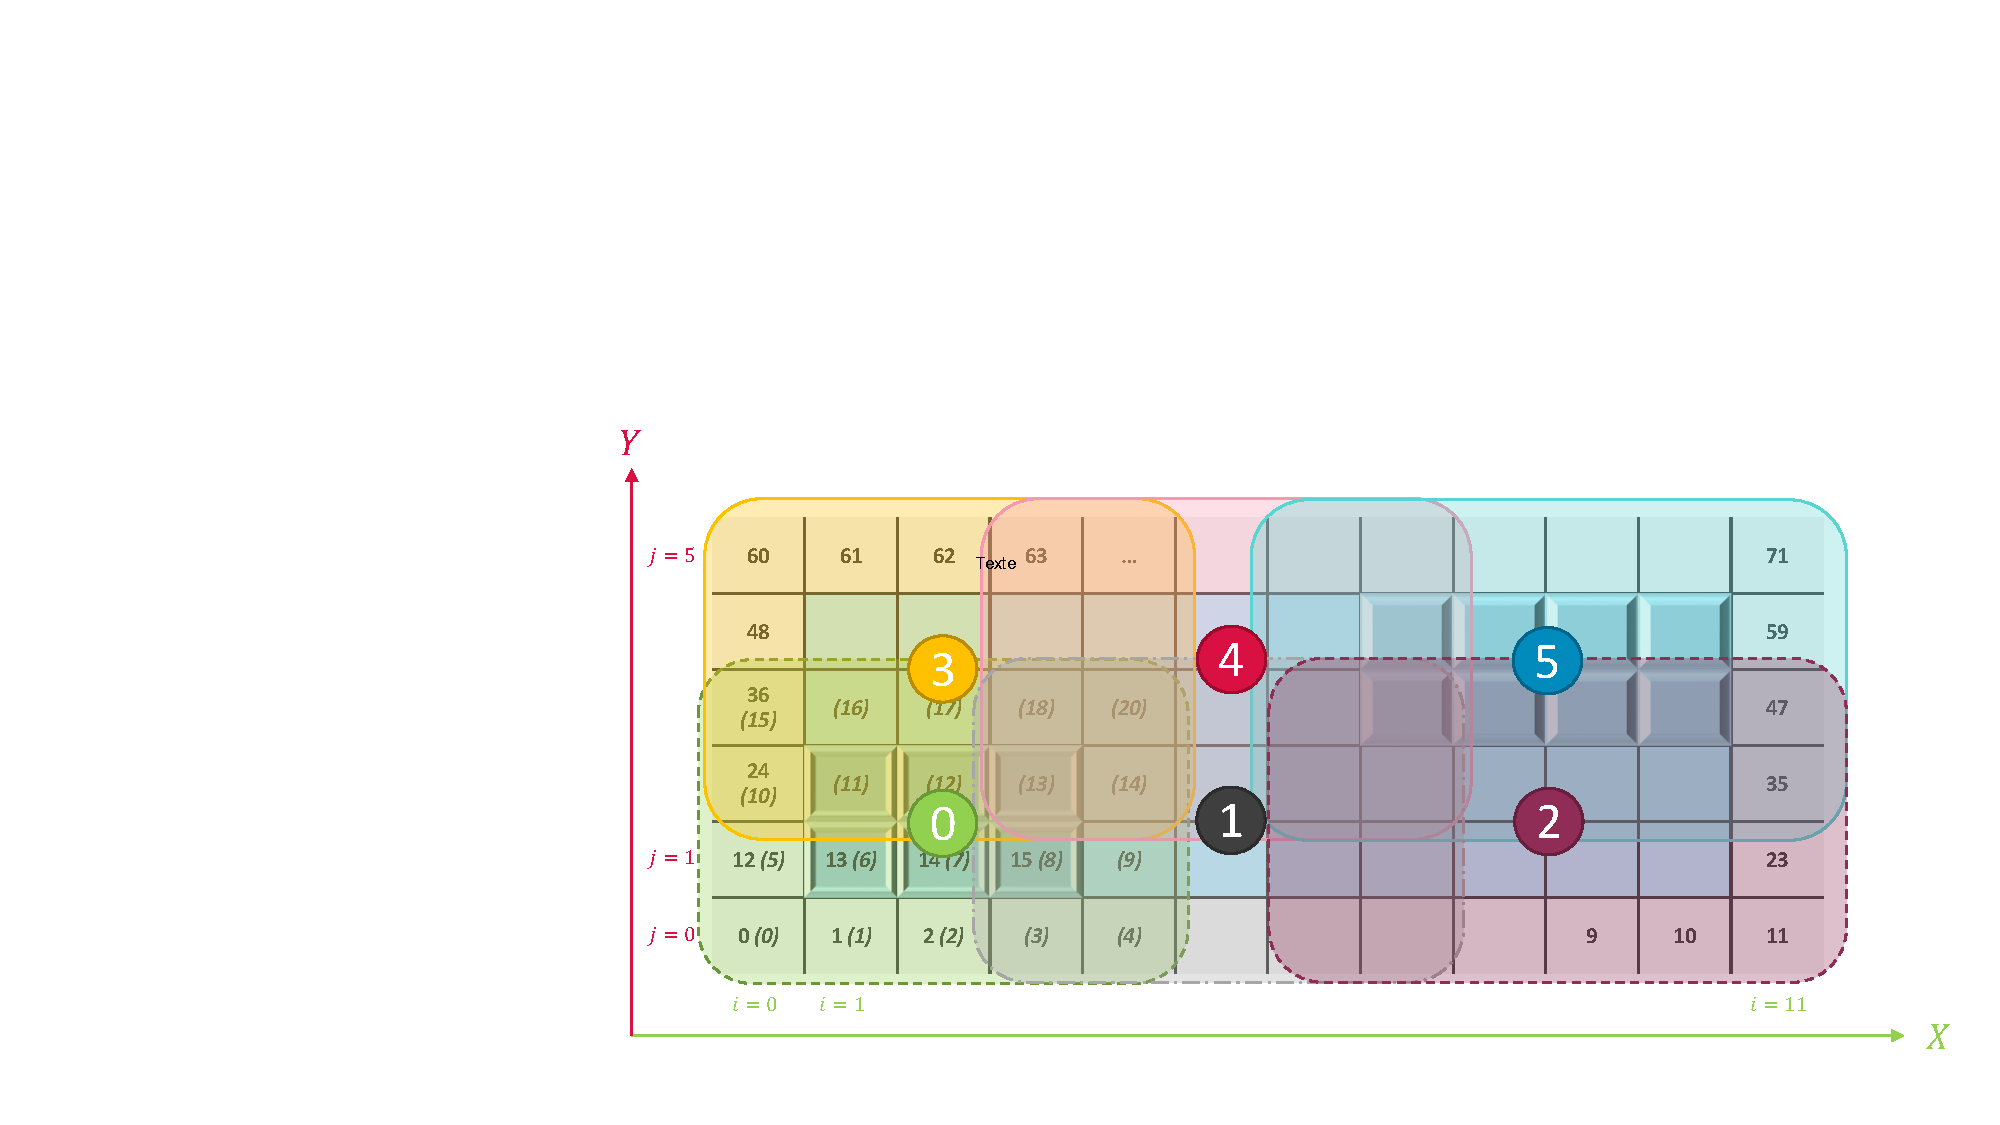
\includegraphics[width=0.75\linewidth]{chapter3_numerical_methods/pictures/mpi_halo.pdf}
    \caption{Illustration of the Cartesian partitioning of the Cartesian mesh in HYPERION.
    The overlapping halos (of size 1 in this case) ensuring communications between neighboring processes are also represented.
    Note that the numbering of the MPI processes is done the same way as the numbering of the fluid cells.}
    \label{fig:mpi_halos}
\end{figure}

If only in terms of memory use, note that out of consistency, in HYPERION the size of the MPI halo equals the number of ghost cells used at the edges of the domain - see figure~\ref{fig:mpi_halos}.
Therefore, if we consider a rather common mesh size of $512^3$ cells, and if we attempt to gain access to cells six layers away with a halo of size $6$, the actual mesh handled by HYPERION has size $(512 + 2 \times 6)^3$, which, if we only account for the five conservative variables, means an overhead of about $3$ Gi in memory.
HYPERION efficiency is around $1$ to $1.5$ $\mu$s$_{\text{CPU}}$/it/cell, hence using a size $6$ halo tends to introduce an overhead of about $10$ s$_{\text{CPU}}$ at each iteration.

With these considerations in mind, along with the fact that having \emph{e.g.} size $6$ halos is highly detrimental to the performance of the MPI communications (although it has not been quantitatively evaluated in the present study), we worked on an algorithm that would not rely on the MPI halos at all in order to perform well in conjunction with any kind of reconstruction stencil.
% that would perform well even with the tighter size $3$ halos required by the TENO reconstruction scheme.
Inspired by the spiral "walk" used in a sequential context to gather information from enough valid neighbors for the least-square interpolation, we turned ourselves towards a migratable task paradigm. \\
In this paradigm, the first ingredient is a \emph{task}.
In our context, let us remember that for each image point we want to gather information from enough "valid" neighbors to have a well-conditioned least-square matrix (see figures~\ref{fig:ibm_workflow}(f) and~\ref{fig:migratable_task}(a)).

\begin{figure}[ht!]
    \centering
    \begin{tabular}{cc}
        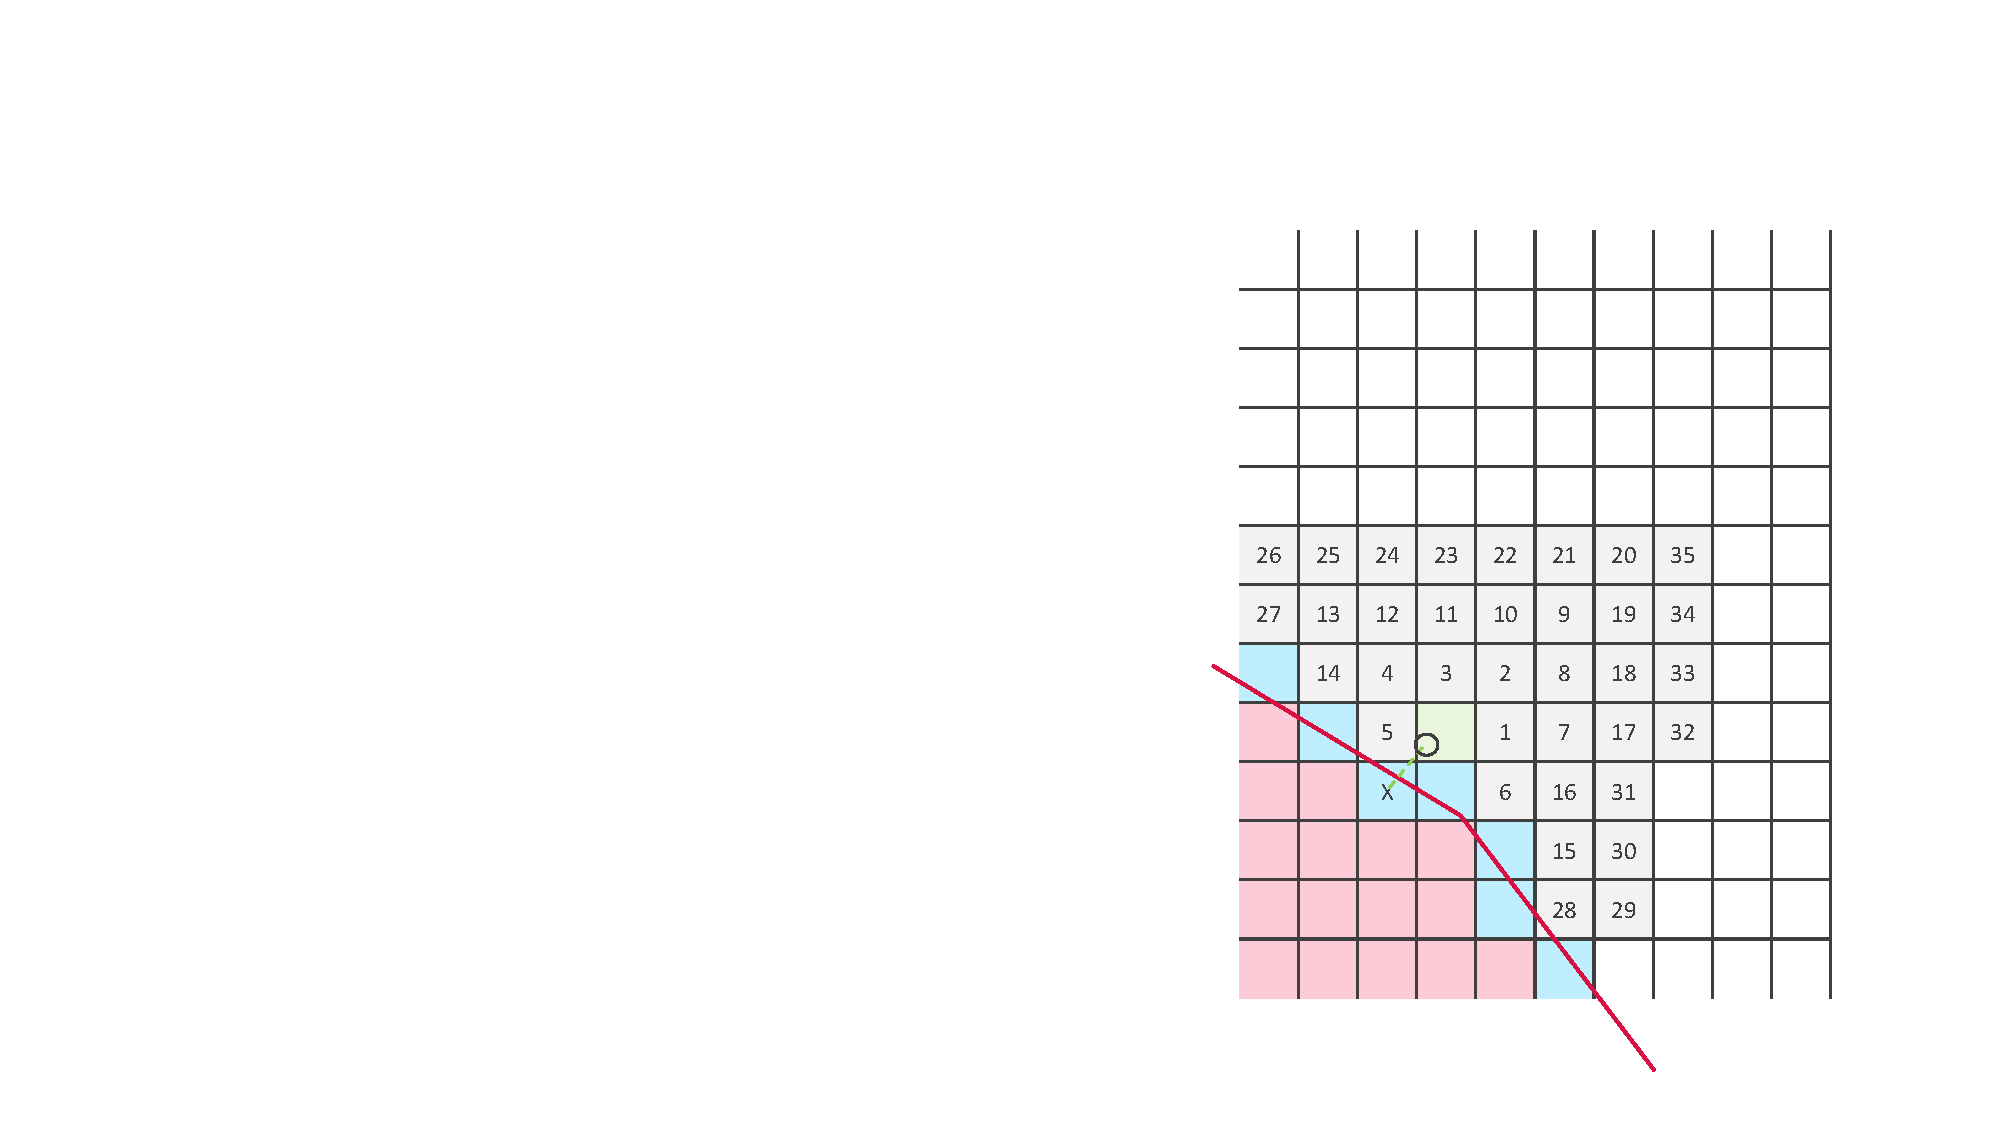
\includegraphics[width=0.35\linewidth]{chapter3_numerical_methods/pictures/BC_migrable1.pdf} &
        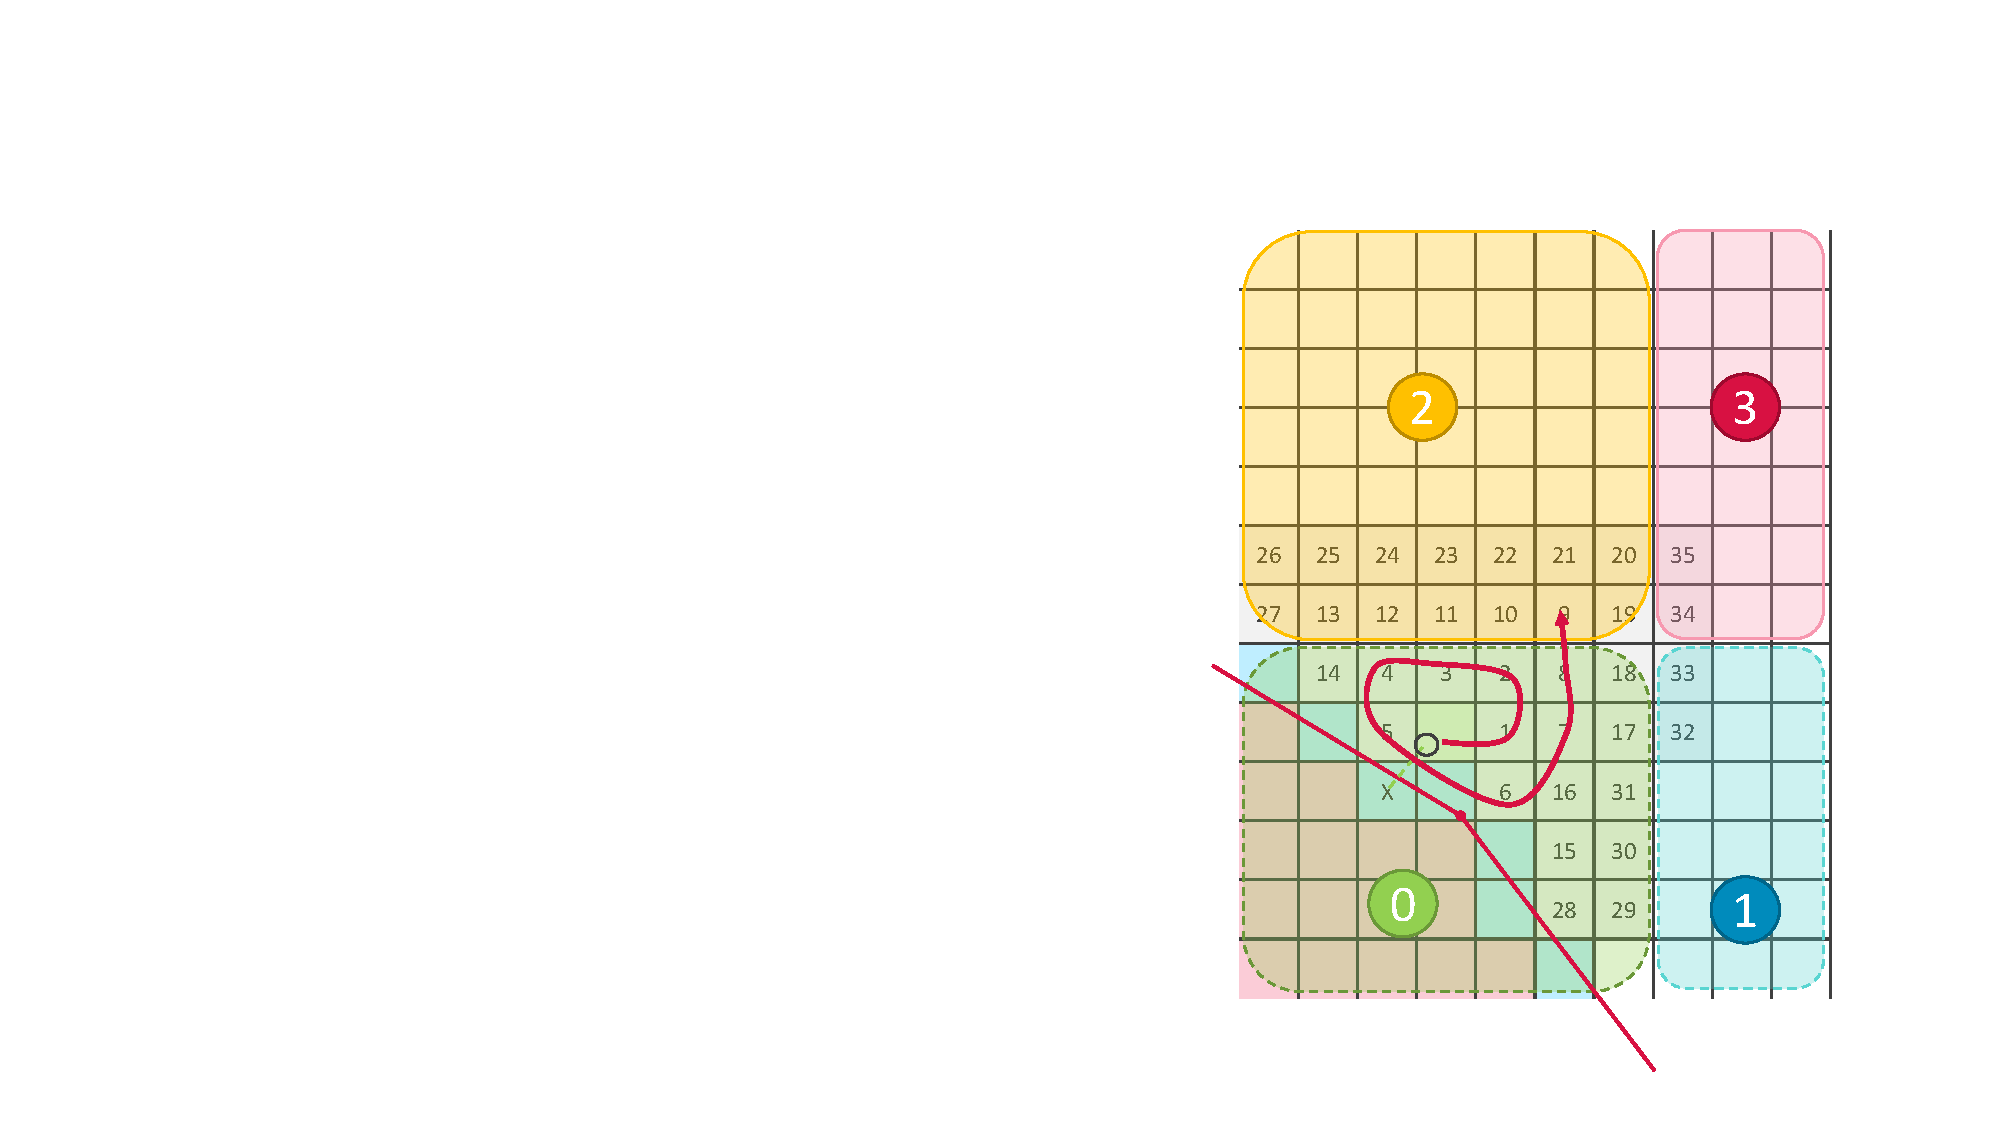
\includegraphics[width=0.35\linewidth]{chapter3_numerical_methods/pictures/BC_migrable2.pdf} \\ [0.5em]
        (a) & (b)
    \end{tabular}
    \caption{(a) Zoom on the neighborhood of an immersed boundary cell image and the corresponding surrounding cells numbering for the spiral walk.
    (b) Illustration of the spiral walk task in the migratable task algorithm and of the influence of partitioning thereupon - the halos are omitted as the algorithm does not make use of them.}
    \label{fig:migratable_task}
\end{figure}

To do so, we emit a probe that will march the surrounding cells in a spiral motion: for each "valid" neighbor (that is not an immersed cell), the index of the cell and the values of the fluid variables are stored in the probe structure before it goes on.
This marching is the \emph{task} in the migratable task paradigm - see figure~\ref{fig:migratable_task}(b) - which is supported by a simple data structure:

\begin{verbatim}
struct _probe_task_state
    status  // status of the marching
    (x,y,z) // current coordinate of the head of the probe

    coords[] // coordinates of valid neighbors, accumulated
    values[] // fluid variables in the valid neighbors, accumulated

    origin_rank // rank of the processes wherefrom the probe originates
    rank // rank of the process the probe needs to be sent to, if any

    count // current number of neighbors
end struct
\end{verbatim}

Because of the partitioning of the Cartesian mesh, several, if not all, processes own immersed boundary cells and must therefore emit probes.
In terms of implementation, each process has a stack of such tasks that it works through either sequentially or in parallel with multiple shared-memory OpenMP threads.
During its march, if a probe next step has to be taken on a different process (illustrated on figure~\ref{fig:migratable_task}(b)), then a message is sent from its current owner to the neighboring process containing the entire probe structure ; in so doing, the probe is popped from the previous owner stack of tasks and pushed to the neighbor process stack that can resume the walk of the probe.
This march of each probe continues until it has found enough valid neighbors, \emph{per} the user request, at which point the whole structure of the probe is sent back to the process it originated from so the least-square interpolation can take place and the immersed boundary cell can be populated with values enforcing the immersed boundary condition \cite{BRIDELBERTOMEU2021}.

Note that during the course of the algorithm, no process can predict with simple logic whether it is going to receive a task from a neighbor or whether it will have to send one of its tasks to a neighbor - since no process knows whether to expect a message, they all wait for messages asynchronously while handling the tasks on their stacks.
This poses a well-known problem in parallel computations, namely a termination issue.
Since no process knows to expect a message, if nothing is done all the processes will eventually finish working on their own tasks and wait indefinitely for messages from their neighbors.
To prevent such an infinite loop from occurring in HYPERION, we implemented the algorithm of Francez \emph{et al.} \cite{francez1982} to achieve distributed termination without introducing any new communication.

The entire pseudocode algorithm is described below.

\begin{verbatim}
while not terminated
    %MASTER THREAD
    {
        while to_send_stack not empty
            e := pop to_send_stack
            async send e to e.rank
            sent_stack push e
        end while
        while sent_stack not empty
            check sent request has gone through
        end while
        probe all sources for any message
        if message
            new_e := deserialize message
            stack push new_e
        end if
        terminated ?= francez termination algorithm
    }
    %END MASTER THREAD
    while stack not empty
        e := pop stack
        until enough neighbors
            go to the next cell in the spiral
            if next cell is solid or ghost
            then
                skip
            else
                if next cell on current process
                    e.coords append cell center coordinates
                    e.values append cell values
                    increment e.count
                    if enough neighbors
                        e.status := SUCCESS
                        break until
                    end if
                else
                    e.rank := neighbor rank
                    break until
                end if
            end if
        end until
        if e.status == SUCCESS
            e.rank := e.origin_rank
        end if
        if e.status == SUCCESS and current process rank == e.origin_rank
            solve least square problem
            compute immersed ghost cell value
        else
            to_send_stack push e
        end if
    end while
end do
\end{verbatim}

This migratable task strategy allowed us to use the ENO-like interpolation algorithm with large neighborhoods in massively parallel computations with guaranteed stability, yielding a satisfactory speed-up up to $4096$ processes as shown on figure~\ref{fig:speed_up}.

\begin{figure}
    \centering
    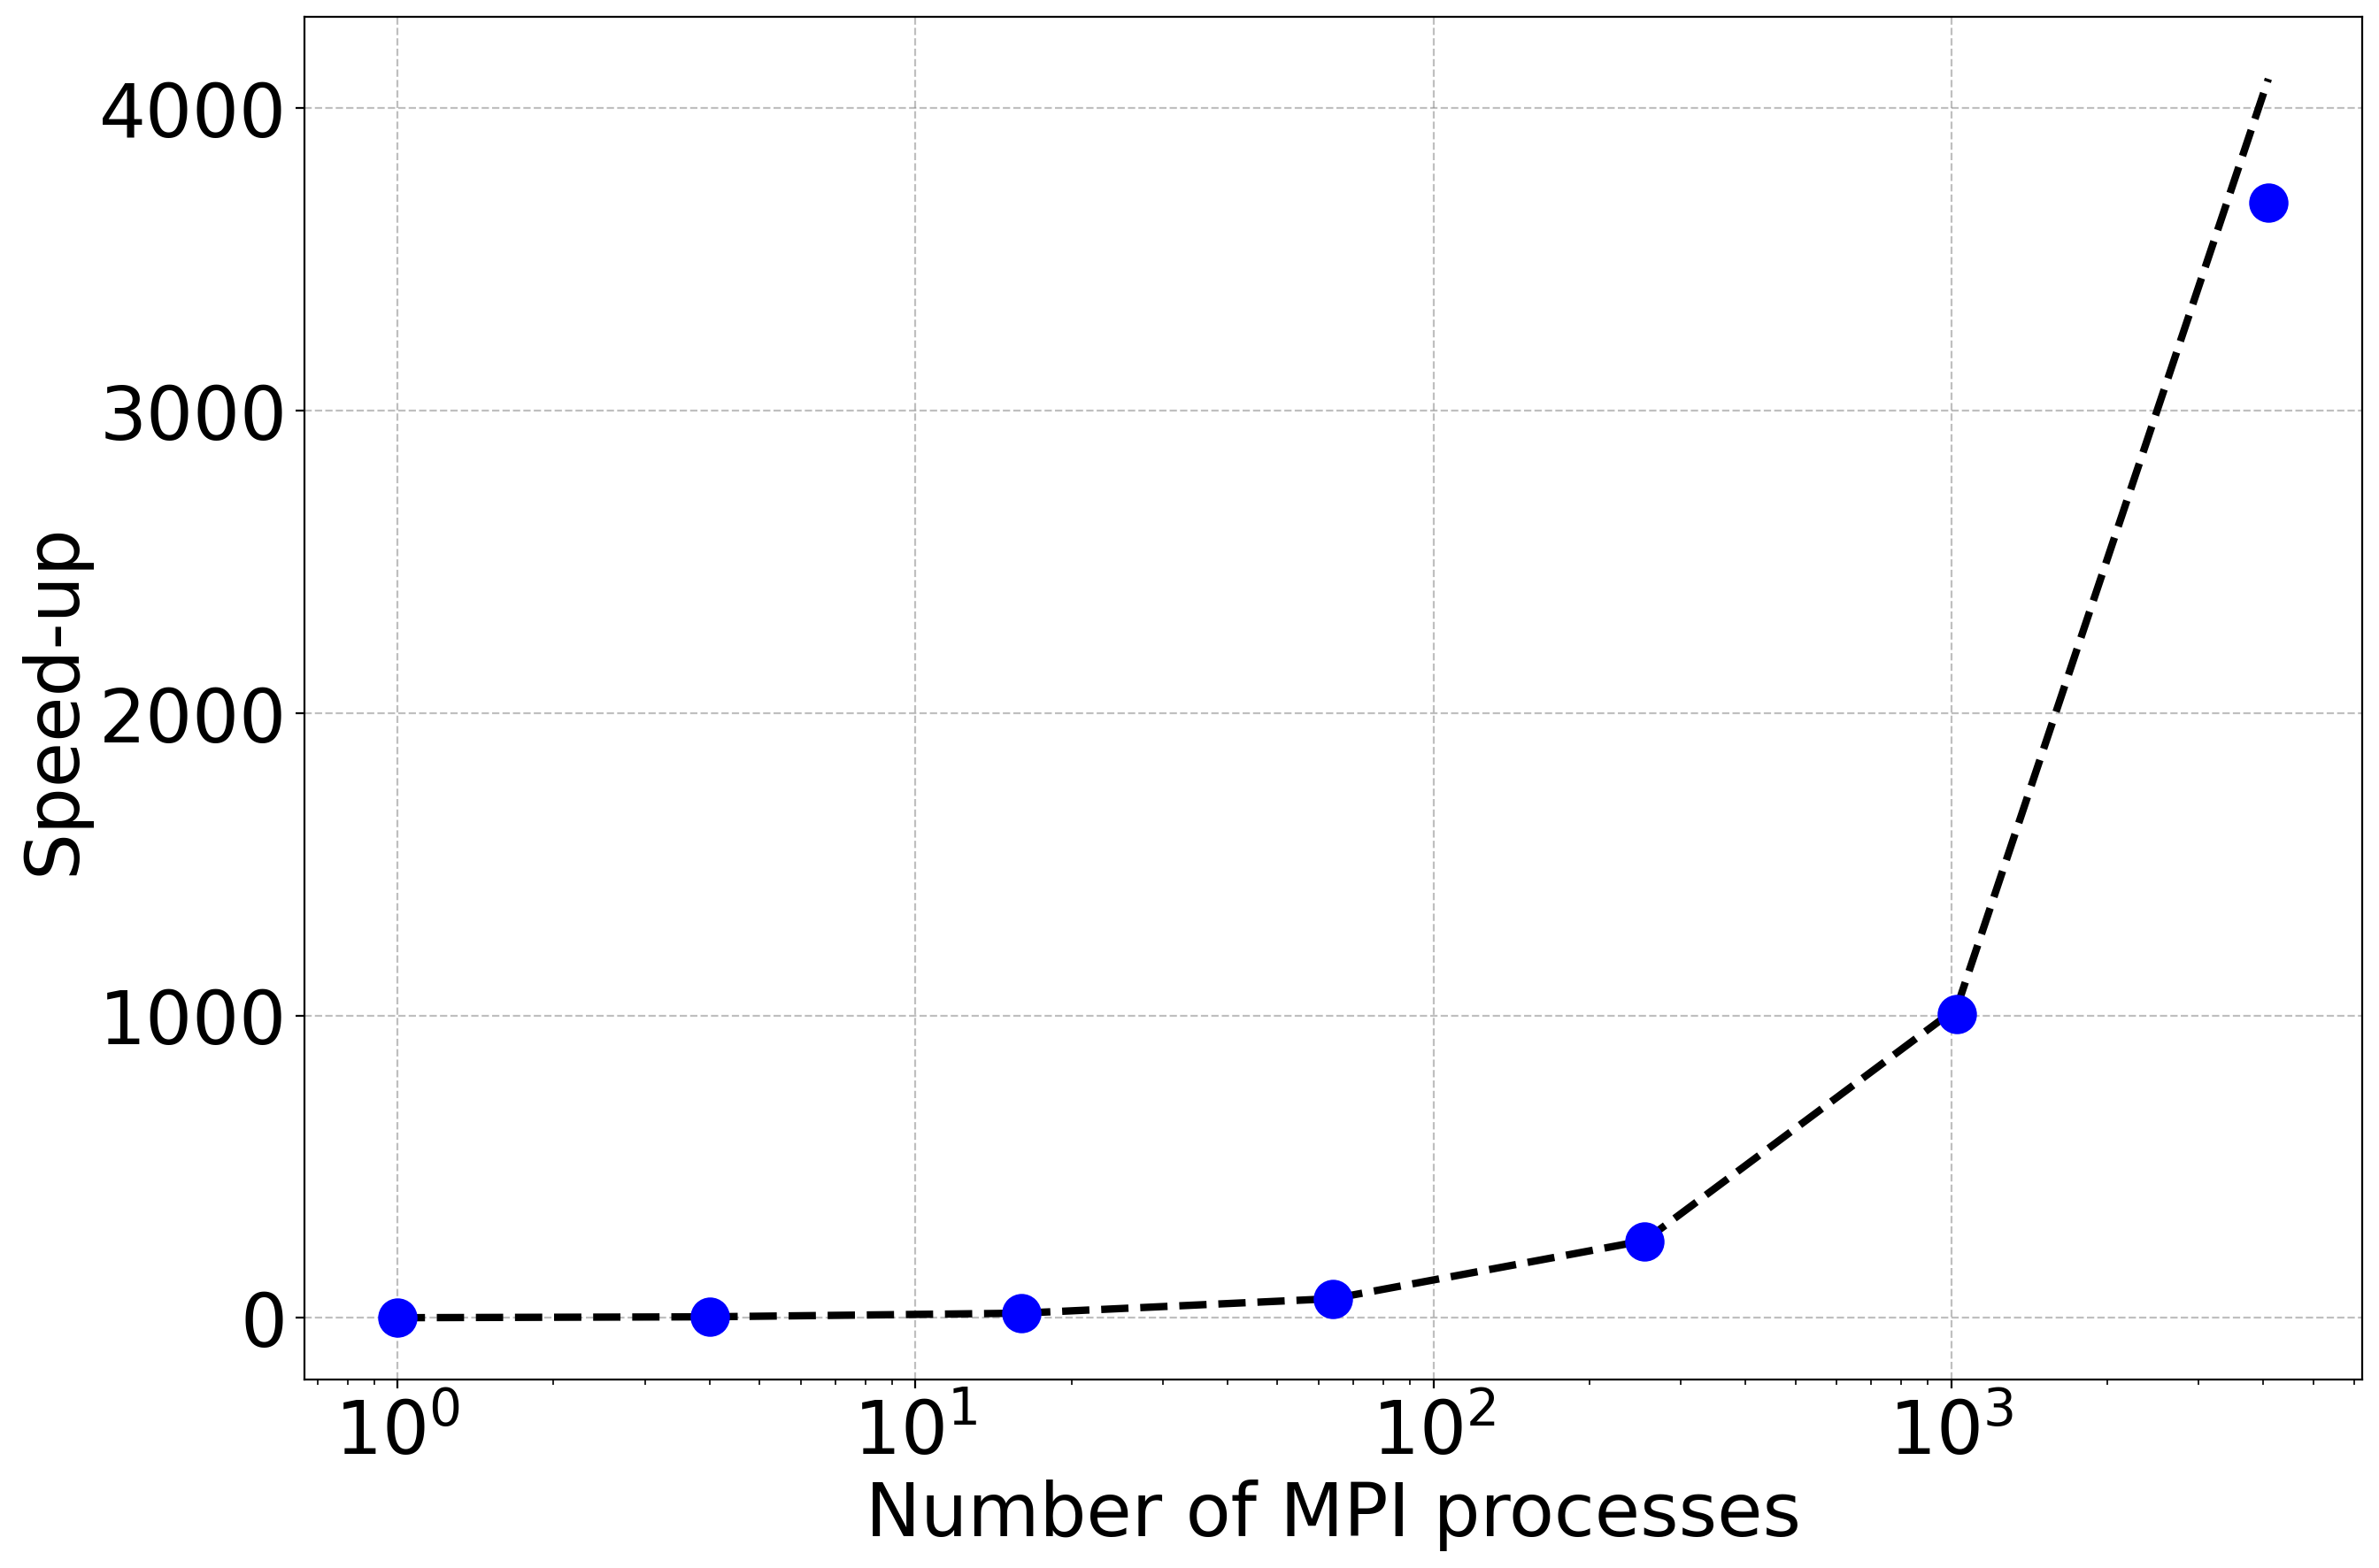
\includegraphics[width=0.75\linewidth]{chapter3_numerical_methods/pictures/speed_up.png}
    \caption{Speed up achieved for distributed parallelism with HYPERION and the migratable task algorithm - ideal speed-up (dashed line) versus actual speed-up (blue dots).
    Data collected for a single immersed body using AMD Rome processors.}
    \label{fig:speed_up}
\end{figure}

%
% [TBB] Ici c'est peut-être le plus délicat.
% On veut pas faire non plus un papier de HPC, donc on peut pas se permettre de rentrer dans tous les détails hyper techniques.
% Mais c'est quand même ECCOMAS, donc il faut pas non plus qu'on ait pas l'air de maîtriser le sujet....
% Je pense qu'on peut découper cette partie en plusieurs sous-parties qui racontent comment on est arrivé au besoin & à l'écriture
% de l'algo avec des tâches migrables
% + Comment ça marche en séquentiel (let's say shared-memory rather than purely sequential, that allows us to immediately include OpenMP considerations), en gros c'est quoi l'algo et comment on relie la taille/longueur/compléxité de la recherche de voisins à l'ordre (en gros cf C&F 2021)
% + Si on utilise une approche classique distribuée où en gros on s'appuie que sur des halos, ça donnerait quoi en terme de taille de halos, en terme de Gb communiqués etc ... -- ça expliquera bien pourquoi il faut faire quelque chose.
% + Notre proposition d'algo distribué basé sur des tâches migrables
%   + Faudra rapidement évoquer la structure de données en liste chaînée pour le traitement contigu des tâches sur un process MPI
%   + On parle de comment la migration se passe : comme les processes ne savent pas forcément s'ils vont recevoir un message, ils doivent attendre indéfiniment
%   + Du coup on a un problème de complétion -- it's quite easy to know if, locally, we still have tasks to accomplish, but it's very hard to know whether another process might send a task ==> we need a consensus algorithm, and there is actually one in the paper by Francez that we can use
% + On oubliera pas de mettre des morceaux de pseudo-code un peu partout pour soutenir notre argumentation -- je ne pense pas qu'il faille prendre le temps d'écrire suffisamment pour que ça soit reproductible par n'importe qui, mais il faut au moins donner suffisamment de détails pour que ça paraisse effectivement faisable
% + Et il va falloir sortir des cas tests aussi à ce moment là ... alors là c'est pas évident non plus parce que la version de l'algo "avec halo" n'existe plus nul part donc il va falloir truander ... à voir !
%

\section{TOWARDS HIGH-FIDELITY SIMULATIONS}\label{sec:high_fidelity}
%
% [TBB] Alors maintenant qu'on a raconté tout ce qu'on a raconté au dessus, il faut absolument mettre l'accent
% sur le fait que ça a rendu possible les simulations 3D à des coûts raisonnables et que sans ces deux optimisations on
% pouvait pas vraiment envisager du 3D massivement parallèle avec IBC.
% Du coup maintenant qu'on a ça, on peut se concentrer sur la LES pour améliorer un peu la fidélité physique d'HYPERION quand
% les maillages ne sont pas DNS-like.
% + On peut mentionner rapidement la légère modification des équations de NS quand on arrive dans le monde de la LES : ajout
% d'une notion de viscosité turbulente à la Boussinesq via un modèle de sous-maille (on a aussi un Prandtl turbulent qui fait
% son apparition du coup)
% + On peut parler des ambitions d'ajout de loi de paroi - on est pas forcé d'avoir des résultats je pense si on mentionne bien
% qu'il s'agit d'un travail de doctorat en cours, mais il faudrait peut-être déjà donner des billes sur comment on pense faire
% et où on aimerait brancher ça.
% + Attention quand même à ce dernier point ... publier des choses comme ça, en avance de phase et sans résultats, ça peut aussi
% conduire à ce qu'une autre équipe y arrive avant nous et le publie - il faut qu'on détermine jusqu'où on avance nos pions.
%

The two algorithms/strategies presented in sections~\ref{sec:rasterization} and~\ref{sec:migratable_tasks} made possible running massively parallel simulations in three dimensions with HYPERION: before the introduction of the former, detecting solid cells on realistic meshes of the order of $10^8$ cells would take several days, and before the introduction of the latter, three-dimensional computations with immersed objects would be too expensive and, most often, would fail altogether during the spiral walks.
In the high Mach and Reynolds numbers regimes where this study places itself, direct numerical simulations (DNS) are out of reach because of their prohibitive computational cost.
However, we aim at running large eddy simulations (LES) with an \emph{ad hoc} subgrid-scale model to improve the predictive capabilities of HYPERION in the compressible regime even on coarse meshes - gaining the ability to run three-dimensional simulations was a first step in that direction.

An in-depth presentation of the LES equations for compressible flows is out of the scope of this paper (the interested reader is referred \emph{e.g.} to Garnier \emph{et al.} \cite{Garnier2009}), but recall that solving the LES equations implies using a filtered version of the compressible Navier-Stokes equations~\eqref{eq:cons_ns}-\eqref{eq:cons_ns_vectors}, among which the momentum equations now read:

\begin{equation}
    \dfrac{\partial \bar\rho \tilde{u}_i}{\partial t} + \dfrac{\partial \bar\rho \tilde{u}_i\tilde{u}_j}{\partial x_j} + \dfrac{\partial \bar p}{\partial x_i} - \dfrac{\partial \overset{\smile}{\sigma}_{ij}}{\partial x_j} = -\dfrac{\partial \tau_{ij}}{\partial x_j} + \dfrac{\partial}{\partial x_j} \left( \overline{\sigma_{ij}} - \overset{\smile}{\sigma}_{ij}\right),
    \label{eq:les_momentum_eqns}
\end{equation}

where the $\tilde{\cdot}$ overset denotes Favre averaging, the $\bar\cdot$ overset denotes Reynolds averaging, and $\overset{\smile}{\sigma}_{ij}$ depends on the computable rate-of-strain tensor:

\begin{equation}
    \overset{\smile}{\sigma}_{ij} = \mu(\tilde{T}) \left( 2 \tilde{S}_{ij} - \dfrac{2}{3}\delta_{ij}\tilde{S}_{kk} \right),~~ \tilde{S}_{ij} = \dfrac{1}{2}\left( \dfrac{\partial\tilde{u}_i}{\partial x_j} + \dfrac{\partial \tilde{u}_j}{\partial x_i}\right).
    \label{eq:sigma_smile}
\end{equation}

All overset variables are computable whereas we need a closure for the subgrid-scale stress tensor $\tau_{ij}$.
In HYPERION, we follow a Boussinesq type hypothesis \cite{boussinesq1877essai} that leads to the subgrid-scale stress tensor having the following mathematical form:

\begin{equation}
    \tau_{ij} - \dfrac{1}{3}\delta_{ij}\tau_{kk} = - 2 \bar\rho \nu_{\text{sgs}} \left( \tilde{S}_{ij} - \dfrac{1}{3} \delta_{ij}\tilde{S}_{kk} \right),
    \label{eq:boussinesq_les}
\end{equation}

where $\nu_{\text{sgs}}$ represents a scalar subgrid viscosity that is left to be modelled.
In the present study we rely on the Wall-Adapting Local Eddy-viscosity model (WALE) by Ducros \emph{et al.} \cite{ducros1998wall} to run preliminary tests with the LES version of HYPERION.

\subsection{Taylor-Green Vortex}\label{ssec:test_tgv}

Before trying to evaluate the quality of the LES computations in the presence of immersed obstacles, let us run a very classical viscous test case that will allow us to check the implementation of the WALE model.

We are therefore considering the case of a Taylor-Green vortex which set-up and reference solution can be obtained from the 3$^{\text{rd}}$ international workshop on higher-order CFD methods \cite{diosady2015case}.
The domain is a periodic cube of dimensions $[-\pi, \pi]^3$, and the initial solution is given by the following expressions:

\begin{equation}
    \left\lbrace
    \begin{array}{ccl}
        u &=& \sin{\left( x \right)} \cos{ \left( y \right) } \cos{ \left( z \right) }, \\[0.6em]
        v &=& -\cos{\left( x \right)} \sin{ \left( y \right) } \cos{ \left( z \right) }, \\[0.6em]
        w &=& 0, \\[0.6em]
        p &=& \dfrac{1}{\gamma M_{\infty}^2} + \dfrac{1}{16}\left( \cos(2 x) + \cos(2 y) \right) \left( \cos(2 z) + 2\right), \\[0.6em]
        \rho &=& \gamma M_{\infty}^2 p.
    \end{array}
    \right.
\end{equation}

In this problem, we do not intend to validate in any way the behavior of the immersed boundaries algorithms.
Rather, we shall inspect the temporal evolution of the kinetic energy $E_k$ and of the enstrophy $\varepsilon$ integrated over the domain and compare it to the reference solution \cite{diosady2015case}.
Note that the mathematical expression used in this study for the kinetic energy is:

\begin{equation}
    E_k = \dfrac{1}{N^3} \sum_{i,j,k} \dfrac{1}{2} \rho_{i,j,k} \left(u_{i,j,k}^2 + v_{i,j,k}^2 + w_{i,j,k}^2\right),
    \label{eq:kinetic_eqn}
\end{equation}

and that of the enstrophy is:

\begin{equation}
    \epsilon = \dfrac{1}{N^3}\sum_{i,j,k} \dfrac{1}{2} \rho_{i,j,k} \left( \omega_{x; i,j,k}^2 + \omega_{y; i,j,k}^2 + \omega_{z; i,j,k}^2 \right),
    \label{eq:enstrophy}
\end{equation}

where $N$ stands for the number of cells along one side of the domain (assuming the Cartesian mesh is homogeneous), and $\mathbf{\omega} = \nabla \times \mathbf{u}$ is the vorticity.
To observe the convergence of the solution towards the reference solution, computations results on meshes of sizes $64^3$ and $512^3$ are shown here.
The computations were furthermore run using the AUSM$^+$-up Riemann solver in conjunction with the fifth-order TENO reconstruction scheme.

\begin{figure}[ht!]
    \centering
    \begin{tabular}{cc}
        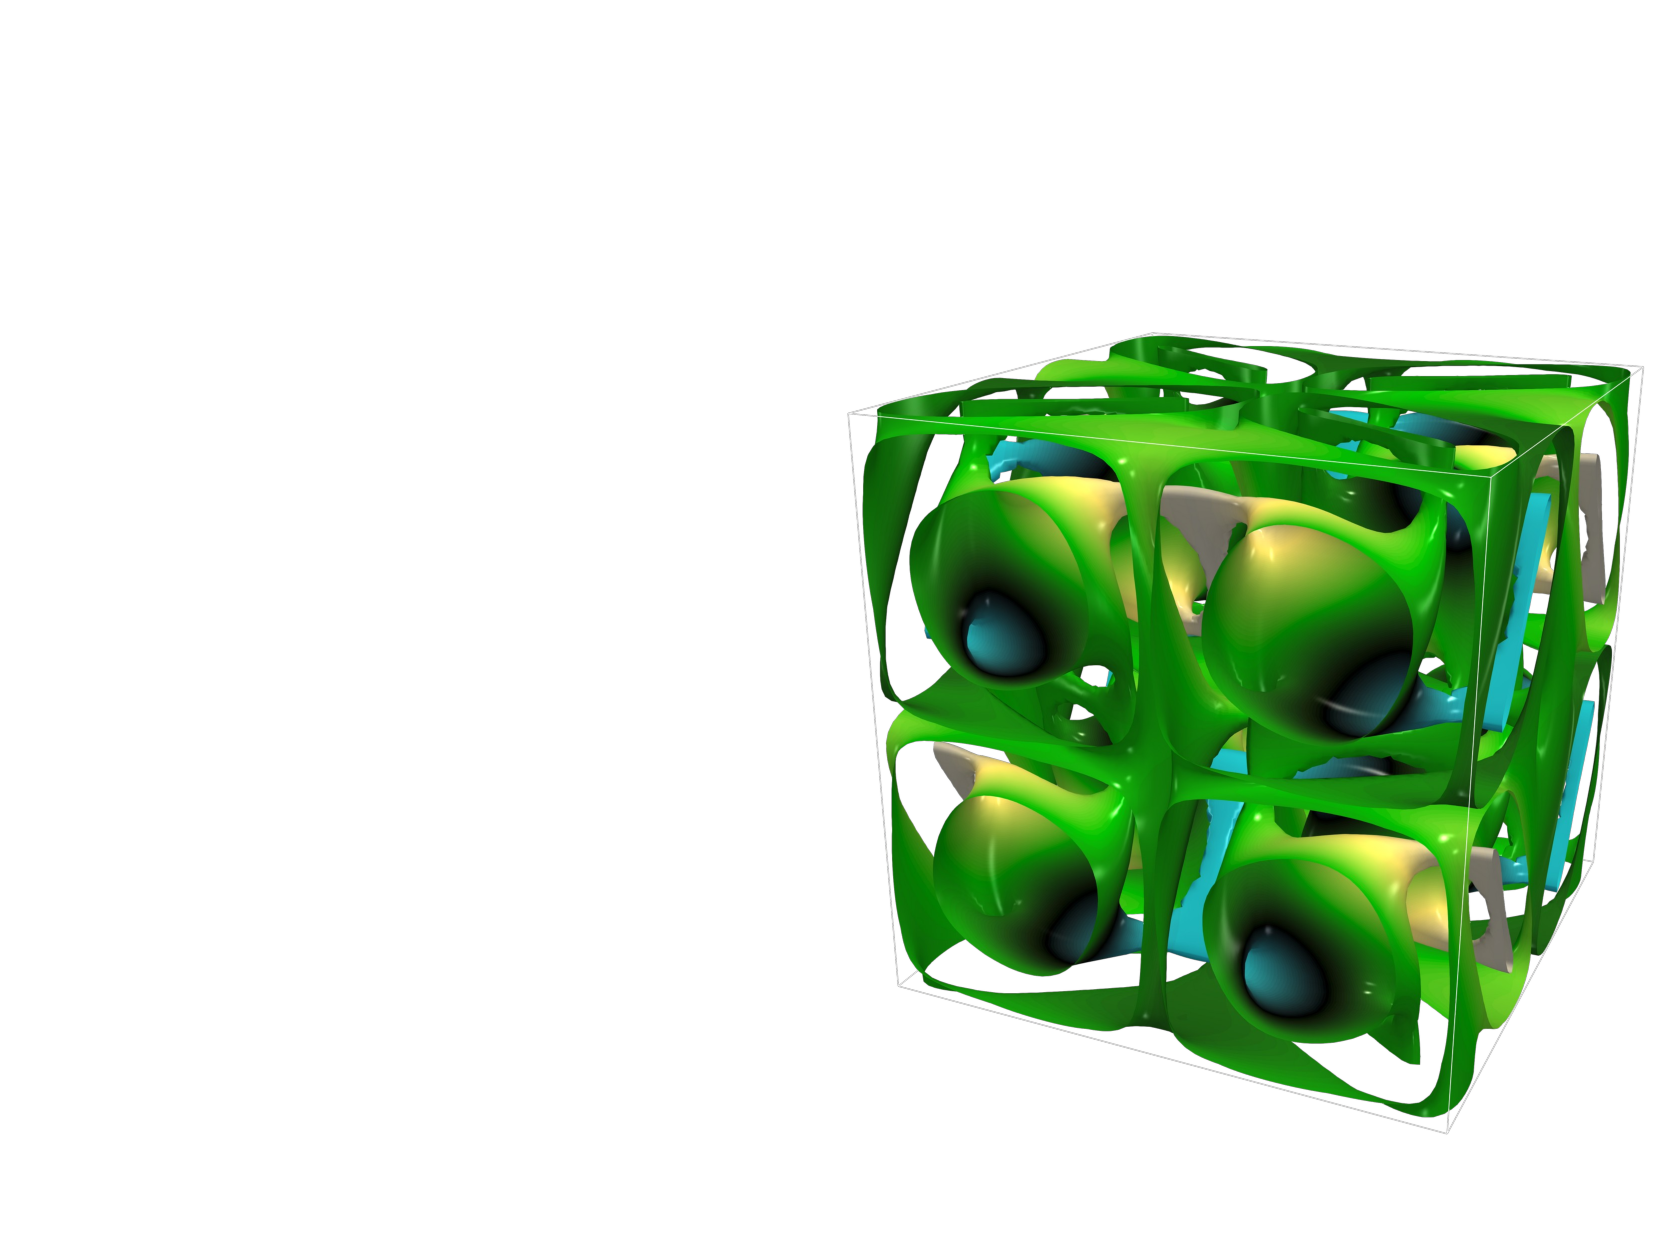
\includegraphics[width=0.45\linewidth]{chapter3_numerical_methods/pictures/TGV_coarse.pdf} &
        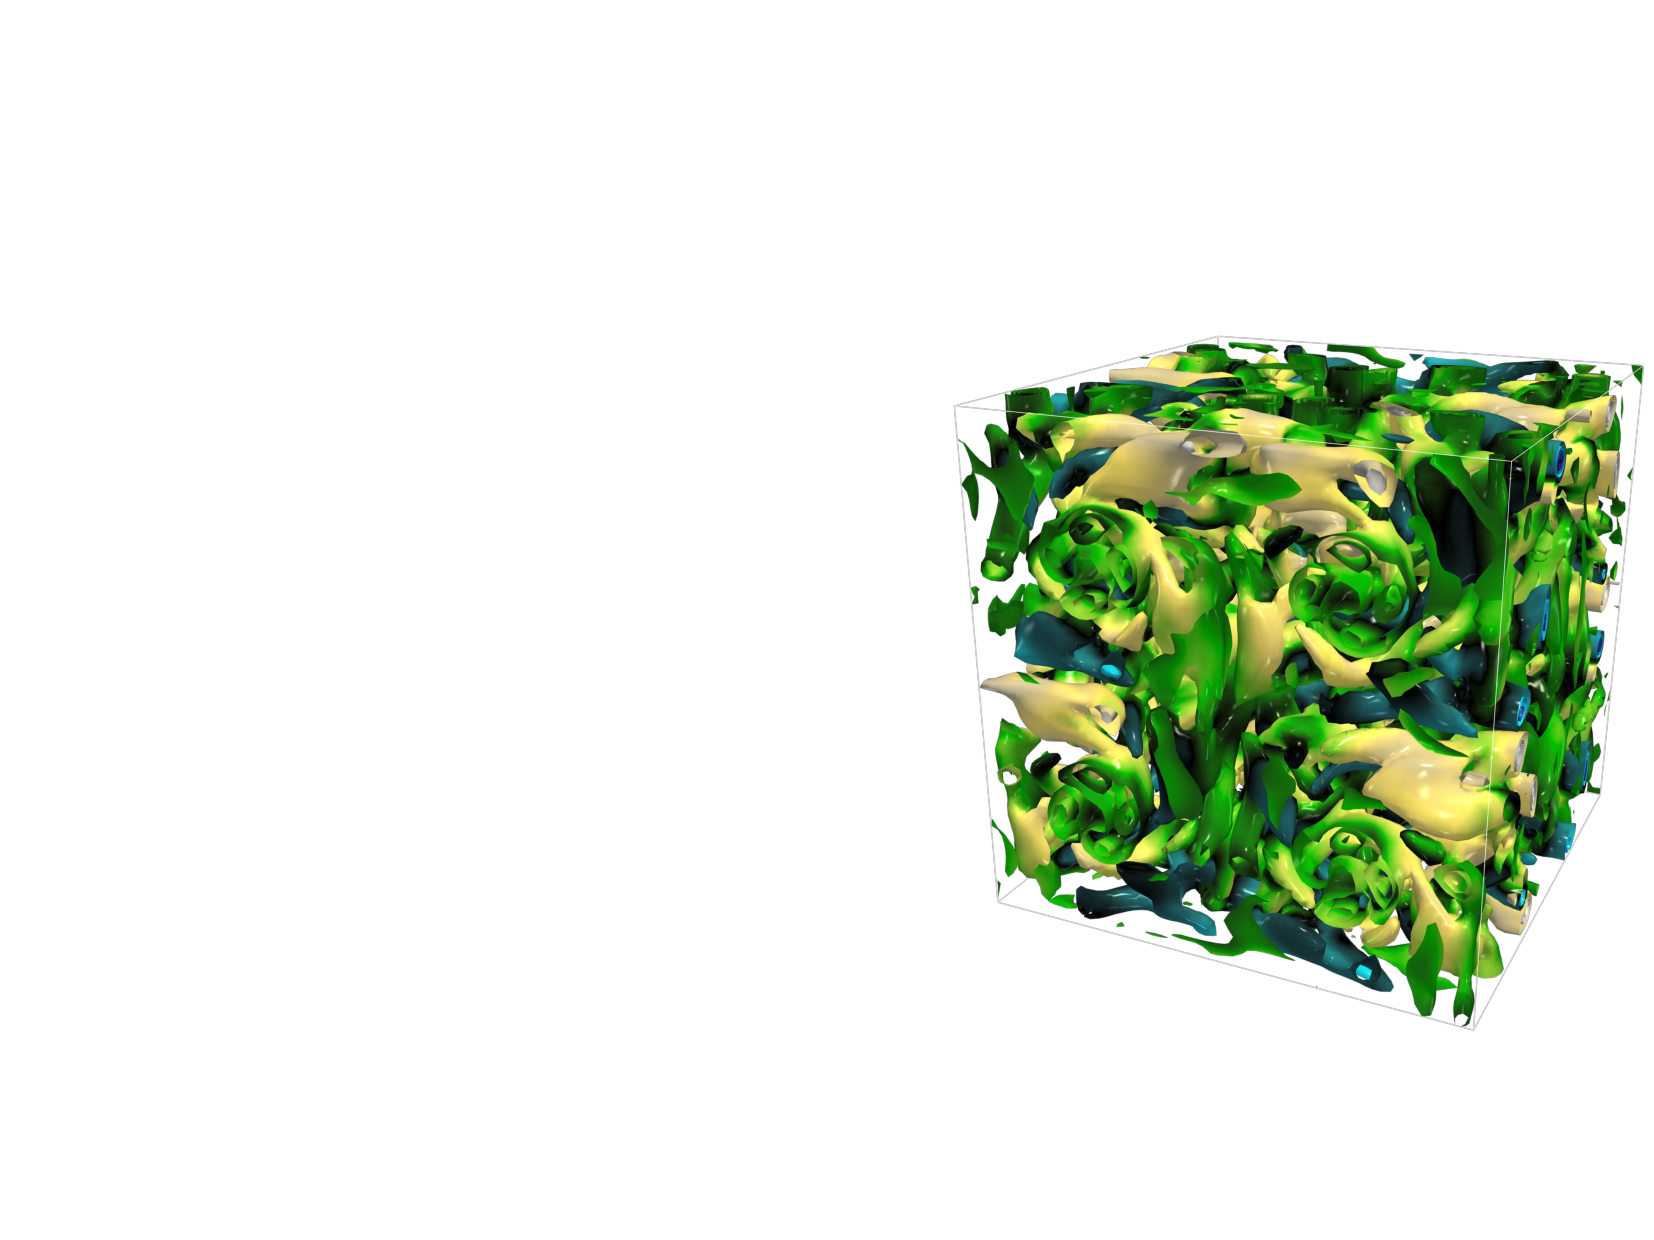
\includegraphics[width=0.45\linewidth]{chapter3_numerical_methods/pictures/TGV_fine.pdf} \\
        (a) & (b)
    \end{tabular}
    % \caption{Snapshot of the state of the Taylor-Green vortex after $20$ characteristic times, (a) on the $64^3$ mesh and (b) on the $512^3$ mesh.
    % Isocontours of the Q-criterion are represented, colored by the norm of the vorticity.}
    \caption{Snapshots of the state of the Taylor-Green vortex after (a) $1$ characteristic time and (b) $20$ characteristic times on the $64^3$ mesh.
    Isocontours of enstrophy are represented, colored by the magnitude of velocity.}
    \label{fig:TGV_view}
\end{figure}

Figure~\ref{fig:TGV_view} presents the three-dimensional structures present in both the coarse and the fine flow as isocontours of the Q-criterion colored by the magnitude of the vorticity.
As expected, the turbulence is allowed to develop itself down to much smaller scales on the fine mesh.

\begin{figure}[ht!]
    \centering
    \begin{tabular}{cc}
        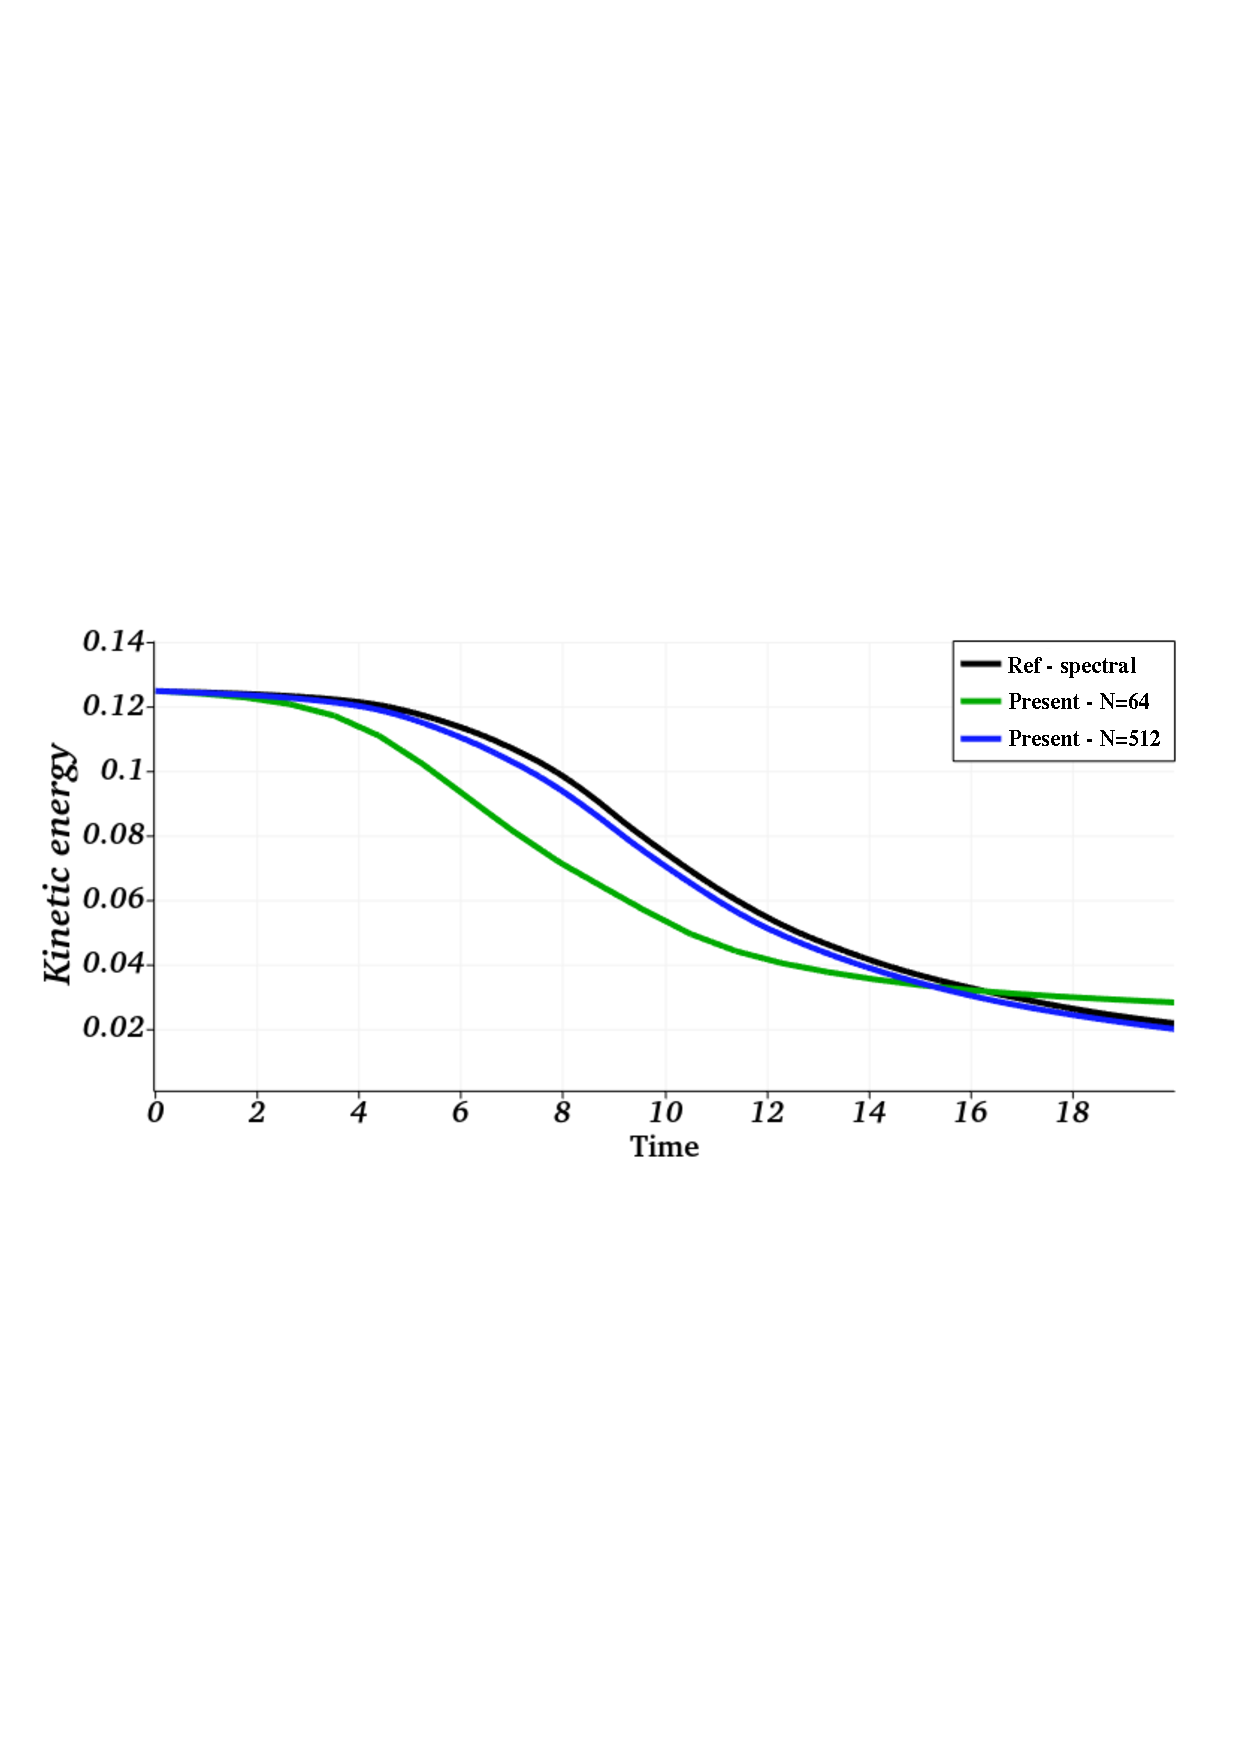
\includegraphics[width=0.47\linewidth]{chapter3_numerical_methods/pictures/TGV_energy_v2.pdf} &
        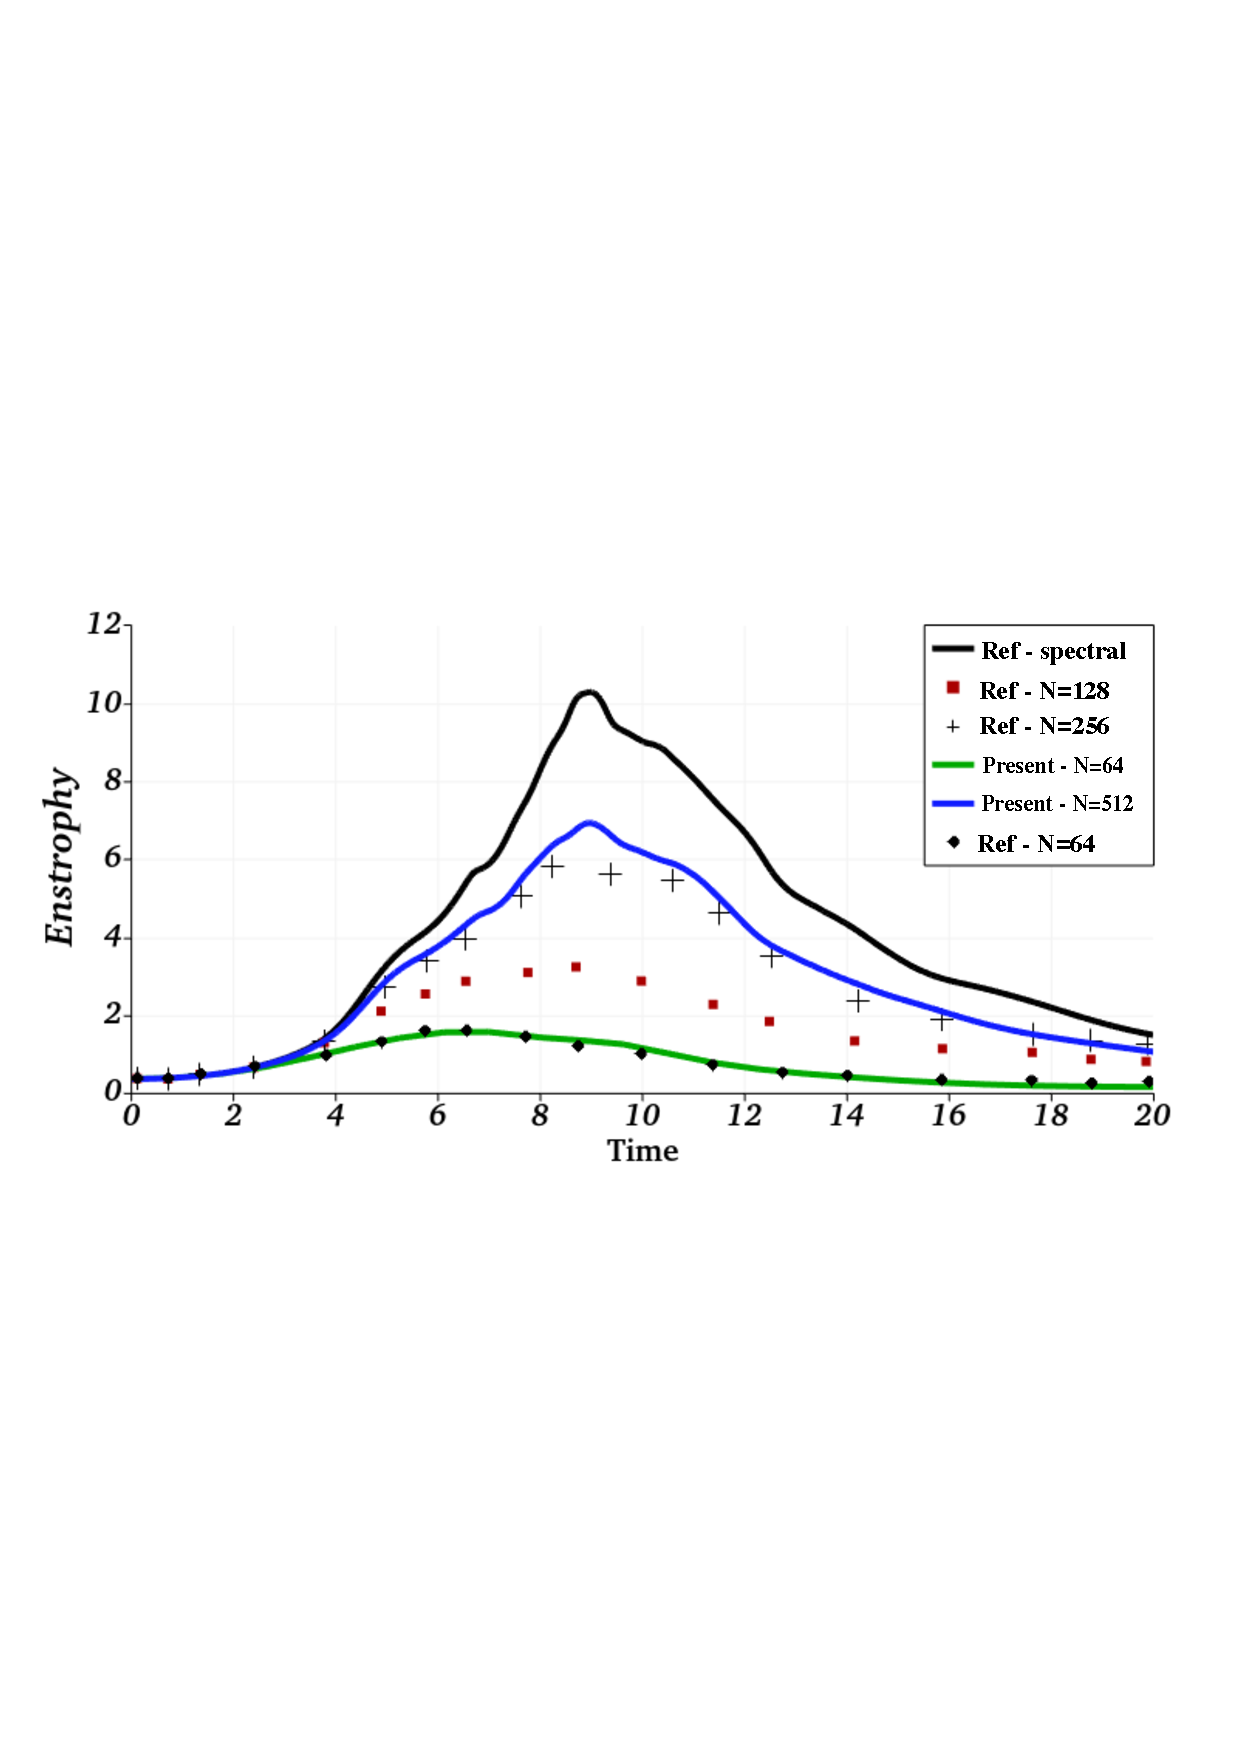
\includegraphics[width=0.47\linewidth]{chapter3_numerical_methods/pictures/TGV_enstrophy_v2.pdf} \\
        (a) & (b)
    \end{tabular}
    \caption{Comparison of the temporal evolution of (a) the kinetic energy (see equation~\eqref{eq:kinetic_eqn}) and (b) the enstrophy (see equation~\eqref{eq:enstrophy}) against the $512^3$ spectral computation from \cite{diosady2015case} (black line) and the high-order computations from \cite{giangaspero2015case} (symbols).}
    \label{fig:TGV_comparison}
\end{figure}

Figure~\ref{fig:TGV_comparison} introduces a more quantitative comparison between the present results and both the reference spectral computation conducted on a $512^3$ mesh in \cite{diosady2015case} and some high-order reference computations from \cite{giangaspero2015case}.
The results are satisfactory and show the convergence towards the reference for both metrics - the kinetic energy, figure~\ref{fig:TGV_comparison}(a) and the enstrophy, figure~\ref{fig:TGV_comparison}(b).
The results in terms of enstrophy seem further away but in another exhaustive study (unpublished yet) the authors show the prime importance of the approximate Riemann solver on the quality of the enstrophy production in a finite-volume code, and although the AUSM$^+$-up solver is particularly adapted at handling all-speed flows with hypersonic regions, it might not be the ideal solver for fine turbulence behavior - such a discussion is however out of the scope of this paper.

\subsection{Double cone}\label{ssec:test_double_cone}

With the implementation of the subgrid-scale model validated by the turbulence testcase discussed in paragraph~\ref{ssec:test_tgv}, we move on to the study of the flow around two documented configurations in supersonic or hypersonic regimes.

\begin{figure}[ht!]
    \centering
    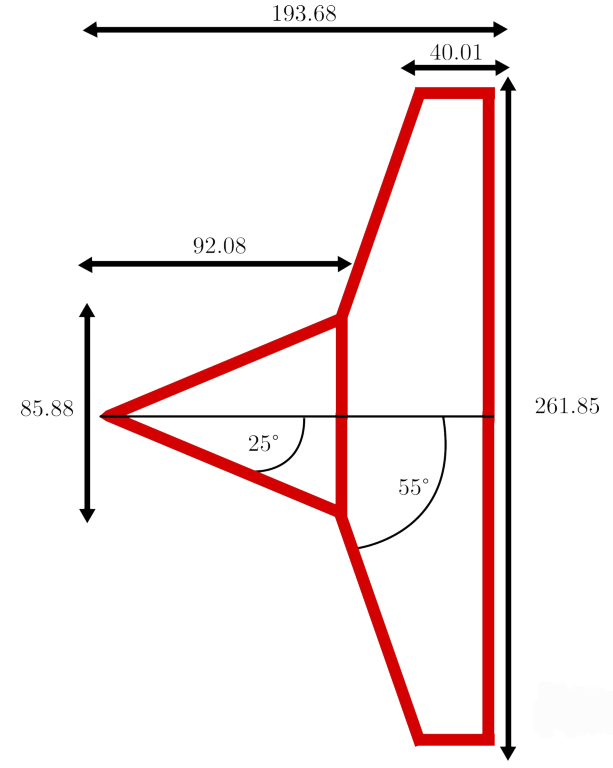
\includegraphics[width=0.40\linewidth]{chapter3_numerical_methods/pictures/double_cone.pdf}
    \caption{Geometrical details of the double-cone configuration.}
    \label{fig:double_cone_geom}
\end{figure}

For the first immersed boundary condition testcase, the hypersonic flow over an axisymmetric double cone configuration (see figure~\ref{fig:double_cone_geom}) is studied at Mach number $12.2$ and Reynolds number $14 \times 10^6$.
The wall temperature is fixed at $1.75T_{\infty}$.
The results presented below correspond to meshes made of $1,200,000$ and $4,000,000$ cells, qualified of coarse and fine, respectively (as it is an axisymmetric obstacle, the simulation itself has been treated as a two-dimensional, axisymmetric simulation).

A qualitative visualization of the resulting flow is provided on figure~\ref{fig:double_cone_schlieren} in the form of a numerical Schlieren image.
It mostly shows the regions where strong changes in density occur, allowing the user to visualize the shock and contact waves, and, like in the present case, the boundary layer developing along the wall.
An inset has been added to the figure to put the light on the lambda-shock pattern found after the boundary layer passes the recirculation region and reattaches itself to the wall of the second cone.

\begin{figure}[ht!]
    \centering
    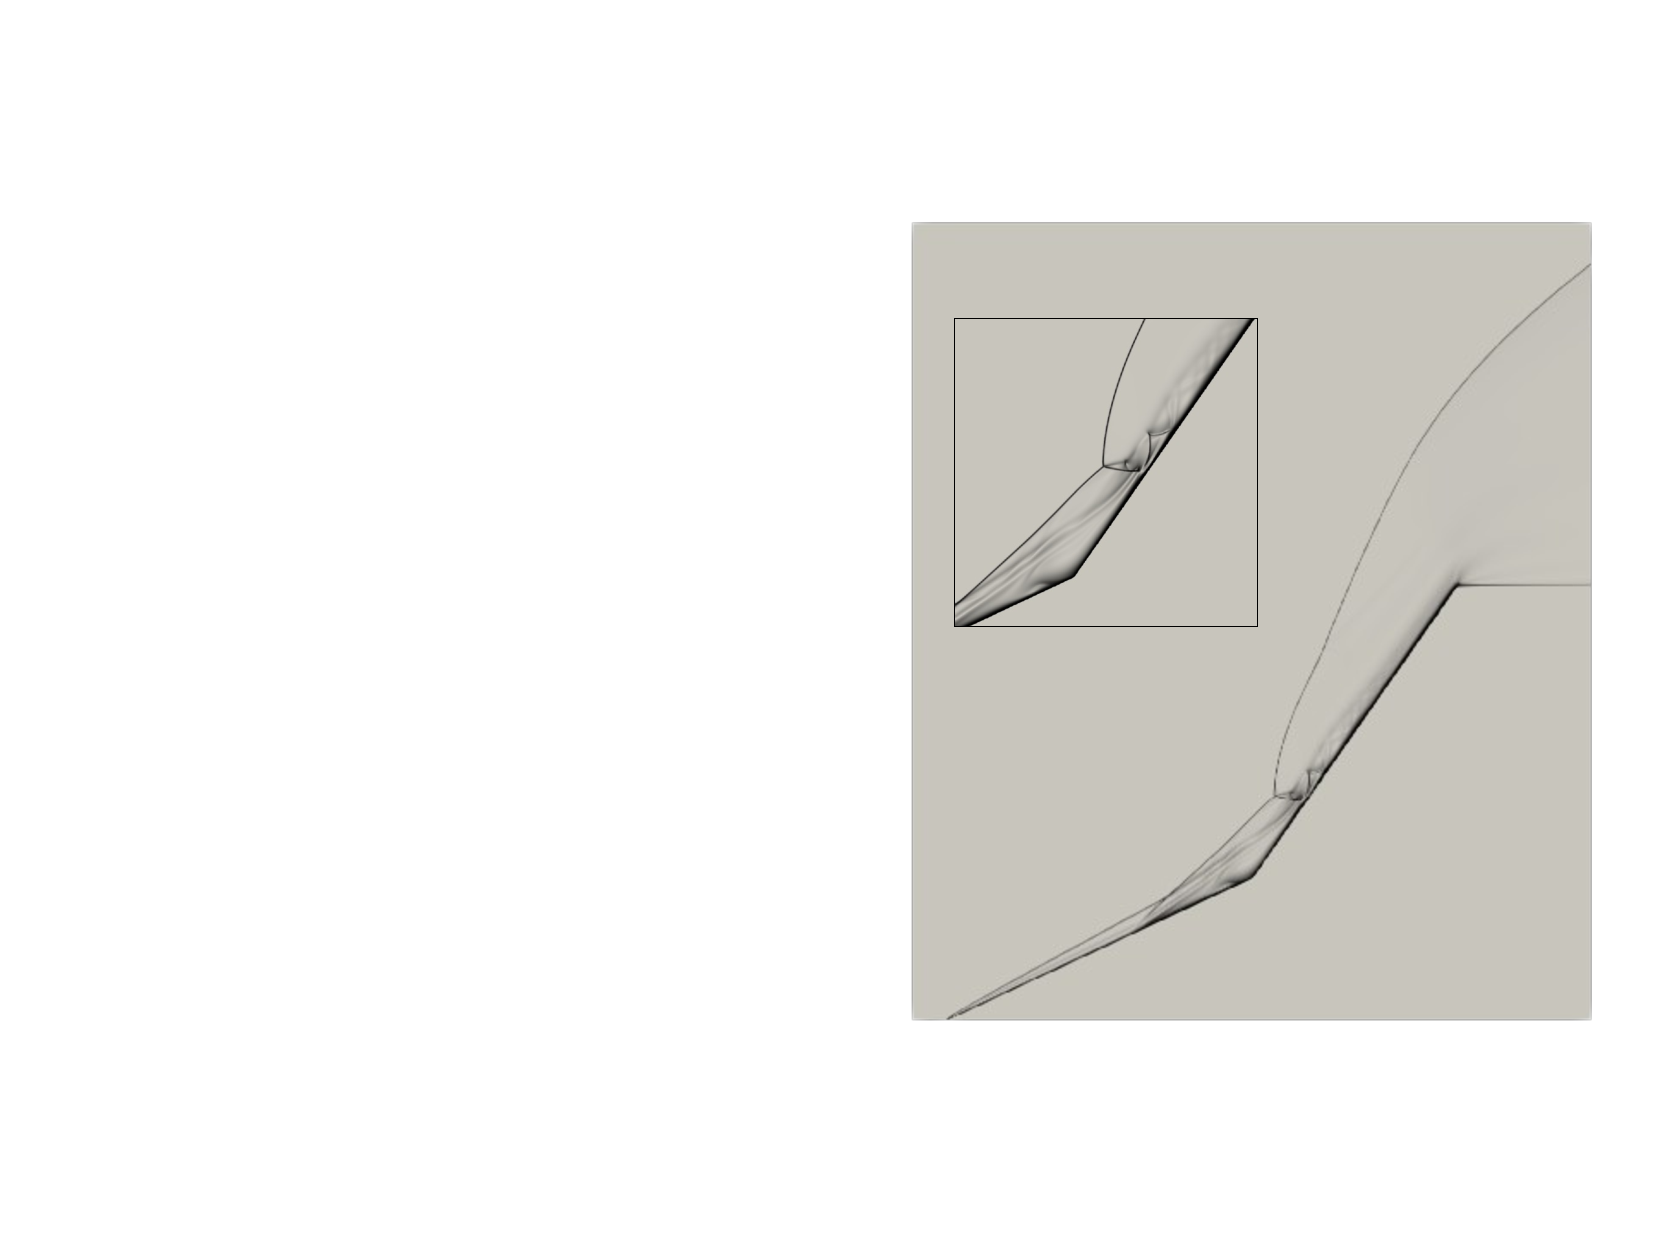
\includegraphics[width=0.35\linewidth]{chapter3_numerical_methods/pictures/double_cone_schlieren.pdf}
    \caption{Numerical Schlieren imaging of the flow around the double cone configuration.
    The inset zooms in on the lambda-shock pattern found after the recirculation region at the change of wall angle.}
    \label{fig:double_cone_schlieren}
\end{figure}

In a more quantitative manner, the wall pressure and the wall heat flux are compared against the experimental results obtained by MacLean \emph{et al.} \cite{MacLean2014} - see figure~\ref{fig:double_cone_comp}(a) and (b).
Without much effort, the wall pressure is correctly predicted - figure~\ref{fig:double_cone_comp}(a) - because it is mostly driven by the inviscid behavior of the simulation and does not depend too much on the resolution of the near-wall flow.
In contrast, the viscous heat flux is not as well predicted because boundary layers are not resolved properly with the immersed boundary method implemented in HYPERION.
Even with a fine mesh, although the peak of heat flux is correctly captured both in terms of coordinates and magnitude, the heat flux levels after the reattachment of the boundary layer are markedly underestimated.
This is a well known shortcoming of any immersed boundary method, and a future study will be dedicated to correcting it with the help of \emph{ad hoc} wall laws.

\begin{figure}[ht!]
    \centering
    \begin{tabular}{cc}
        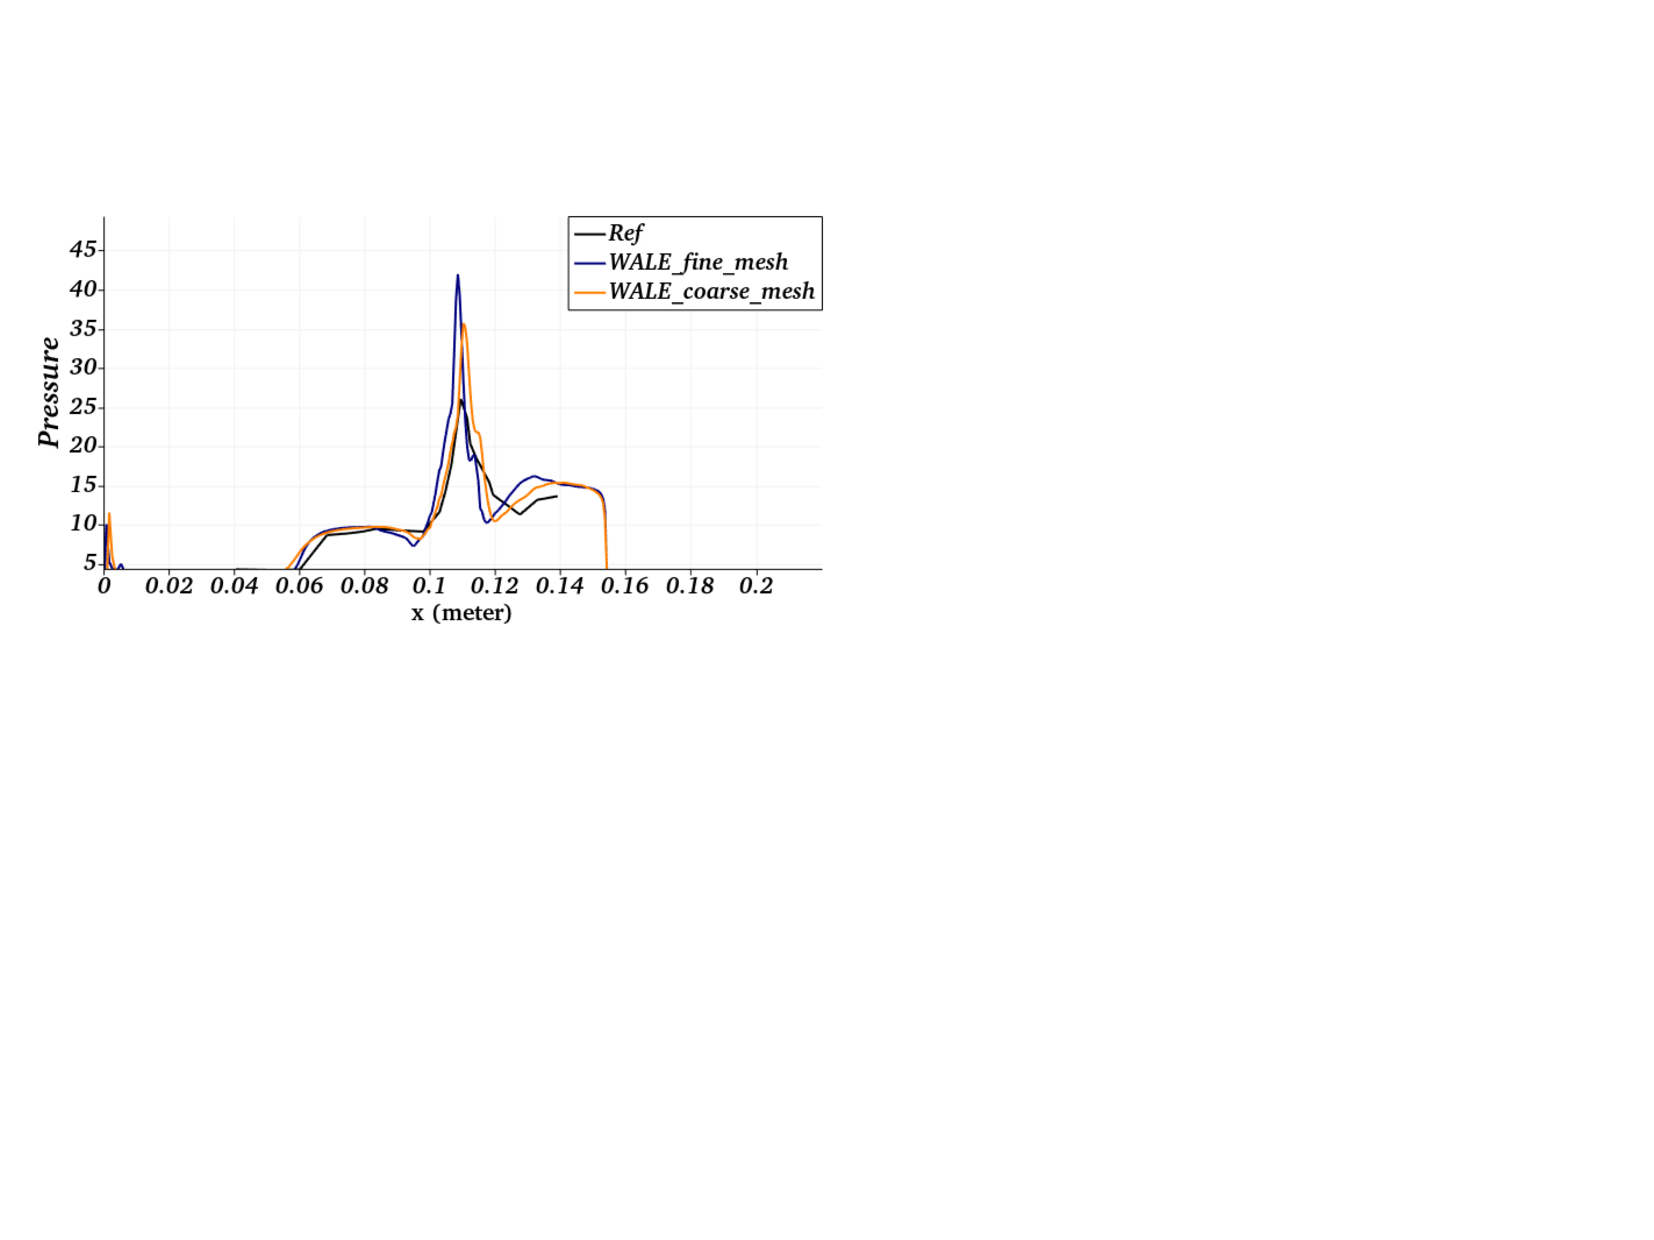
\includegraphics[width=0.47\linewidth]{chapter3_numerical_methods/pictures/double_cone_pressure.pdf} &
        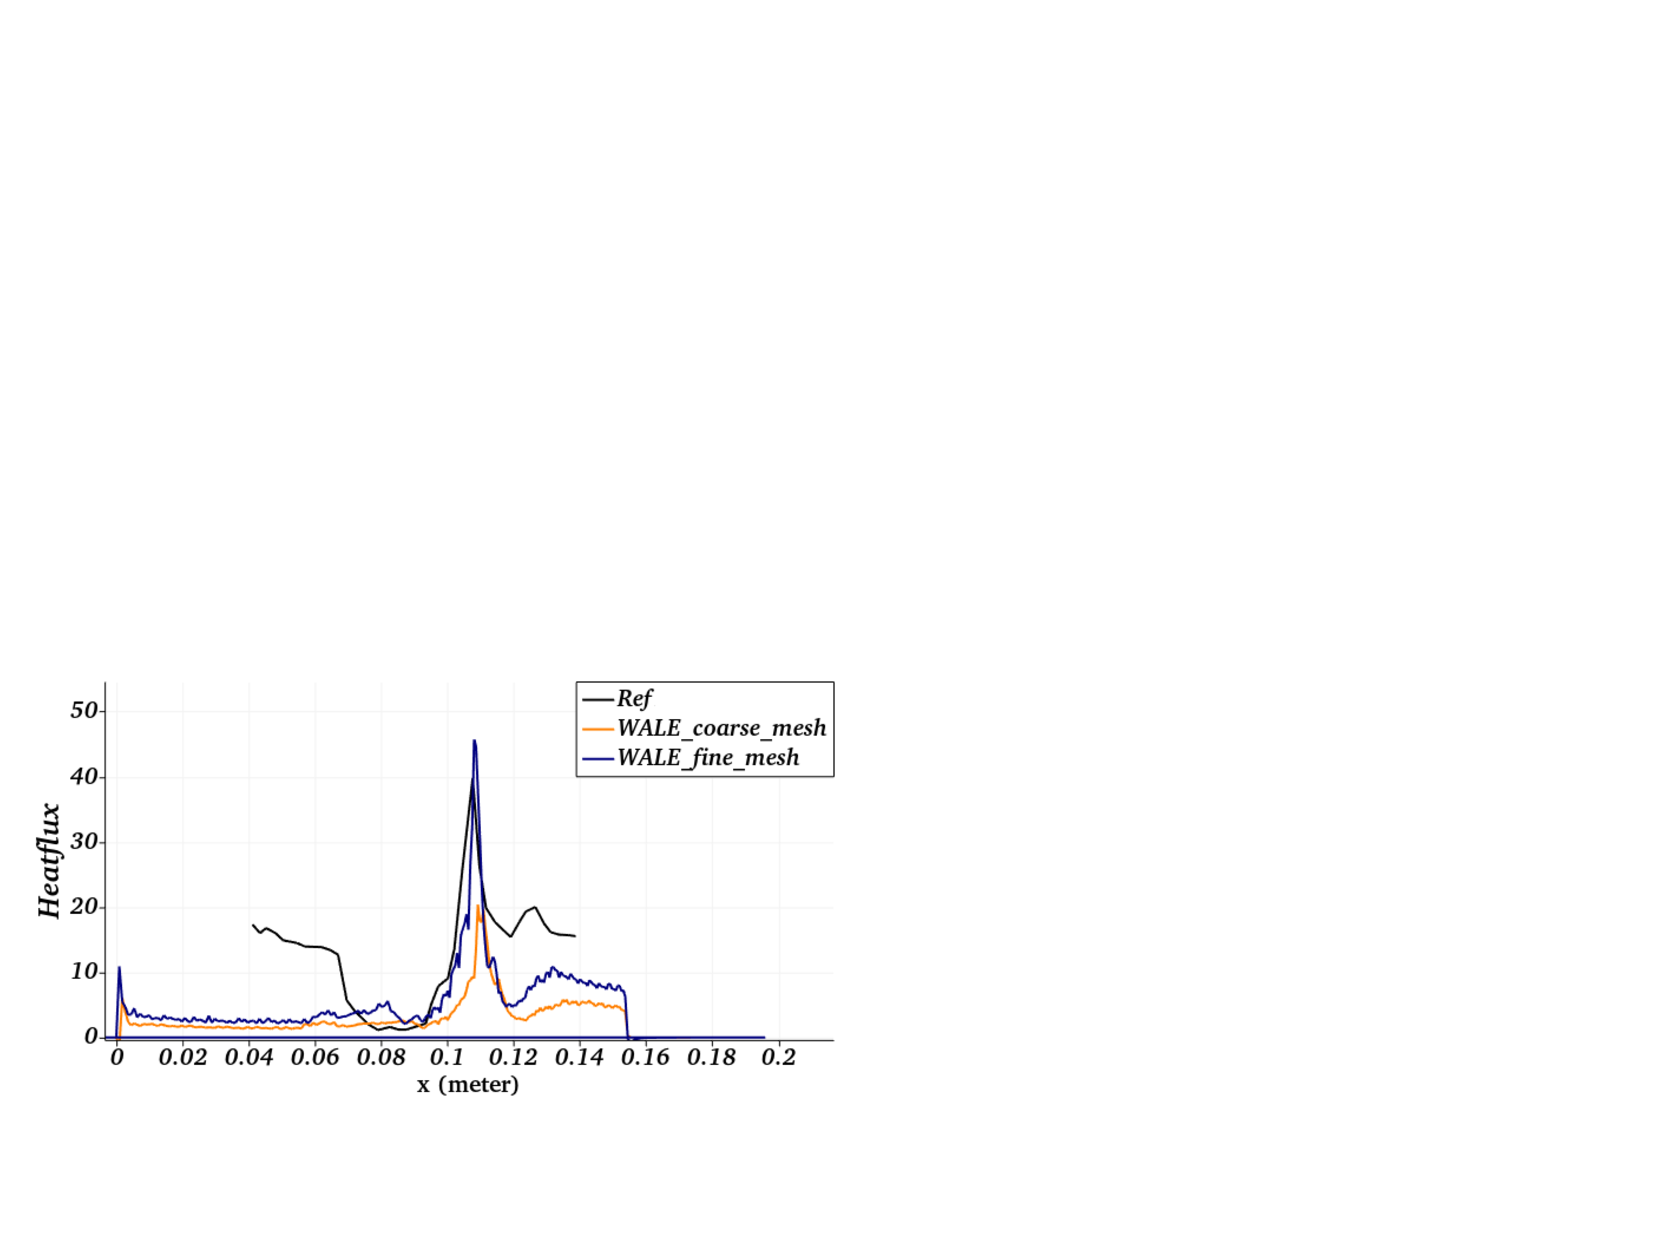
\includegraphics[width=0.47\linewidth]{chapter3_numerical_methods/pictures/double_cone_heat_flux.pdf} \\
        (a) & (b)
    \end{tabular}
    \caption{(a) Pressure coefficient and (b) heat flux obtained at the wall of the double cone.
    Comparison between the results obtained presently on the coarse and fine meshes (orange and blue line, respectively) and the reference solution from MacLean \emph{et al.} \cite{MacLean2014} (black line).}
    \label{fig:double_cone_comp}
\end{figure}


\subsection{Flow study around a double ellipsoid configuration}\label{ssec:test_ellipsoid}

The second immersed boundary condition testcase is the fully three-dimensional flow around a double ellipsoid shape \cite{Aymer1991} described mathematically by the following equations (see figure~\ref{fig:ellipse_geom}):

\begin{equation}
    \left\lbrace
    \begin{aligned}
        &x \leq 0,            &&\left( \frac{x}{0.06} \right)^2 + \left(\frac{y}{0.025} \right)^2 + \left( \frac{z}{0.015} \right)^2 &&= 1 \\
        &x \leq 0,\; z\geq 0, &&\left( \frac{x}{0.035} \right)^2 + \left(\frac{y}{0.0175} \right)^2 + \left( \frac{z}{0.025} \right)^2 &&= 1 \\
        &0 \leq x \leq 0.016, &&\left( \frac{y}{0.025} \right)^2 + \left( \frac{z}{0.015} \right)^2 &&= 1 \\
        &z \geq 0,            &&\left(\frac{y}{0.0175} \right)^2 + \left( \frac{z}{0.025} \right)^2 &&= 1
    \end{aligned}
    \right.
    \label{eq:double_ellipsoid_eqns}
\end{equation}

\begin{figure}[ht!]
    \centering
    \begin{tabular}{cc}
        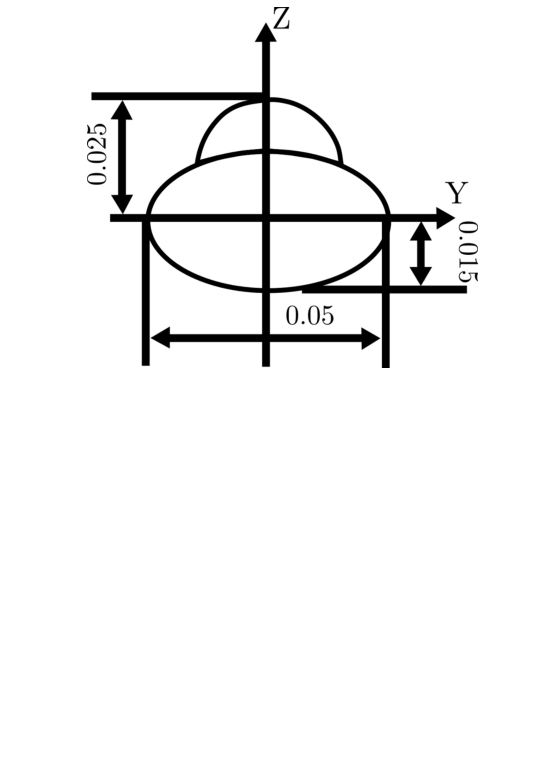
\includegraphics[width=0.35\linewidth]{chapter3_numerical_methods/pictures/ellipse_part1.pdf} &
        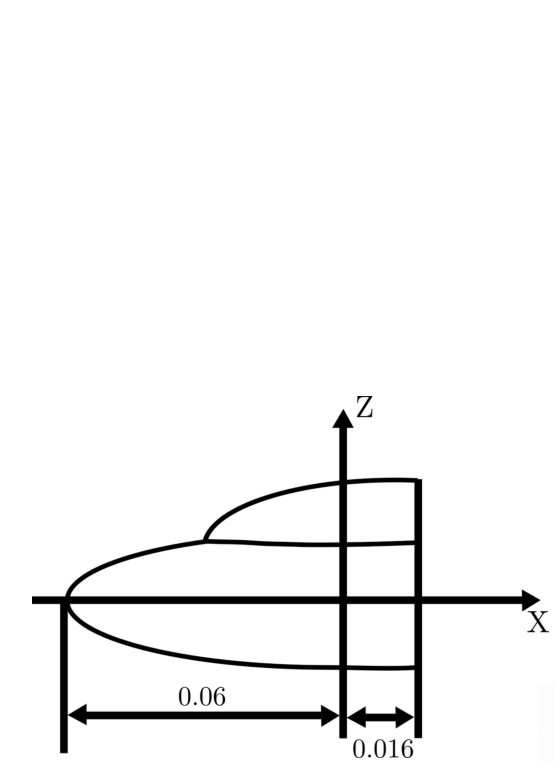
\includegraphics[width=0.45\linewidth]{chapter3_numerical_methods/pictures/ellipse_part2.pdf}
    \end{tabular}
    \caption{Geometrical details of the double ellipsoid configuration.}
    \label{fig:ellipse_geom}
\end{figure}

For that flow, the Mach number is set at $8.15$, the Reynolds number is set at $16.7\times 10^6$ and the freestream angle of attack is set at $30^{\circ}$.
The Cartesian mesh contains approximately $7\times 10^7$ cells, and the double ellipsoid object is tesselated using approximately $2\times 10^5$ triangles; the computation was conducted on $4096$ AMD Rome processors, using $2048$ MPI processes and $2$ OpenMP threads per process, and lasted approximately $48$ hours before the wall quantities could be said to be converged (see below).
Note that this computation, both in terms of manipulation of the immersed object and in terms of computational performance, is made possible only thanks to the two algorithms presented above in sections~\ref{sec:rasterization} and~\ref{sec:migratable_tasks} respectively - without massive parallelism, the time-to-results for this computation would have been unrealistic.

A first quantitative visualization of the flow is given in figure~\ref{fig:ellipse_3D}, where both numerical Schlieren imaging and three-dimensional isocontours of the Q-criterion are presented.
The strong shock waves can be clearly seen around the object whereas the wake seems characterized by multiple contact waves and large-scale turbulent structures that the LES simulation is able to capture, as expected.

\begin{figure}[ht!]
    \centering
    % \begin{tabular}{cc}
        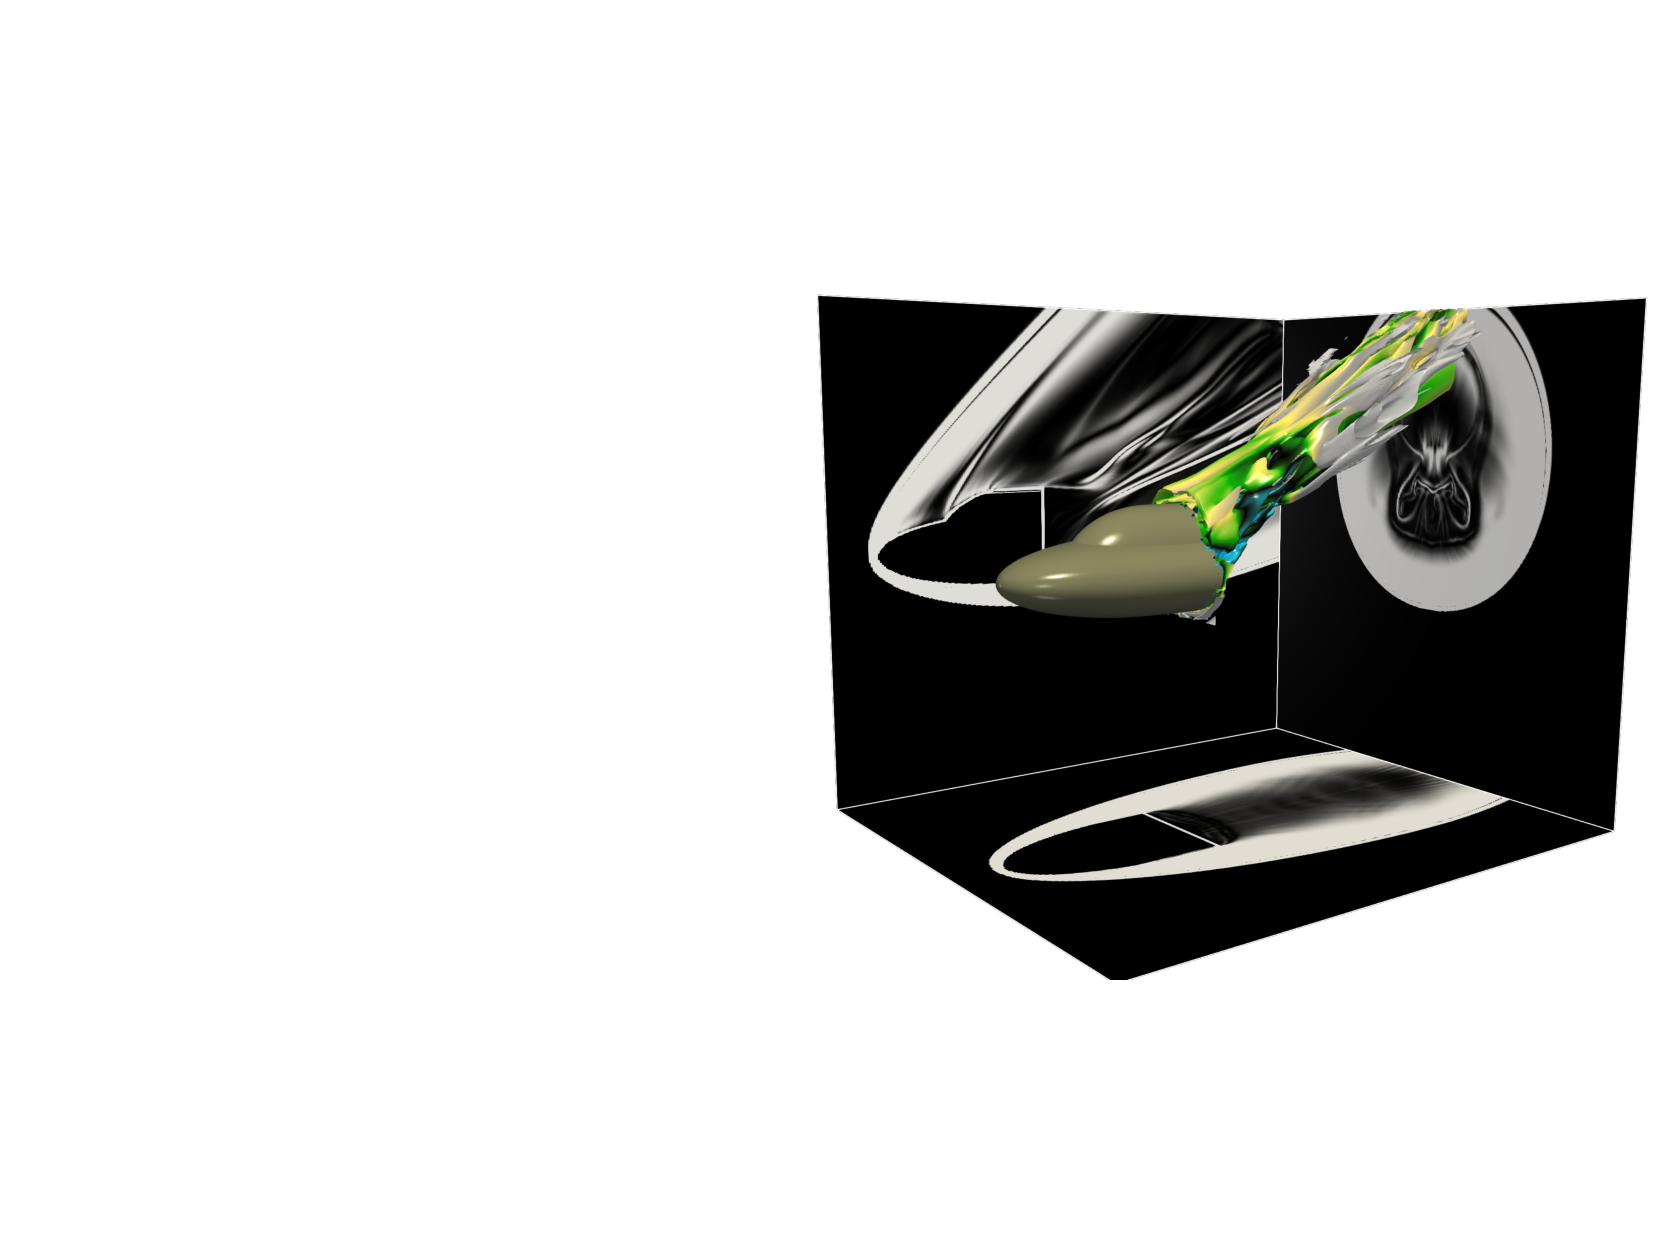
\includegraphics[width=0.65\linewidth]{chapter3_numerical_methods/pictures/ellipse_3Dview.pdf}% &
        % 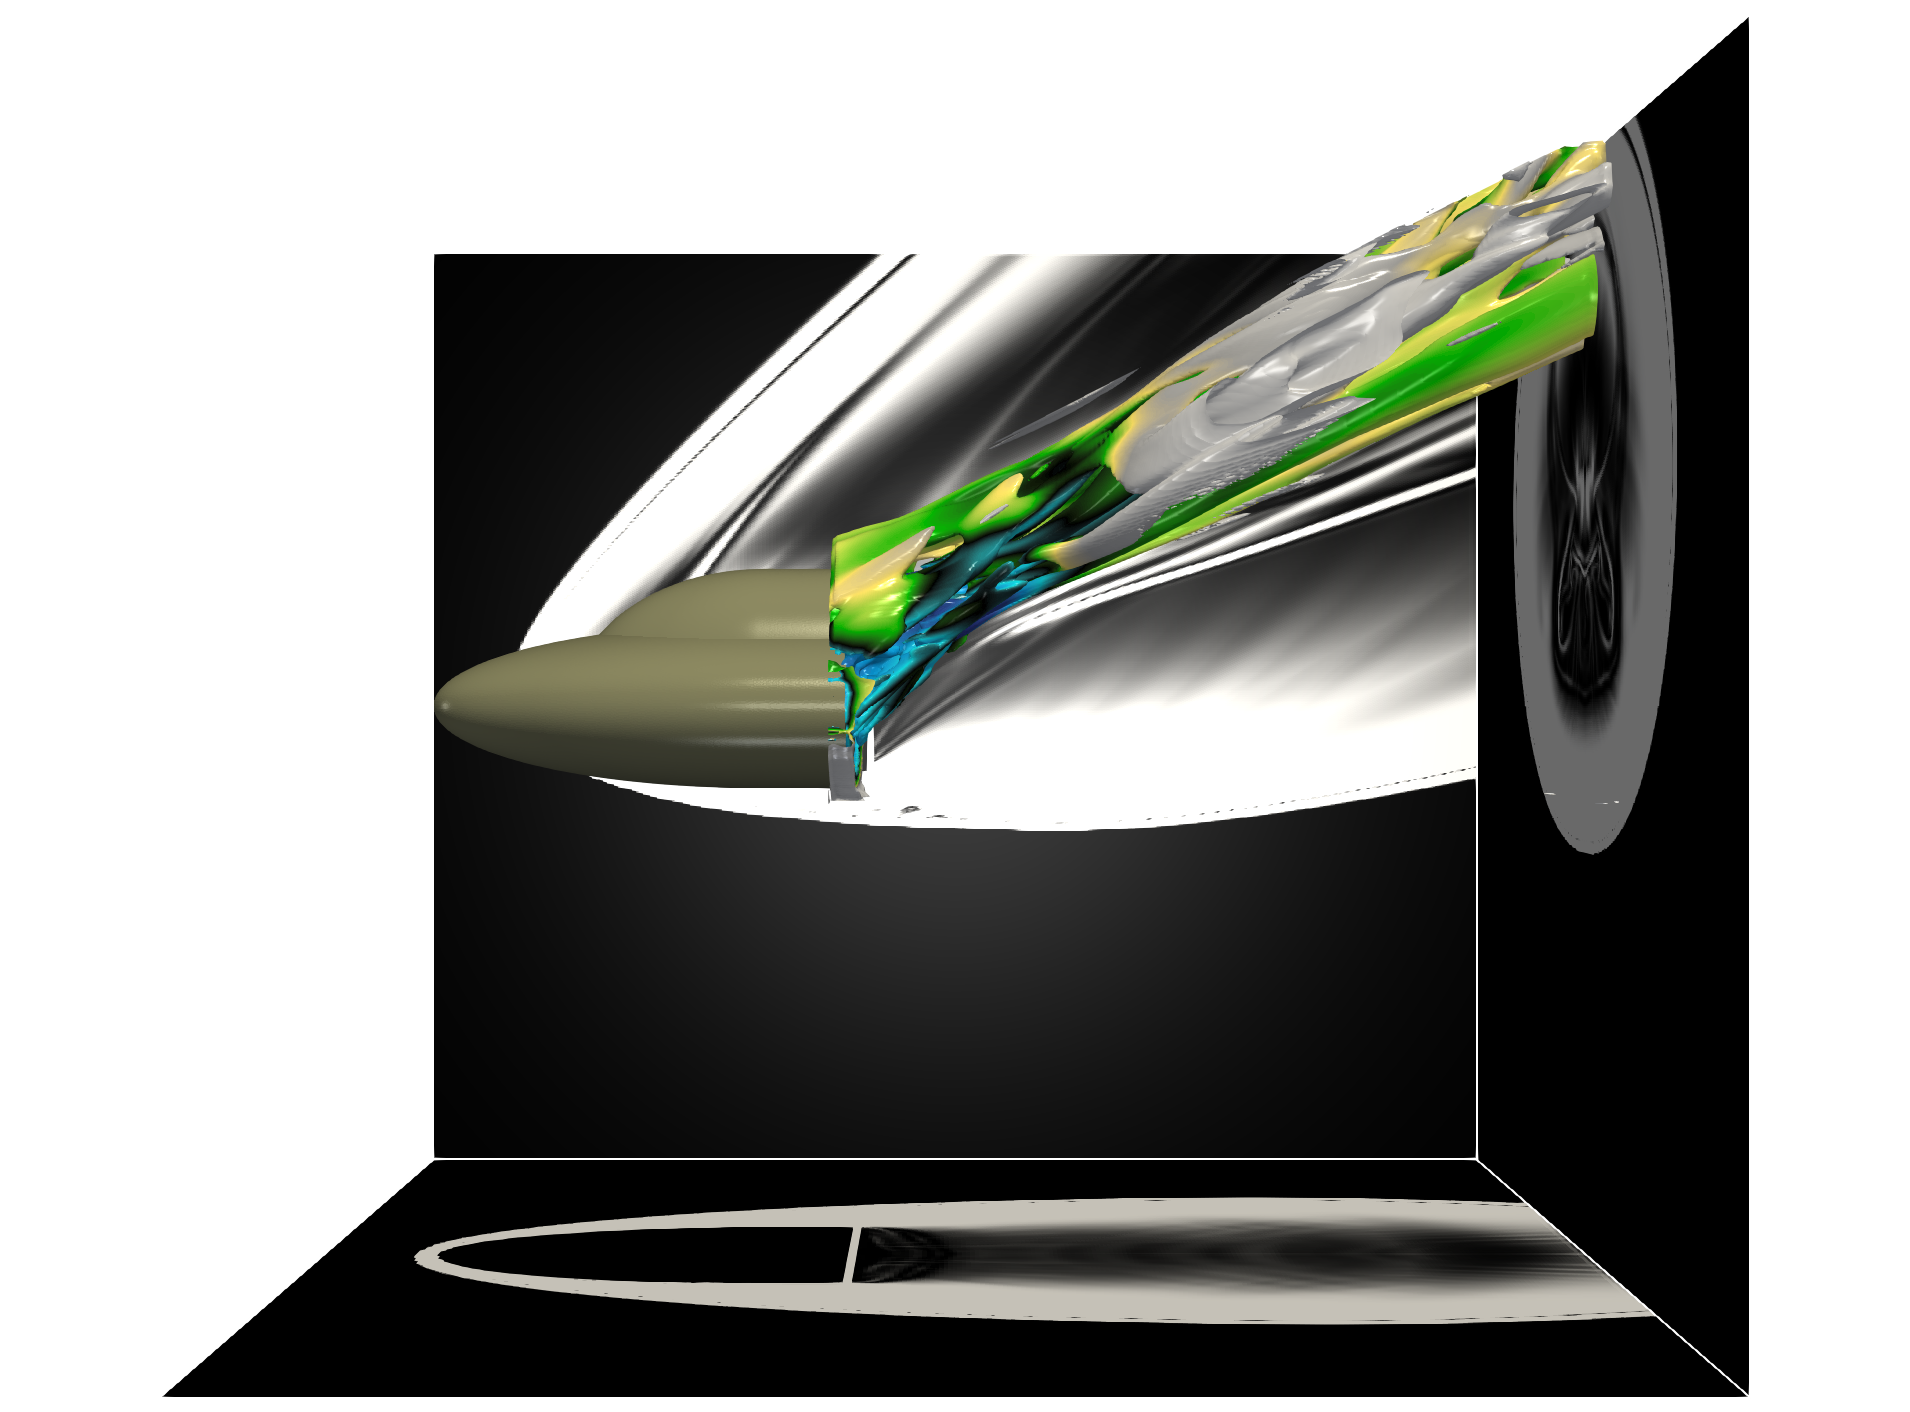
\includegraphics[width=0.45\linewidth]{ellipse_sideview.png}
    % \end{tabular}
    \caption{Illustration of the flow around the double ellipsoid immersed object with a $30^{\circ}$ angle of attack.
    The walls of the visualization domain are colored using the numerical Schlieren imaging technique, and the wake of the double ellipsoid is shown using isocontours of Q-criterion, colored by the magnitude of the vorticity.
    %Both a perspective (left) and a sideview (right) are displayed.
    }
    \label{fig:ellipse_3D}
\end{figure}

Similarly to the study conducted for the previous test case (see paragraph~\ref{ssec:test_double_cone}), figure~\ref{fig:ellipse_comp} presents the pressure coefficient and the Stanton number at the wall of the double ellipsoid.
The conclusions are similar to the ones for the double cone flow.
The pressure coefficient is satisfactorily predicted - the experimental data does not allow to conclude on the nature of the oscillations observed in the vicinity of the recirculation region (when the second ellipsoid starts, around $x \simeq 0.0$).
The heat flux accuracy is however fairly low again, mostly because of the lack of alignment between the Cartesian mesh and the object wall causing the boundary layers to be poorly described.
This phenomenon and possible fixes will be, as aforementioned, explored in a future study.

\begin{figure}[ht!]
    \centering
    \begin{tabular}{cc}
        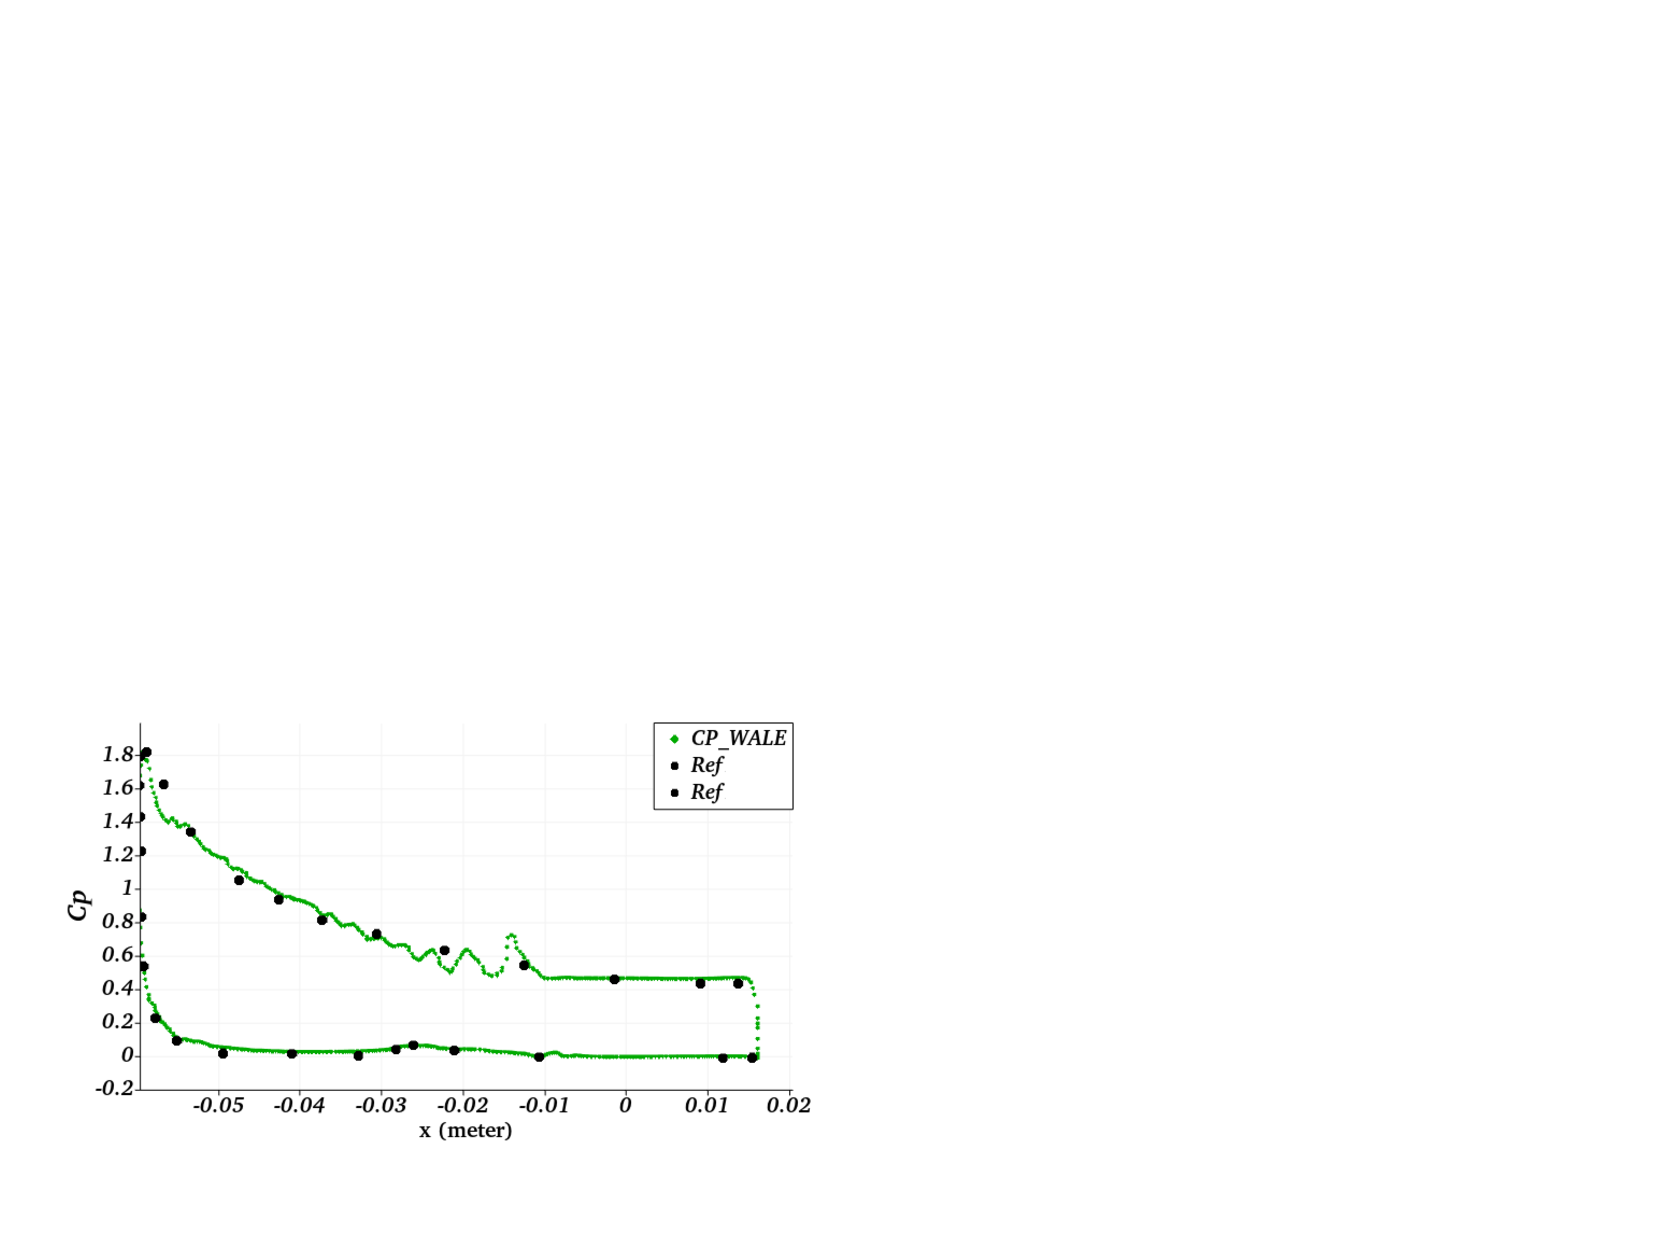
\includegraphics[width=0.45\linewidth]{chapter3_numerical_methods/pictures/ellipse_cp.pdf} &
        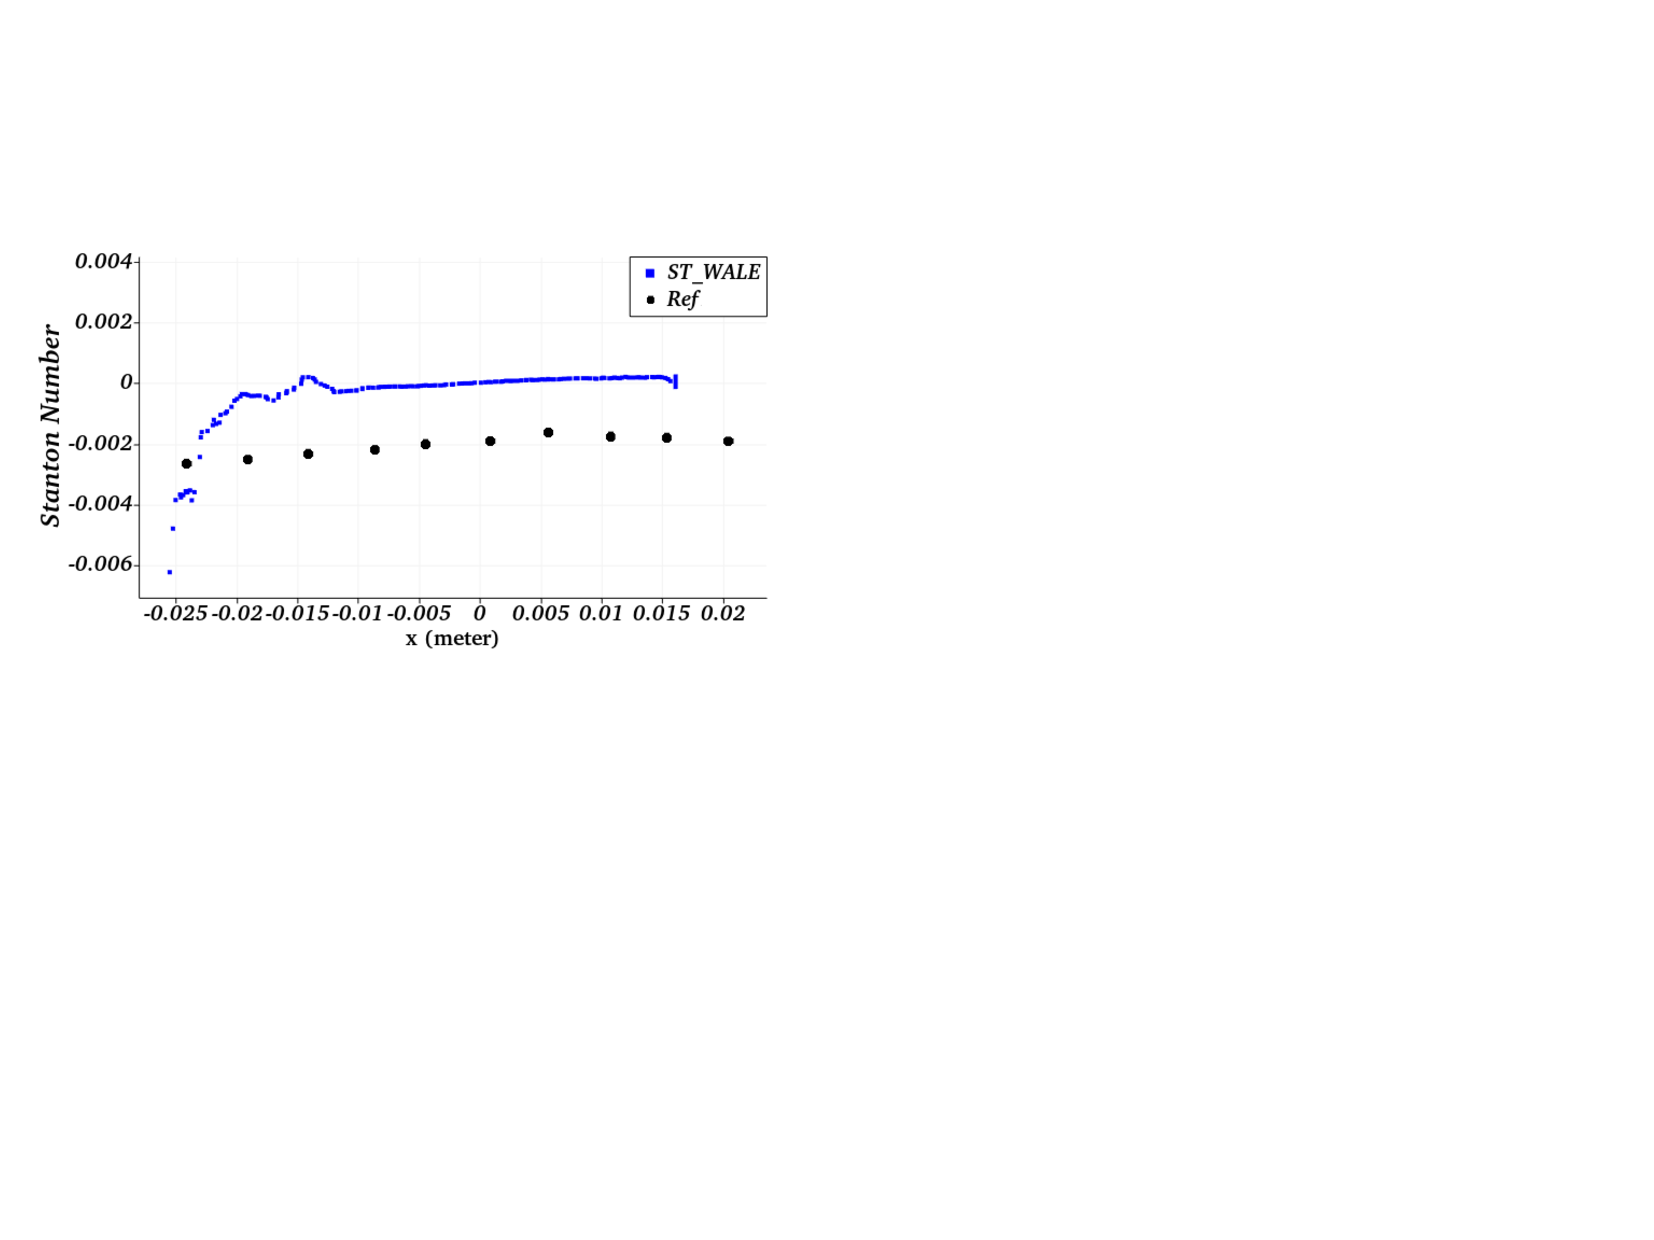
\includegraphics[width=0.45\linewidth]{chapter3_numerical_methods/pictures/ellipse_stanton.pdf} \\
        (a) & (b)
    \end{tabular}
    \caption{(a) Pressure coefficient on both the pressure and the suction sides and (b) Stanton number on the pressure side of the double ellipsoid.
    Comparison between the present computations (green and blue lines) and the experimental reference data (black dots) extracted from \cite{Aymer1991}.}
    \label{fig:ellipse_comp}
\end{figure}


\section{CONCLUSIONS}

In this paper, we present some work related to the immersed boundary method and in particular to the adaption of the method for massively parallel computations.
A novel algorithm based on the theory of computational geometry is introduced to drastically decrease the time necessary to identify a tesselated immersed body in a Cartesian box - from beyond $48$ hours to a few seconds.
The steps of this algorithm are detailed exhaustively and an example implementation of its non-trivial functions is provided.
Still in order to lift major limitations to conducting three-dimensional simulations involving immersed objects on massive clusters, a second algorithm is presented that make the interpolation step of the immersed boundary workflow possible for any number of MPI processes.
This algorithm represents the parallel extension of the works presented in \cite{BRIDELBERTOMEU2021} about an ENO-like least-square reconstruction mandatory to handle strong shocks in the vicinity of immersed bodies subject to hypersonic flows.

As those two new algorithms finally make massively parallel three-dimensional computations accessible with HYPERION, the improvement of the predictive capabilities of the code are then discussed.
Rather than conducting direct numerical simulations that stay, even today, unreachable because of their prohibitive computational cost at high Reynolds numbers, HYPERION is turned towards large eddy simulations (LES).
Preliminary axisymmetric and three-dimensional simulations conducted show that even if adequate subgrid-scale modeling allow for the prediction of large-scale turbulent structures on relatively coarse mesh, it is not enough to capture accurately the near-wall viscous phenomena.
The lack of alignment between the Cartesian grid (fluid grid) and the wall of the immersed body makes for poorly resolved boundary layers which, in turn, yield poor performance when it comes to predicting the viscous-driven wall quantities such as heat flux and shear stress.
A future study shall be dedicated to investigating these shortcomings and proposing solutions, perhaps axed towards the use of wall laws.



\chapter{Topologie}
\begin{figure}[!ht]
 \centering
 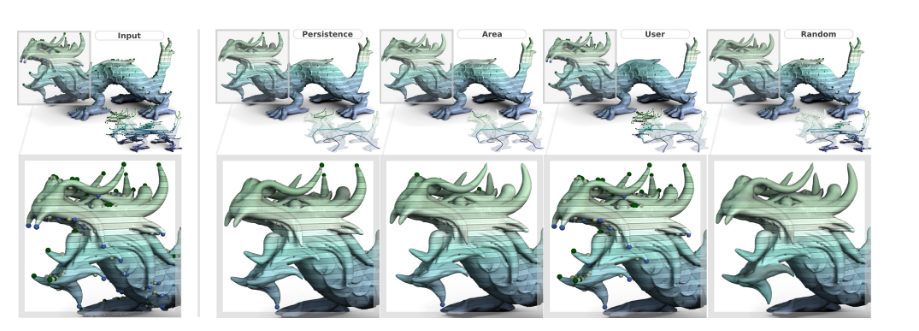
\includegraphics[width=1\linewidth]{chapter4_topology_data_analysis/pictures/picture_chapter.png}
 \vspace{-2ex}
 \caption{IXV spatial navette by esa}
  \vspace{2ex}
 \label{11}
\end{figure}
\minitoc
\thispagestyle{empty}
\newpage


\newcommand{\lt}{<}
\newcommand{\gt}{>}

\newcommand{\discreteMorseFunction}{\mathcal{F}}
\newcommand{\discreteGradientField}{\mathcal{G}}
\newcommand{\discreteVectorField}{\mathcal{V}}
\newcommand{\dimensionality}{d}
\newcommand{\chainGroup}{\mathcal{C}}
\newcommand{\boundaryGroup}{\mathcal{B}}
\newcommand{\cycleGroup}{\mathcal{Z}}
\newcommand{\homologyGroup}{\mathcal{H}}
\newcommand{\persistentHomologyGroup}{\mathcal{PH}}
\newcommand{\domain}{\mathcal{M}}
\newcommand{\stableManifold}{\domain}
\newcommand{\unstableManifold}{\domain'}
\newcommand{\range}{\mathbb{R}}
\newcommand{\sublevelset}[1]{#1^{-1}_{-\infty}}
\newcommand{\superlevelset}[1]{#1^{-1}_{+\infty}}
\newcommand{\Star}{St}
\newcommand{\Link}{Lk}
\newcommand{\simplex}{\sigma}
\newcommand{\face}{\tau}
\newcommand{\lowerlink}{\Link^{-}}
\newcommand{\upperlink}{\Link^{+}}
\newcommand{\Index}{\mathcal{I}}
\newcommand{\offset}{o}
\newcommand{\Natural}{\mathbb{N}}
\newcommand{\criticalSet}{\mathcal{C}}
\newcommand{\diagram}{\mathcal{D}}
\newcommand{\persistentCurve}{\mathcal{C}}
\newcommand{\wasserstein}[1]{W_#1}
\newcommand{\projection}{\Delta}
\newcommand{\hierarchy}{\mathcal{H}}
\newcommand{\decimation}{D}
\newcommand{\xDimD}{L_x^\decimation}
\newcommand{\yDimD}{L_y^\decimation}
\newcommand{\zDimD}{L_z^\decimation}
\newcommand{\xDim}{L_x}
\newcommand{\yDim}{L_y}
\newcommand{\zDim}{L_z}
\newcommand{\Grid}{\mathcal{G}}
\newcommand{\GridD}{\mathcal{G}^\decimation}
\newcommand{\x}{\phantom{x}}
\newcommand{\Mod}{\;\mathrm{mod}\;}
\newcommand{\NN}{\mathbb{N}}
\newcommand{\forwardIntegralLine}{\mathcal{L}^+}
\newcommand{\backwardIntegralLine}{\mathcal{L}^-}
\newcommand{\triangulationOp}{\phi}
\newcommand{\decimationOp}{\Pi}
\newcommand{\isovalue}{w}
\newcommand{\persistence}{\mathcal{P}}
\newcommand{\pointMetric}[1]{d_#1}
\newcommand{\diagramSet}{\mathcal{S}_\mathcal{D}}
\newcommand{\diagramSpace}{\mathbb{D}}
\newcommand{\jointree}{\mathcal{T}^-}
\newcommand{\splittree}{\mathcal{T}^+}
\newcommand{\mergetree}{\mathcal{T}}
\newcommand{\mergetreeSet}{\mathcal{S}_\mathcal{T}}
\newcommand{\branchset}{\mathcal{S}_\mathcal{B}}
\newcommand{\branchspace}{\mathbb{B}}
\newcommand{\mergetreeSpace}{\mathbb{T}}
\newcommand{\editdistance}{D_E}
\newcommand{\wassersteinTree}{W^{\mergetree}_2}
\newcommand{\distanceSequence}{d_S}
\newcommand{\branchtree}{\mathcal{B}}
\newcommand{\branchtreeSet}{\mathcal{S}_\mathcal{B}}
\newcommand{\branchtreeSpace}{\mathbb{B}}
\newcommand{\forest}{\mathcal{F}}
\newcommand{\sequenceSpace}{\mathbb{S}}
\newcommand{\forestMatrix}{\mathbb{F}}
\newcommand{\treeMatrix}{\mathbb{T}}
\newcommand{\normalizedLocation}{\mathcal{N}}
\newcommand{\normalizedWasserstein}{W^{\normalizedLocation}_2}
% \newcommand{\normalizedTree}{N}

\newcommand{\note}[1]{\textcolor{magenta}{#1}}
\newcommand{\cutout}[1]{\textcolor{blue}{#1}}
\renewcommand{\cutout}[1]{}



\newcommand{\eqSpace}{\vspace{-.5ex}}
\newcommand{\figureShrink}{0.9915}

\newcommand{\mycaption}[1]{
\vspace{-2ex}
\caption{#1}
\vspace{-2ex}
}

\section{Introduction}

\begin{figure}
 \centering
%  \vspace
 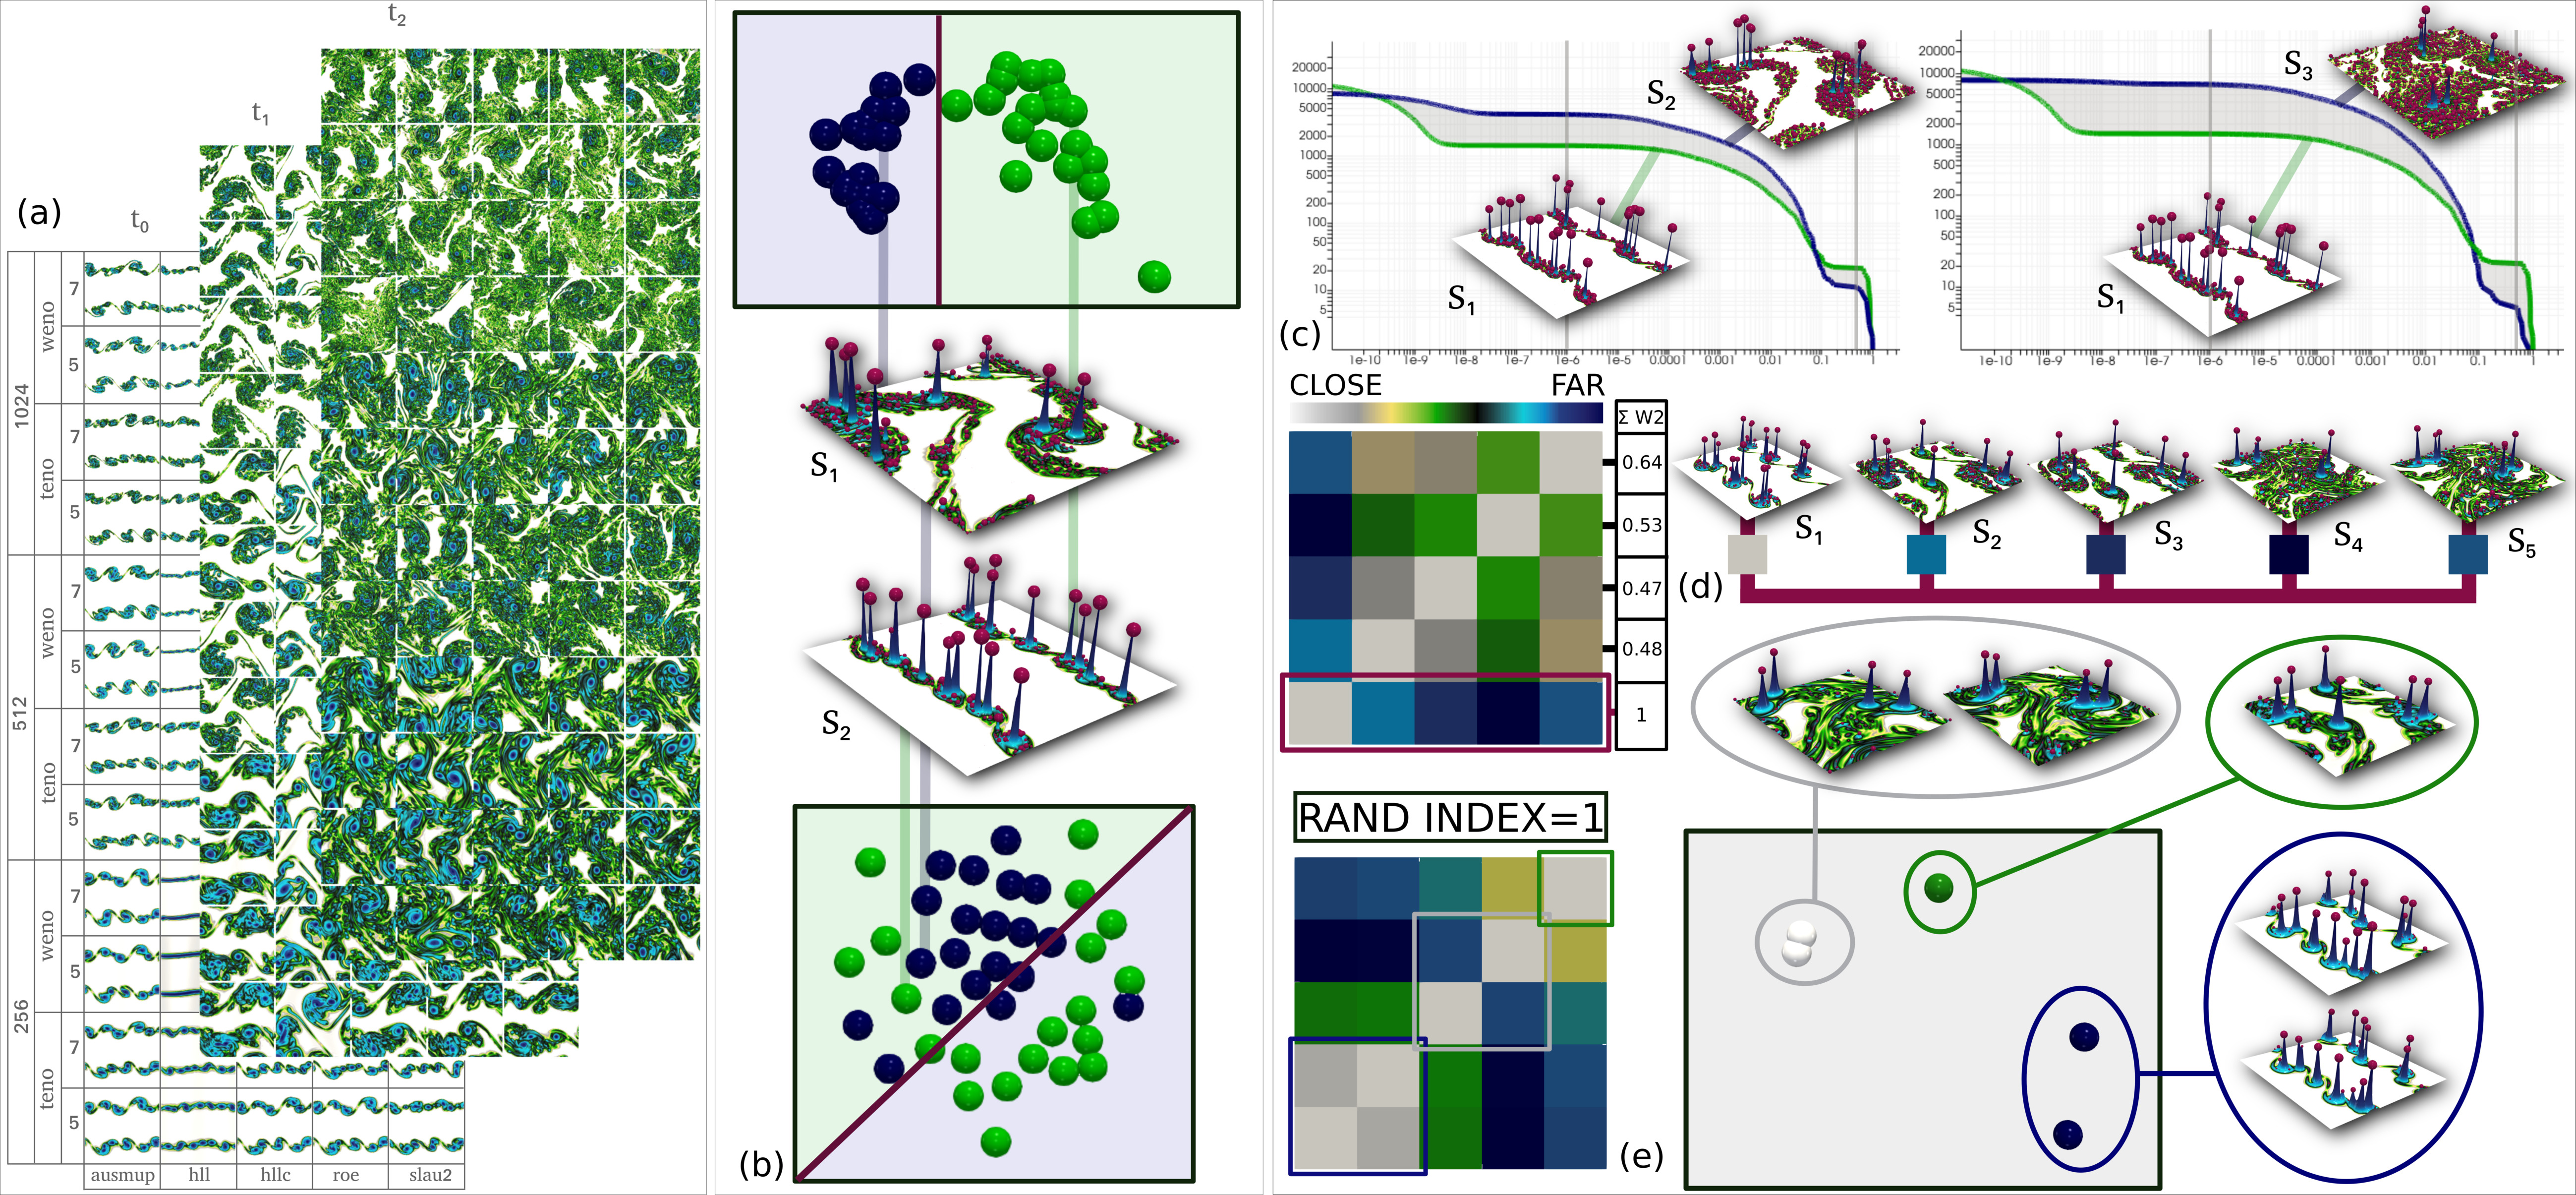
\includegraphics[width=1\linewidth]{chapter4_topology_data_analysis/pictures/teaser2.jpg}
 \caption{ Data Analysis protocols
%   to illustrate the segmentation
applied
  on an ensemble dataset of a Kelvin-Helmholtz instability.
(a) The 180 members of the ensemble obtained with variations of timesteps, interpolation schemes, orders, resolutions and Riemann solvers (\autoref{tab_parameters}).
(b) The top cluster represents the time separation of $t_0$ and $t_1$ for the
flows $S_1$ and $S_2$ with the Wasserstein distance and the bottom cluster with
the $L_2$-norm. Red lines show the timestep separation with our clustering
method whereas the sphere colors are the ground truth, illustrating the
limitation of the $L_2$-norm.
(c) \textit{Persistence curve protocol}: Differences between integrals of persistence curves (gray area) of the enstrophy computed with a SLAU2 solver, an order 7 TENO scheme and a resolution of $1024\times 1024$ for various configurations ($S_1$ at $t_0$, $S_2$ and $S_3$ at $t_1$). These integral differences exhibit the appearance of vortices (critical points) as the time increases.
(d) \textit{Outlier distance protocol}: Wasserstein distance matrix for 5 configurations $S_1(t_0,HLLC)$, $S_2(t_1,Roe)$, $S_3(t_1,HLLC)$, $S_4(t_2,Roe)$, $S_5(t_2,HLLC)$ computed with an order 7 WENO-Z interpolation scheme at $512\times 512$.
The sum of each row
% allows us to identify
the configuration maximizing this distance between solvers and timesteps, here $S_1$.
(e) \textit{Unsupervised classification}: Wasserstein distance matrix for the
previous configurations with an order 7 WENO-Z interpolation scheme at
$256\times 256$. The clustering based on the Wasserstein distance and colored
according to the Kmeans clustering method successfully segments the time
steps.}
 \label{fig_teaser}
\end{figure}

Flow turbulence is a phenomenon of major importance in fluid dynamics.
It is characterized by chaotic changes in the motion of a flow (\emph{e.g.}
typical cigarette smoke patterns), which have a drastic impact in numerous
applications (aeronautics, weather forecast, climate modeling, material
sciences, astronomy, etc.).
Although turbulence has been studied since the early stages of modern physics,
its theoretical mastery remains incomplete \cite{baez2006} and the
understanding of the
Navier-Stokes equations, central
in the description of
% to
fluid motion, is still
considered as
a
% one of the
major open challenge in mathematics and physics,
as proven by the Clay Mathematics Institute selecting it to be
% and
% has been selected by
among its celebrated Millennium Prize problems \cite{fefferman2000}.
Thus, in engineering applications, the main practical solution available for
the study of turbulence
% and turbulent flows
remains numerical simulation.

\noindent
\textbf{Problem introduction:}
However,
% plenty of
many
different numerical solvers can be used to simulate a given flow configuration, each
solver being itself subject to several input parameters (such as domain
resolution, interpolation scheme and order, etc.): when faced with such a wide variety,
% \julien
the main problem for users becomes
the configuration itself of the simulation parameters.
% to choose the right solver.
% Then, the problem of evaluating and comparing the performance of different solver configurations is
% of major importance.
In particular, domain experts want not only to identify
the solver configurations which produce the most realistic simulations, but
they also want to discover configurations resulting in
degraded but fast
% fast, degraded
computations, which still produce simulations of acceptable realism. The
fundamental problem behind such comparative analyses is that of comparing
\emph{quantitatively} turbulent flows. For instance, the quantitative realism
of a simulation could be evaluated by comparing its outcome to a reference,
either obtained by acquisition or by a highly detailed simulation considered as
a ground-truth. However, the chaotic nature of turbulent flows makes their direct
comparison with standard imaging tools
% (\emph{e.g.} the $L_2$ norm, \autoref{fig_teaser})
impractical. For instance, turbulent flows which are considered similar at a
high level by domain experts (in terms of the number and size of their vortices)
are reported by classical metrics such as the $L_2$ norm as being very distant
(\autoref{fig_teaser}), as such pointwise measures are sensitive to mild
geometrical variations in the data and miss global structural
similarities in such a chaotic context. This observation motivates the
consideration of alternative similarity estimation tools, which focus on the
\emph{structure} of the flow, rather than its raw geometry.

In that regard, Topological Data Analysis (TDA) \cite{edelsbrunner09} forms a
family of generic, robust and efficient techniques, whose purpose is precisely
to recover hidden implicit structural patterns in complex data, and to enable
their reliable representation and comparison. As such, they provide
potentially relevant alternatives to standard comparison measures used in
scientific imaging, such as the $L_2$ norm. Moreover, the utility of TDA has
been already demonstrated in a number of analysis and visualization tasks
\cite{heine16}, with examples of successful applications in
combustion \cite{laney_vis06, bremer_tvcg11, gyulassy_ev14},
material sciences \cite{gyulassy_vis07, gyulassy_vis15, favelier16},
% fluid dynamics \cite{kasten_tvcg11},
bioimaging \cite{carr04, topoAngler, beiBrain18},
quantum chemistry \cite{chemistry_vis14, harshChemistry, Malgorzata19}, or
astrophysics \cite{sousbie11, shivashankar2016felix}. In
particular, the critical points of flow vorticity indicators have been
reported to appropriately capture the center of vortices \cite{kasten_tvcg11,
bridel_ldav19}, as well as their importance, with the notion of
\emph{topological persistence} \cite{edelsbrunner02}. Such  results provide
additional evidence and consolidate the intuition that TDA could be a
relevant framework for comparing turbulent flows.

The ambition of this application paper is to provide a comprehensive
experimental evaluation of
% experimentally
% evaluate
the above intuition, i.e. to assess the suitability of
topological data representations and their associated analysis tools for the
quantitative comparisons of turbulent flows.
%We shall focus on a peculiar type of turbulence that expresses itself in two dimensions (akin to the soap-film turbulence displayed in Fig.~\ref{fig:soapfilm}): it is a fair representative of generic turbulence (\emph{a.k.a.} three-dimensional viscous turbulence) and allows for affordable high-resolution simulations to feed our study.
We shall focus on a specific type of turbulence that expresses itself in two dimensions (Kelvin-Helmholtz instability): it is a fair representative of generic turbulence (\emph{a.k.a.} three-dimensional viscous turbulence) and allows for affordable high-resolution simulations to feed our study.
% Image du SAVON
%\begin{figure}
%    \centering
%    \includegraphics[width=0.75\linewidth]{turbulenceinasoapfilm_cut.jpeg}
%    \caption{Experimentally generated, gravity-driven, turbulent soap film.Interference fringes in yellow light (wavelength = 0.589 µm) make it possible to visualize the generation of 2D turbulence\cite{tran2010macroscopic}.Color-reproduction courtesy of Okinawa Institute of Science and Technology.}
%\label{fig:soapfilm}
%\end{figure}
Specifically, our study documents
the usage of the persistence diagram of the maxima of flow enstrophy (an established indicator of vorticity for two-dimensional flows,
\autoref{sec_background}) for the topological representation of 180 members of
an ensemble of hydrodynamic turbulent flows, generated by a coarse sampling of
the parameter space of five distinct solvers.
We document five main hypotheses (\autoref{sec_caseStudy}) reported by domain
experts, describing their expectations with regard to the variability among the
flows generated by the distinct solver configurations.
Then, we describe three evaluation protocols (\autoref{sec_protocols}) designed
to assess the validation of the above hypotheses by standard comparison
measures ($L_2$ norm) on one hand, and by topological methods on the other.
Specifically, these protocols exploit the persistence curve, the
$L_2$-Wasserstein distance between persistence diagrams \cite{Turner2014} and
$k$-means in the $L_2$-Wasserstein metric space \cite{vidal_vis19}. Finally, we
document
the
results of these
% evaluation
protocols on the input ensemble
% , are
% documented
% and the corresponding insights are discussed
(\autoref{sec_experimentalResults}). We believe that the insights reported by
our study bring a strong experimental evidence of the suitability
of TDA for representing and comparing turbulent flows, thereby providing
confidence in its usage by the fluid dynamics community in the future.
Moreover, our flow data and evaluation protocols provide to the TDA community
an application-approved benchmark for the evaluation and design of further
topological distances in the future.

% can be used as a justification in future work.

% While several, global indicators are
% established in the computational fluid dynamic community (such as energy plots
% as function of wave numbers, \autoref{sec_relatedWork})

% \julien{One sentence to explain why they are difficult to study.}
% \julien{One sentence explaining the vast possibilities in terms of solver
% and parameters and the difficulty to tune them.}
% \julien{One sentence explaining that existing quality metrics and their
% limitations: they are global, they don't take into account subtle behaviors,
% this is a problem when increasing the resolutions because vortices have a
% very restricted spatial support (hence their contribution impact modestly
% aggregative quality metrics).}
% \julien{One sentence to explain that two ensemble members are rather hard to
% compare, since two similar flows from a fluid mechanics point of view, can be
% highly dissimilar visually, which challenges standard metrics such as the $L_2$
% norm. This motivates more advanced tools capable of extracting features of
% interest and compare them directly.}
% \julien{One sentence to announce that in this work, we perform an exhaustive
% experimental study to evaluate the relevance of topological data
% representations for the evaluation and comparisons of solvers of hydrodynamic
% turbulent flows.}
% \julien{One sentence to explain quickly what topological data representations
% are about and in which context they have been used. Finish on recent work
% suggesting to compare them and study them at a statistical level. We exploit
% these recent advances in our current work.}
% \julien{Brief overview of the kinds of study we're going to show
% (\autoref{sec_protocols}): (i) comparisons of persistence curves, (ii)
% Wasserstein distances between persistence diagrams, (iii) Clustering in the
% Wasserstein metric space.}
% \julien{An exhaustive analysis on an ensemble of 180 members
% \autoref{sec_experimentalResults} validate the ability of topological
% descriptors to discriminate better different regions parameter space, and
% reveal  new insights on hydrodynamic turbulent flow simulations.}

% \vspace{-1ex}
\begin{figure}
 \centering
%  \vspace
 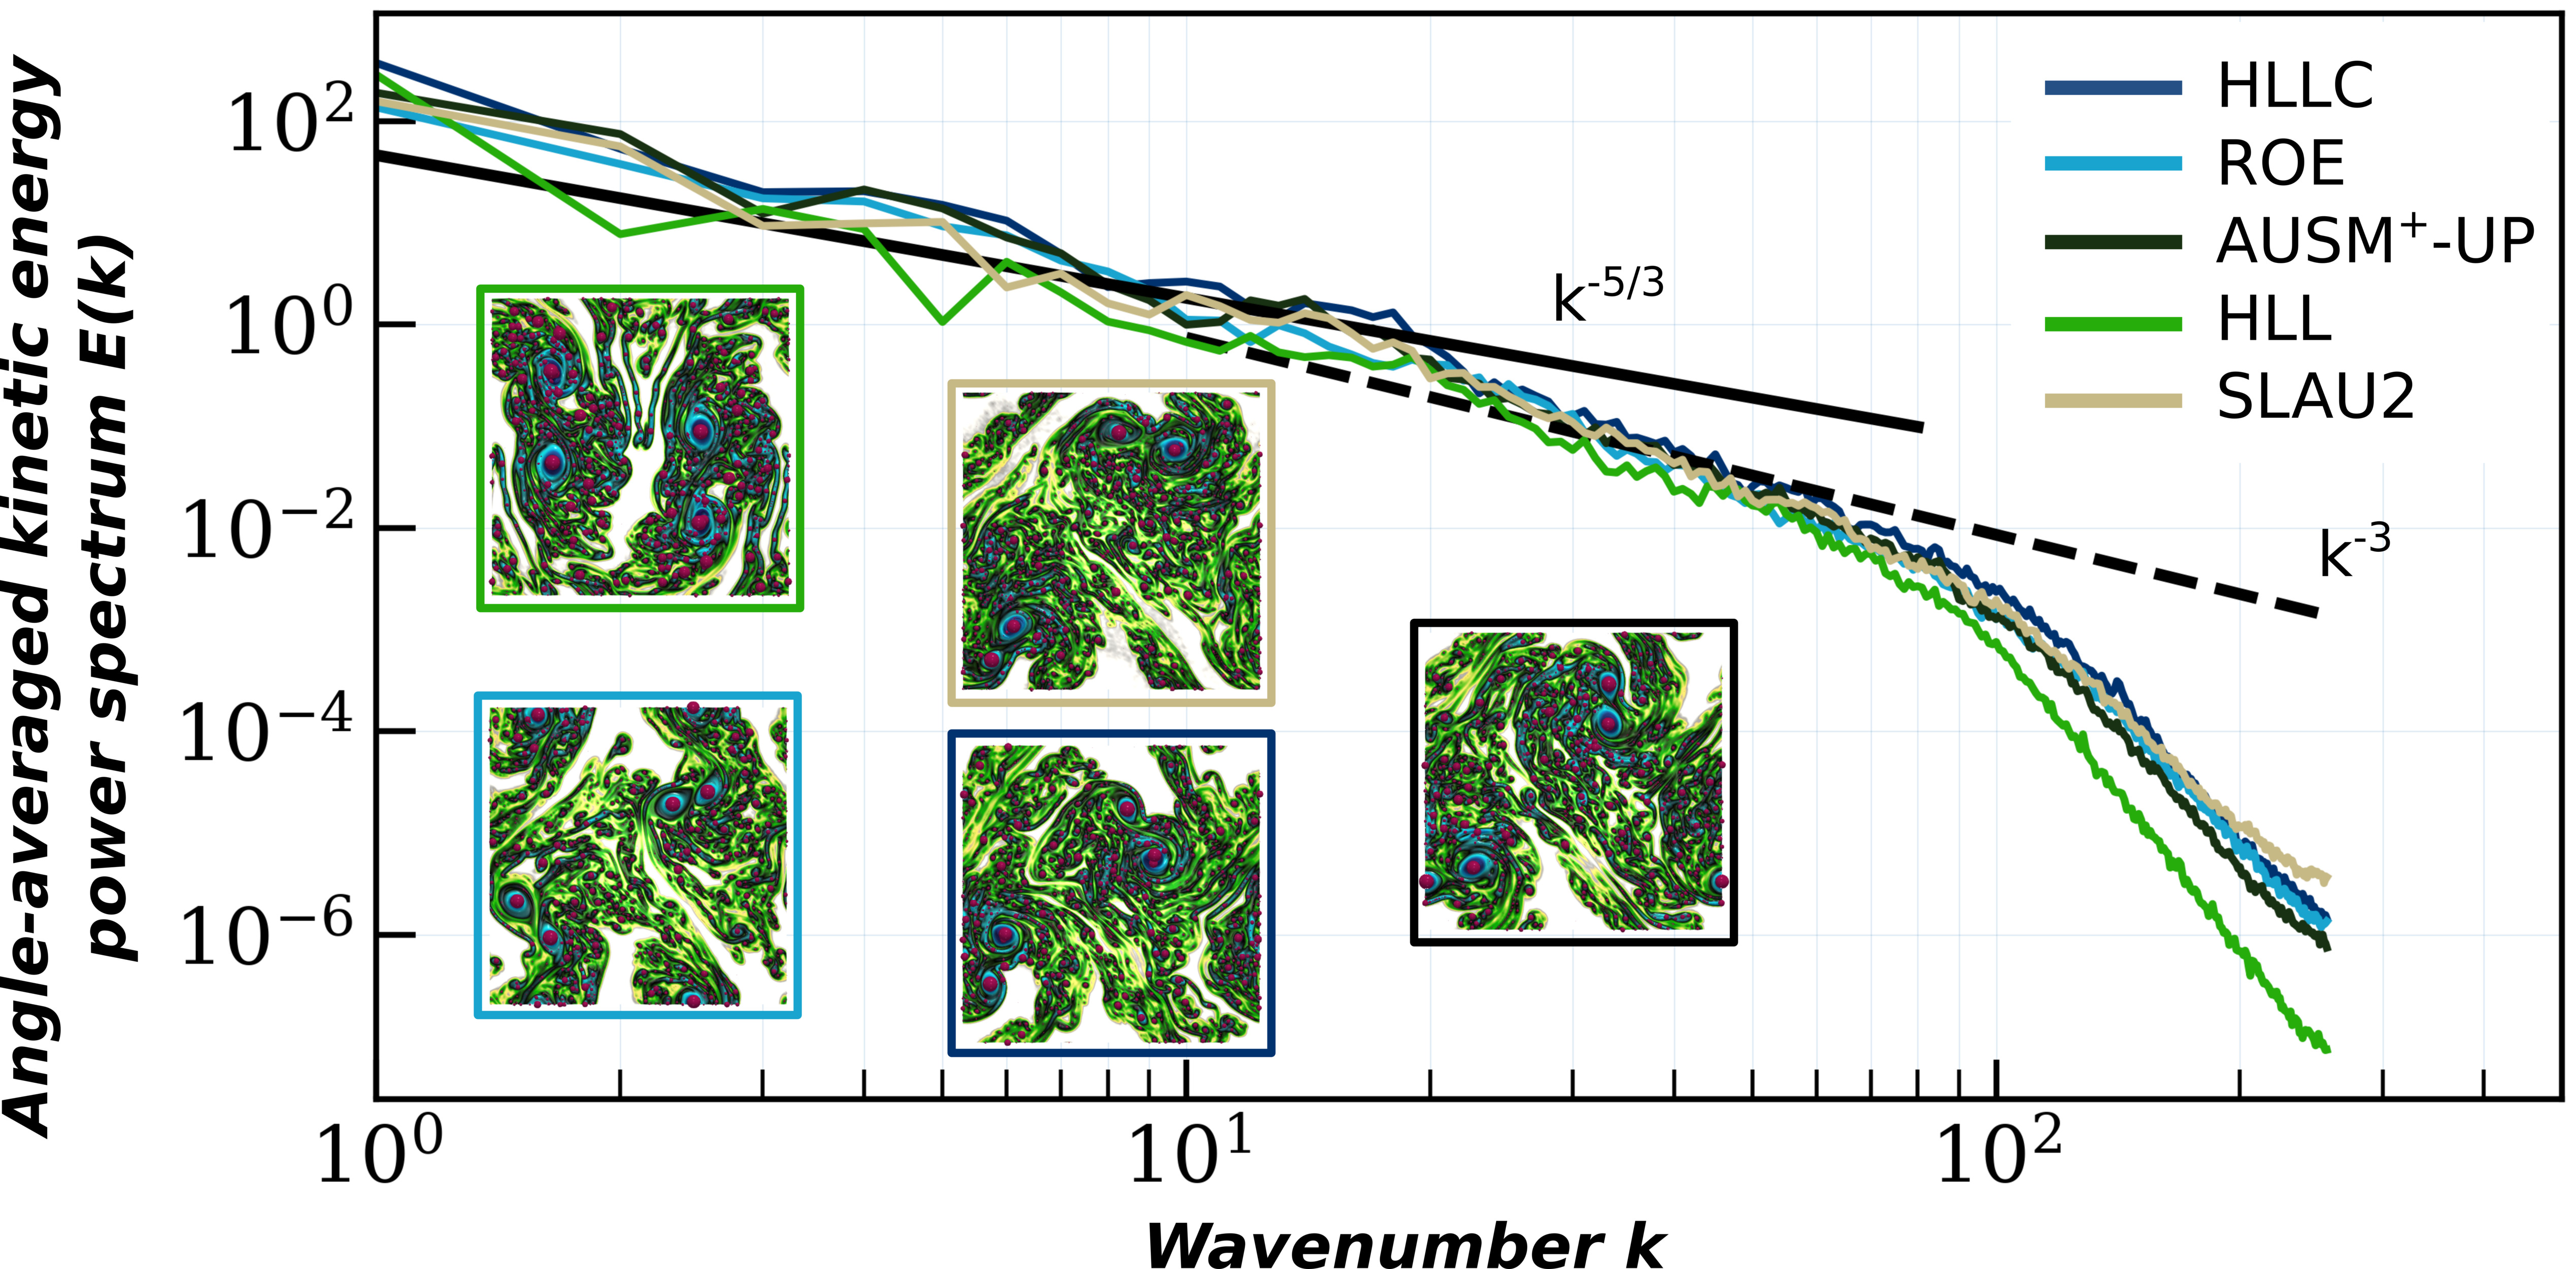
\includegraphics[width=\linewidth]{chapter4_topology_data_analysis/pictures/energie.jpg}
 \mycaption{Baseline analysis by angle-averaged kinetic energy power spectrum
 for all solvers (WENO-Z, order $7$, $t_2$, $512\times512$).
%  with the WENO-Z seventh order, at $t_2$, with 512 x 512 cells for all solvers.
 }
 \label{energie}
\end{figure}

\subsection{Related work}
\label{sec_relatedWork}
This section presents the literature related to our work.
First, we
 discuss previous work dealing with \emph{(i)} simulations of turbulent
flow
% as well as
and their quantitative evaluation. Next, \emph{(ii)} we review
previous work dealing with topological methods for the analysis of ensemble
data.

\noindent
\textbf{\emph{(i)} Turbulent flow simulation.}
% \julien{todo:
% \begin{enumerate}
%  \item Faire un bref historique des références clés pour la simulation
% d'écoulements turbulents
%  \item Faire un bref historique des méthodes clés pour évaluer quantitativement
% la qualité d'un écoulement.
% \end{enumerate}
% }
Turbulence is ubiquitous in nature, at all scales, from Higgs-Boson condensates \cite{Kraichnan1967} to a stirred cup of coffee to geophysical flows \cite{Kraichnan1980} to galaxy formation.
While a significant literature in graphics \cite{KimTJG08, ZhangLSSQ14, BaiWDL21} focused on the efficient generation of visually plausible turbulence, we focus in this work on the direct numerical simulation of the underlying physical equations, for engineering applications.
% One motivation to study turbulence, and in particular two-dimensional turbulence, shared by all investigators is that despite its practical applications, its omnipresence and the years of scrutiny it was subjected to, remains one of the most important unsolved problems of classical mechanics.
A special distinction of 2D turbulence is that it is never realized in nature that, unless strongly constrained,
%\cite{Danilov2002},
always has some degree of three-dimensionality but rather it only exists in computer simulations.
Two-dimensional turbulence has thus been studied extensively by the latter means \emph{e.g.} for its importance as an idealization of meteorological flows \cite{Boffetta2011}, its role in the confinement of thermonuclear plasmas \cite{Kraichnan1980} but also as a cost-effective numerical testing ground for three-dimensional flows dynamical theories \cite{Tabeling2002}.
Most such studies focus either on validating predictions of theorists \cite{Kraichnan1967,lilly1989two} or on providing insights into the dynamic behavior of 2D eddies thanks to high-resolution simulations \cite{lilly1989two,Maltrud1991}.
The simulations are usually analyzed by considering macroscopic quantities such as the enstrophy (see below equation~\eqref{eq:enstrophy}), or by considering the Fourier decomposition of the 2D field (similar to \autoref{energie})- integral indicators that make it near impossible to compare and/or classify the results of, say, a parametric study.
% These classical indicators all integrate the data to some extent and, faced with two numerical realizations produced using different numerical settings, make it near impossible to classify the results.
Some efforts have been made recently \cite{san2015evaluation} to provide the users with some guidelines to best choose the numerical methods and parameters for the simulation of 2D turbulence, but still using, mostly, the aforementioned integral, inaccurate, indicators.
The present study aims at providing the workers in 2D turbulence with another tool to classify their results and best choose their settings, this time using mostly local indicators able to exploit the whole flow.

\noindent
\textbf{\emph{(ii)} Topological methods for ensemble analysis.}
Concepts and algorithms from computational topology \cite{edelsbrunner09} have
been investigated, adapted and extended by the visualization community for more
than twenty years \cite{heine16}. Specifically, a large body of literature has
been dedicated to the analysis and visualization of flow data with
topological methods and we refer the readers to a series of surveys on the topic
\cite{ScheuermannT05, GarthT06,
LarameeHZP07, PobitzerPFSKTMH11,
wang2016,
BujackYHGW20},
including a
recent iteration \cite{flowIntro21}.
A substantial line of work
\cite{petz, otto2, otto1} focused on extending topological techniques to
uncertain vector fields, where flow variability is encoded via a pointwise
estimator (\emph{e.g.} an histogram) of an \emph{a priori} vector distribution, but only few
techniques explicitly focused on the analysis of flow variability in an
ensemble.
Specifically, several comparative visualization techniques have been
proposed \cite{filip3, schneider2012,Hummel2013, GuoHPSCH16, JaremaKW16, filip2, filip1, LohfinkG20}. Ferstl et al.
\cite{Ferstl2016} investigated the global structure of flow ensembles, by
proposing a  clustering approach of the  members, based on a measure of
streamline similarity.
However, these techniques assume a mild
geometrical variability within the ensemble and are therefore
% are
not suited to highly
turbulent flows as studied in this work, where the geometry of the features
(streamlines, vortices) chaotically changes from one ensemble
member to the other (\autoref{fig_teaser}), even upon only slight variations of
the simulation input parameters.
In certain application contexts, CFD experts often prefer to focus their analysis on (simpler to interpret) scalar descriptors generated from the flow, such as the kinetic energy (\autoref{energie}) or the enstrophy (\autoref{eq:enstrophy}). Such a transition to a scalar descriptor enables them to leverage the existing tools for scalar data analysis.
% In several applications, the features of interest in the flow can be reliably
% represented by considering a single pointwise scalar descriptor, such as
% pressure, energy or an estimation of vorticity for instance.
% Such a transition to a scalar descriptor of the flow enables users to leverage
% the ensemble of existing tools for scalar data analysis.
For instance, several
authors \cite{kasten_tvcg11, bridel_ldav19} have shown that, given a relevant
vorticity scalar descriptor, the center of the flow vortices could be reliably
extracted and tracked over time, which supports the idea that
topological methods for scalar data can be useful for the description of
specific flow features. Thus, in the following, we describe the literature
related to topological methods for scalar data.
Popular topological representations include the persistence diagram
\cite{edelsbrunner02, edelsbrunner09}
% (\autoref{fig_mergeTree}),
which represents the
population of features of interest in function of their salience, and which
can be computed via matrix reduction
\cite{edelsbrunner09, dipha}. The Reeb graph \cite{biasotti08}, which describes
the connectivity evolution of level sets, has also been widely studied and
several efficient algorithms have been documented \cite{pascucci07,
tierny_vis09, parsa12, DoraiswamyN13}, including parallel algorithms
\cite{gueunet_egpgv19}.
Efficient algorithms have also been documented for its variants,
% including
the
merge and contour trees \cite{tarasov98, carr00}
and parallel algorithms have
also been described \cite{MaadasamyDN12, AcharyaN15,
CarrWSA16, gueunet_tpds19}. The Morse-Smale complex \cite{EdelsbrunnerHZ01,
EdelsbrunnerHNP03,
BremerEHP03}, which depicts the
global behavior of integral lines, is another popular topological data
abstraction in visualization \cite{Defl15}. Robust and efficient algorithms
have been introduced for its computation  \cite{robins_pami11, ShivashankarN12,
gyulassy_vis18} based on Discrete Morse Theory \cite{forman98}.
Inspired by the literature in
optimal transport \cite{Kantorovich, monge81}, the Wasserstein distance between
persistence diagrams \cite{edelsbrunner09}
(and its variant the
Bottleneck distance \cite{edelsbrunner02}) have been extensively studied.
% This distance
% is based on a bipartite assignment problem.
In
practice, it enables users to compare ensemble members based on their
persistence diagrams.
In our experimental study, we focus on this first, established topological tool
for comparing the topology of ensemble members and we refer the reader to a
recent survey \cite{YanMSRNHW21} for a description of alternative metrics
between topological descriptors.
Several techniques have been proposed for summarizing the topological features
in an ensemble or analyzing their variability.
% For instance,
Favelier et al.
\cite{favelier2018} and Athawale et al. \cite{athawale_tvcg19} introduced
approaches for analyzing the variability of critical points and
gradient separatrices respectively. Recent approaches aimed at summarizing
an ensemble of topological descriptors by computing a notion of \emph{average}
% topological
descriptor,
% with respect to
given a specific metric.
% Such a
This notion has
been well studied for persistence diagrams \cite{Turner2014,
lacombe2018, vidal_vis19}, with direct applications to ensemble clustering
\cite{vidal_vis19}, and analogies have been developed for merge
trees \cite{YanWMGW20, pont_vis21}.
%
% - scalar data ensemble analysis (cite previous work on ensemble)
% % (\autoref{sec_background_persistenceDiagrams}),
% % for which exact
% % \cite{Munkres1957} and approximate \cite{Bertsekas81, Kerber2016}
% % implementations are publicly available \cite{ttk17}.
%
% These building blocks have been well studied
% for persistence diagrams
% barycenters of diagrams
% \cite{Turner2014,
% lacombe2018, vidal_vis19}.
% analogies recently developed for merge trees \cite{YanWMGW20, pont_vis21}.
%
%
% \julien{Related work in topology, applications to various fields including flow
% analysis.}

% \fabien{Test}
% \florent{Test2}


\subsection{Contributions}
This application paper makes the following new contributions:
\vspace{-1ex}
\begin{enumerate}[itemsep=-0.75ex]
 \item{\emph{An evaluation procedure for distances between turbulent
flows:}
 We document 5 main hypotheses reported by domain experts, describing their
expectations
about
% regarding
flow variability
within the studied ensemble (180 members).
We contribute 3 evaluation protocols,
to assess
the validation of the
hypotheses by a specific metric,
given as a distance matrix between the members;}
 \item{\emph{A comprehensive experimental study:}
 We provide a detailed experimental study of the ensemble under consideration
for two distance metrics: \emph{(i)} a standard distance used in scientific
imaging (the $L_2$ norm) and \emph{(ii)} an established topological distance
between persistence diagrams (the $L_2$-Wasserstein metric). Our
experiments demonstrate the superiority of the topological distance to report
as close solver configurations which are expected to be similar by domain
experts. The insights reported by our study bring an experimental evidence
of the suitability of the persistence diagram for representing and comparing
turbulent flows, thereby providing to the fluid dynamics community confidence
for its usage in future work;}
 \item{\emph{An application-approved benchmark:}
 We provide as supplemental material \emph{(i)} the input ensemble of 180
turbulent flows (see \cite{data} for a direct link)
% as well as
and
%\emph{(ii)} Python scripts for reproducing our results.
%Our scripts support the usage of custom distance matrices, thereby providing to the TDA community an application-approved benchmark for the evaluation and design of further topological distances.
\emph{(ii)} a python template script for reproducing our results.
Our script supports the usage of custom distance matrices, thereby providing to
the TDA community an application-approved template for the evaluation and design
of further topological distances.
}


\end{enumerate}


\begin{figure}
 \centering
 \vspace{-1ex}
 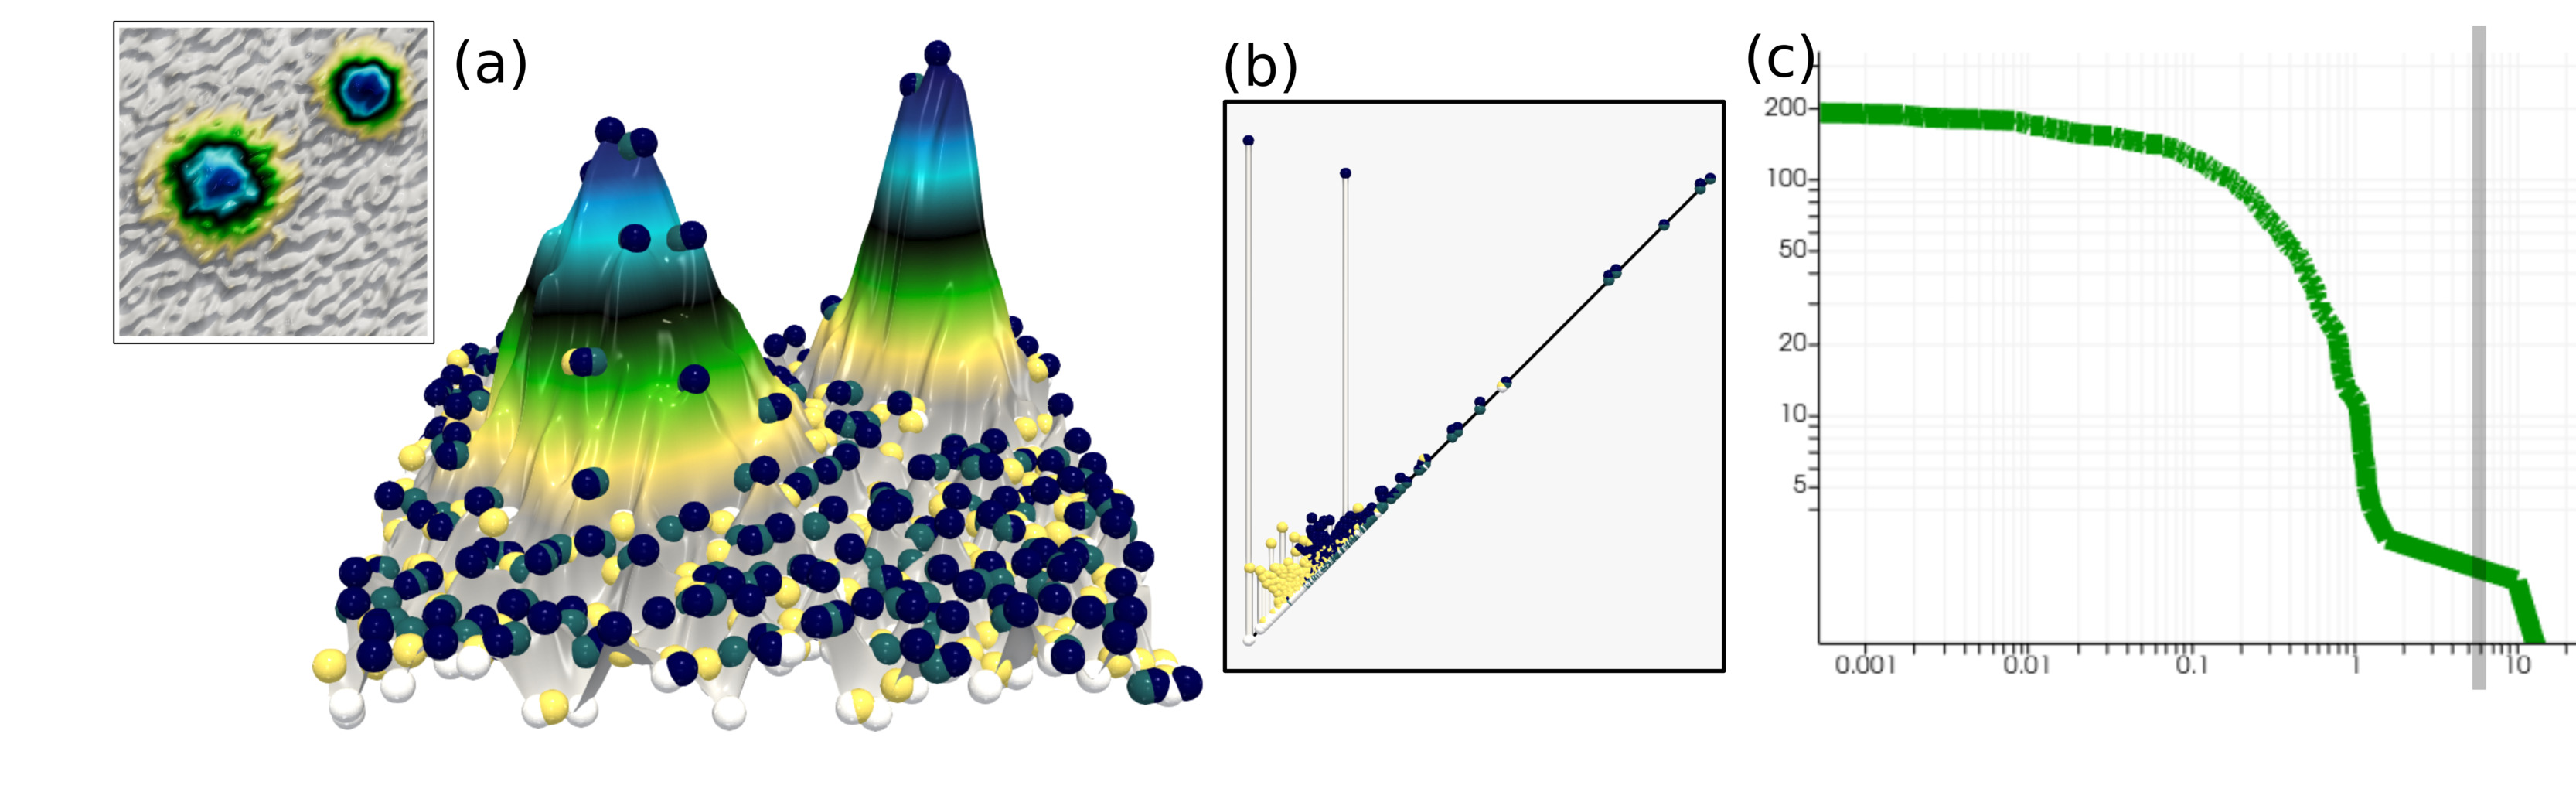
\includegraphics[width=\figureShrink\linewidth]{chapter4_topology_data_analysis/pictures/topo_gaussian.jpg}
 \caption{Critical points (spheres, white: minima, blue: maxima, other:
saddles), persistence diagram (b), persistence curve (c) of
a noisy (a) 2D
scalar field. The persistence diagram captures the main two hills of the
terrain as prominent persistence pairs (large vertical segments), while small
oscillations due to noise induce features near the diagonal.}
 \label{fig_toyTopology}
\end{figure}






\subsection{Topological data analysis}
\label{sec_topology}



This section presents the topological background of our work. It contains
definitions adapted from the Topology ToolKit \cite{ttk17}.
We refer the
reader to textbooks \cite{edelsbrunner09} for an introduction to
% computational
topology.

\noindent
\textbf{Input data.}
The input data is given as an ensemble of $N$ piecewise linear (PL) scalar
fields
$f_i : \domain \rightarrow \range$, with $i \in \{1, \dots,  N\}$, defined on a
PL 2-manifold $\domain$.
Specifically, $f_i$ represents the pointwise flow enstrophy
(\autoref{sec_simulation}) and $\domain$ is the Freudenthal triangulation
\cite{freudenthal42, kuhn60} of a $2$-dimensional regular grid, which is
periodic in both dimensions ($\domain$ is homeomorphic to a $2$-dimensional
torus). The triangulation is performed implicitly, by emulating the
simplicial structure upon traversal queries. Thus it induces no
memory overhead \cite{ttk17}.
The scalar values are given at the vertices of $\domain$ and are linearly
interpolated
on the simplices of higher dimensions.
$f$ is assumed to be injective on the vertices  of $\domain$.
This is
% easily
enforced in practice with a symbolic
perturbation inspired by Simulation of Simplicity \cite{edelsbrunner90}.


\noindent
\textbf{Critical points.}
Topological features in $f_i$ can be tracked with the notion of
\emph{sub-level set}, noted
$\sublevelset{{f_i}}(\isovalue)=\{p \in \domain~|
~f_i(p) < \isovalue\}$. It is defined as the pre-image of  $(-\infty,
\isovalue)$
by
$f_i$.
In particular, the topology of these sub-level sets (in 2D, their connected
components and cycles) can only change at special locations.
As $\isovalue$ continuously increases, the topology of
$\sublevelset{{f_i}}(\isovalue)$ changes at specific vertices of $\domain$,
called the \emph{critical points} of $f_i$ \cite{banchoff70}, defined next.
The \emph{star} of a vertex $v \in \domain$, noted $\Star(v)$,  is
the set of its co-faces:
$\Star(v) = \{ \simplex \in \domain ~|~ v < \sigma \}$.
It can be interpreted as the smallest combinatorial neighborhood around $v$.
The \emph{link} of $v$,
noted $\Link(v)$, is the set of the faces $\face$ of the simplices $\simplex$
of $\Star(v)$ with empty intersection with $v$:
$\Link(v) = \{ \face \in \domain ~ | ~ \face < \simplex, ~
\simplex\in \Star(v), ~ \face \cap v = \emptyset\}$.
The link of a vertex can
be interpreted as the boundary of its star.
The \emph{lower link} of $v$, noted $\lowerlink(v)$, is given by the
set of simplices of $\Link(v)$ which only contain vertices \emph{lower} than
$v$:
$\lowerlink(v) = \{ \simplex \in \Link(v) ~ | ~ \forall v' \in \sigma, ~ f_i(v')
< f_i(v)\}$. The upper link is defined symmetrically: $\upperlink(v) = \{
\simplex \in \Link(v) ~ | ~
\forall v' \in \sigma, ~ f_i(v') > f_i(v)\}$.
A vertex $v$ is \emph{regular}  if
and only if
both $\lowerlink(v)$ and $\upperlink(v)$ are simply connected. For
such vertices, the sub-level sets do not change their topology as they span
$\Star(v)$. Otherwise, $v$ is
a \emph{critical point}.
% of $f$ \cite{banchoff70}.
These can be classified with regard to their
\emph{index} $\Index(v)$.
It is equal to $0$ for local minima
($\lowerlink(v) = \emptyset$), to 2 for local maxima
($\upperlink(v) = \emptyset$) and otherwise to 1 for
saddles (\autoref{fig_toyTopology}a).
In practice, $f_i$ is enforced to contain only isolated, non-degenerate
critical points \cite{edelsbrunner90, edelsbrunner03}.
In the case of
the pointwise flow enstrophy, local maxima denote the center of vortices in the
turbulent flow. However, since the critical point characterization is based on a
classification which is only local (restricted to the link of each vertex), the
slightest oscillation in the data results in practice in the appearance of
spurious critical points, especially in the case of noisy data such as
turbulent flows. This motivates the introduction of an importance measure on
critical points, discussed next, in order to disambiguate vortices from noise.




\noindent
\textbf{Persistence diagrams.}
Several important
measures for critical points have been studied \cite{carr04},
including \emph{topological persistence} \cite{edelsbrunner02}, which is tightly
coupled to the notion of Persistence diagram \cite{edelsbrunner09}, which we
briefly describe here.
Persistence
assesses the importance of a critical point, based on the
lifetime of the topological feature it created (or destroyed) in
 $\sublevelset{{f_i}}(w)$, as one continuously increase the isovalue $w$.
In particular, as $w$ increases, new connected components of
$\sublevelset{{f_i}}(w)$ are created at the minima of $f_i$. The Elder rule
\cite{edelsbrunner09} indicates that if two connected
components, created at the minima $m_0$ and $m_1$ with $f_i(m_0) < f_i(m_1)$,
meet
at a given saddle $s$, the \emph{youngest} of the two components (the
one created at $m_1$) \emph{dies} in favor of the \emph{oldest} one (created at
$m_0$). In this case, a \emph{persistence pair} $(m_1, s)$ is created and
its
\emph{topological persistence} $p$ is given by $p(m_1, s) = f_i(s) - f_i(m_1)$.
All the local minima
can be
unambiguously
paired following this strategy, while the
global minimum is usually paired, by convention, with the global maximum.
The symmetric reasoning
can be applied to characterize, with saddle/maximum pairs, the life
time of the independent cycles of
$\sublevelset{{f_i}}(w)$.
Persistence pairs are usually
visualized with the \emph{Persistence diagram} $\diagram(f_i)$
\cite{edelsbrunner09}, which embeds each pair $(c, c')$, with $f_i(c) <
f_i(c')$,
as a point in the 2D plane, at location $\big(f_i(c), f_i(c')\big)$.
The  value $f_i(c)$ is 
% usually 
called the \emph{birth} of the
feature, while $f_i(c')$ is called its \emph{death}.
The
pair
persistence
can be
visualized as the height of the point to the diagonal.
Features with a high persistence stand out, away from the diagonal,
while noisy features are typically located in its vicinity 
(\autoref{fig_toyTopology}b).
The conciseness, stability \cite{edelsbrunner02} and expressiveness of this
diagram made it a popular tool
for data summarization tasks, as
it provides visual hints about the number, ranges and salience
of the features of interest.
To compare two datasets $f_i$ and $f_j$, persistence diagrams can be efficiently compared with the notion of $L_2$-Wasserstein distance \cite{CohenSteinerEH05,
Turner2014, Kerber2016} (we leave the practical study of distances between more
advanced topological descriptors  \cite{SridharamurthyM20,
pont_vis21} to future work). This distance is based on a bipartite assignment optimization problem (between the points of the two diagrams to compare), for which exact \cite{Munkres1957} and approximate \cite{Bertsekas81}
implementations are publicly available \cite{ttk17, ttk19}.
Specifically, we use in our approach the fast approximation scheme by Vidal et al. \cite{vidal_vis19}.
We refer the reader to \cite{Kerber2016, vidal_vis19, ttk19} for further
% practical
details.
Once the $L_2$-Wasserstein distance between two diagrams $\diagram(f_i)$ and $\diagram(f_j)$ is available (noted $\wasserstein{2}\big(\diagram(f_i), \diagram(f_j)\big)$), more advanced geometrical objects can be considered, such as \emph{Wasserstein barycenters} \cite{Turner2014, vidal_vis19}, which are
% representative
diagrams minimizing the sum of their distance to an ensemble of diagrams, and which consequently, can be considered as a reliable representative of the ensemble.
This notion of \emph{barycenter}
% it
is conducive to the design of clustering algorithms.
% , directly in
% the Wasserstein metric space.
% In particular,
The $k$-means algorithm
% \cite{elkan03, celebi13}
can be easily extended,
by using $\wasserstein{2}$ to measure distances between diagrams, and by
considering as cluster centroid, at each iteration of the $k$-means, the
 barycenter of the cluster.


\noindent
\textbf{Persistence curves.}
A popular, alternate, representation of persistence features is the notion of
\emph{Persistence Curve}, noted $\persistentCurve(f_i)$, which plots the
population of persistent pairs as a function of their persistence.
Specifically, it encodes the number of pairs (Y axis) whose persistence is
\emph{larger} than a threshold $\epsilon$ (X axis).
For $X=0$, $Y$ is equal to the total number of persistence pairs, while for the
largest values of $X$, $Y$ indicates the number of prominent, high-persistence
features (\autoref{fig_toyTopology}c).
In practice, large
plateaus in this curve will indicate \emph{stable} persistence ranges, for
which no (or few) topological features are present in the data. These 
correspond to \emph{separations} (vertical line, \autoref{fig_toyTopology}c) 
between populations of topological
features of distinct persistence scales, typically the noise (low $X$
values) and the persistent features (high $X$ values).





\section{Background}
\label{sec_background}
This section presents the background used in this study in $(i)$ numerical simulation by presenting the equations, the interpolation schemes and the solvers implemented in our simulation code. Then the background in $(ii)$ topological data analysis introduces the main notions used such as critical points, persistence diagrams or the Wasserstein distant metric.

\subsection{Numerical simulation}
\label{sec_simulation}
\label{sec_solvers}

In this work, we consider the two-dimensional compressible unsteady Euler equations for inviscid flows \cite{masatsuka2013}:
% which
% are solved.
% The system
% can be written as \cite{masatsuka2013}:
\eqSpace
\begin{equation}
    \mathbf{U}_t + \mathbf{F}_x + \mathbf{G}_y = 0,
    \label{eq:cons_euler}
    \eqSpace
\end{equation}
\noindent where the subscripts indicate differentiation, $\mathbf{U}$ is the 
vector of conservative dimensionless variables and $\mathbf{F}$ and $\mathbf{G}$ 
represent the inviscid fluxes in $x$ and $y$ direction respectively.
Those vectors are defined as:
% follow:
\eqSpace
\eqSpace
\eqSpace
\begin{equation}
% \eqSpace
    \begin{array}{l}
        \mathbf{U} = \left[\begin{array}{c}\rho \\ \rho u \\ \rho v \\ \rho E\end{array}\right], ~~
        \mathbf{F} = \left[\begin{array}{c}\rho u \\ \rho u^2 + p\\ \rho u v\\ (\rho E + p)u\end{array}\right], ~~
        \mathbf{G} = \left[\begin{array}{c}\rho v \\ \rho u v \\ \rho v^2 + p \\ (\rho E + p)v\end{array}\right].
    \end{array}
    \label{eq:cons_euler_vectors}
    \eqSpace
\end{equation}
\noindent In the above expressions, $t$ denotes the time and $x$ and $y$ are the Cartesian coordinates.
$\rho$ denotes density, $u$ and $v$ denote the $x-$ and $y-$
coordinates of the velocity vector $\mathbf{w}$,
% direction velocity components, 
$E$ denotes the specific total energy and $p$ denotes the static pressure.
The aforementioned mathematical model is described as it is implemented in the in-house code HYPERION (HYPERsonic vehicle design with Immersed bOuNdaries) whose primary capabilities as a massively parallel structured solver using immersed boundary conditions have already been discussed by Bridel-Bertomeu \cite{bridel2021immersed}.
The present study uses only regular Cartesian grids with constant grid spacings (grid of pixels) in both directions of space, $\Delta x$ and $\Delta y$, and will not rely on any immersed boundary condition during the computations presented later.
This being said, the finite-volume method \cite{leveque2002finite,trangenstein2007numerical,toro2013riemann} is then employed for space discretization of the compressible Euler equations~\eqref{eq:cons_euler}.

The 2D turbulence investigated in our work
% at the heart of this study
is generated using a Kelvin-Helmholtz instability (see \cite{san2015evaluation} for a complete description)
% of the initialization)
simulated with high-order low-dissipation  reconstruction schemes of $5^{\text{th}}$- and $7^{\text{th}}$-order (\autoref{tab_parameters}).
The numerical fluxes between the cells are obtained using a variety of Riemann solvers detail at the end of this section.
To emulate turbulence in a infinite medium, all boundary conditions are set as periodic.
One common measure of turbulence in two dimensions that we will rely on is the 
local enstrophy $\mathcal{E}$, defined locally as the square of the flow vorticity:
% $\mathbf{w}$:
% , \emph{i.e:}
\eqSpace
\begin{equation}
% \eqSpace
    \mathcal{E} = 0.5\left\vert\nabla\times\mathbf{w}\right\vert^2.
    \label{eq:enstrophy}
    \eqSpace
\end{equation}



When solving numerically the Euler equations  (\autoref{eq:cons_euler}), we 
start by interpolating the values of the flows at the cell interfaces.
Then, we have
% We then have
to use an approximate Riemann solver
\cite{toro2013riemann}
to solve the eponymous problem 
on those interfaces.
% In the remaining of this section 
In the remainder,
we will expose the different
% numerical
methods used to make these two
calculations.

\noindent
\textbf{Interpolation schemes.} 
\label{sec_interpolations}
One problem in numerically solving the schemes is to be able to capture the strong discontinuities while capturing the small scales of the turbulence. In addition, we want to be as accurate as possible in our interpolation. To do this, researchers and engineers have developed several high-order reconstruction methods. A common scheme for solving compressible flows in the presence of strong discontinuities is the \textit{Weighted Essentially Non-Oscillatory (WENO)} scheme \cite{liu1994weighted}. Several variants of this scheme have been
introduced,
% made during the last decades,
to improve its performances\cite{jiang1996efficient}\cite{hu2010adaptive}\cite{henrick2005mapped}.
We are particularly interested in two families: the well-known robust but dissipative WENO-Z \cite{borges2008improved} and the TENO (T for \emph{Targeted}) \cite{fu2016family}, which better discriminates scales \cite{hu2011scale}.
% able to better discriminate between scales \cite{hu2011scale}.
% We are particularly interested in the WENO-Z \cite{borges2008improved} scheme, commonly used in the literature and able to keep its theoretical order even when solving for nonlinear systems.
% Unfortunately this scheme is too dissipative and dampens considerably the small scales of the turbulence \cite{zhao2014comparison}\cite{martin2000shock}.
% A second family of interest is that of the \textit{The Targeted Essentially Non-Oscillatory (TENO)} schemes developed by Liu and al \cite{fu2016family} is a high order scheme that attempts to capture turbulence better than WENO-Z while capturing strong discontinuities (shocks).
% It uses new ingredients such as a better discrimination between strong discontinuities and small scale turbulence \cite{hu2011scale}.
%Thus in our simulations, we should see a different number of structures between our two methods.

\noindent
\textbf{Solvers.}
We have to solve the Riemann problems at the interfaces between the cells of the mesh.
One solution is to use an exact Godunov solver \cite{toro2013riemann} which takes into account a large number of nonlinear operations - too expensive however when calculating complex flows. 
Rather, researchers and engineers are interested in approximate Riemann solvers. The most used approximate solvers can be grouped in three large families: Flux Difference Splitting (FDS), Flux Vector Splitting (FVS) and Flux Type Splitting (FTS) \cite{toro2013riemann}.
In this section we will focus on two types of solvers in particular, Flux Difference Splitting solvers that work as a finite volume method to solve the Riemann problem and Flux Splitting Riemann solvers that combine the qualities of the other two families by separating kinematic and acoustic scales.
% This type of solvers capture the strong discontinuities (shock), and calculate accurately the boundary layers.

\noindent
\textbf{HLL} \textit{(Harten, Lax, and van Leer)} : FDS
% type
scheme developed by
Harten et al. \cite{harten1983upstream}.
% This scheme
It does not take into account
contact discontinuities, i.e. lines crossing two states.
% (slip line).
% In the study of turbulent phenomena,
For turbulent phenomena,
the interface between vortices will
therefore be less described.

\noindent
\textbf{Roe}  and \textbf{HLLC} \textit{(Harten, Lax, and van Leer with Contact)} : FDS type schemes developed by \cite{toro1994restoration}\cite{Roe1981approximate}. These two schemes are robust and thus allow to reproduce the strong discontinuity (shock) and takes into account the discontinuities of contact. Thus, with these schemes, the reconstruction of the vortices represented in our flows, is perform with more accuracy than with the HLL solver.

\noindent
In its study on low speed Riemann solvers, \cite{qu2014study} notice that the solvers are unable to obtain physical solutions. Therefore, there is a need for approximate Riemann solvers to accurately reconstruct both low and high speed flows. This is why we are interested in two flux type splitting (FTS) solvers, which take into account all velocities to obtain low Mach and high Mach physics solutions.

\noindent
\textbf{AUSM$^+$-UP} \textit{(Advection Upstream Splitting Method +UP)} : By adding improvements \cite{liou2006sequel} to the AUSM+ \cite{liou1996sequel} solver Liou increases its level of accuracy for all speeds. This new solver takes into account contact discontinuities, reconstructs also strong discontinuities and gives physical solutions for all speeds.

\noindent
\textbf{SLAU2} \textit{(Simple Low-Dissipation AUSM 2)} :
% the study conducted on
the analysis of the dissipation pressure term of the AUSM+ \cite{shima2009new} shows that it is too high for low speeds.  The author decided to control the pressure flux and implemented the SLAU solver.
This
% work
has been extended
\cite{kitamura2013towards}
% extends the work on this term
so that the dissipation becomes proportional to the Mach number. This solver takes into account contact discontinuities, reconstructs also strong discontinuities and gives physical solutions for all speeds.







\section{Case Study}

\label{sec_caseStudy}
In this section, we give \emph{(i)} a description of the ensemble (made publicly
available \cite{data})
% data
representing the Kelvin Helmholtz Instabilities (KHI) computed on 
%the CEA 
our institution's
facilities.
% which has 
% been 
% .
Next, we state \emph{(ii)} the challenges in understanding
such phenomena and we
% edict
provide
\emph{(iii)} theoretical hypothesis that our
experimental protocols have to verify.   

\begin{figure}
 \centering
 \vspace{-1ex}
 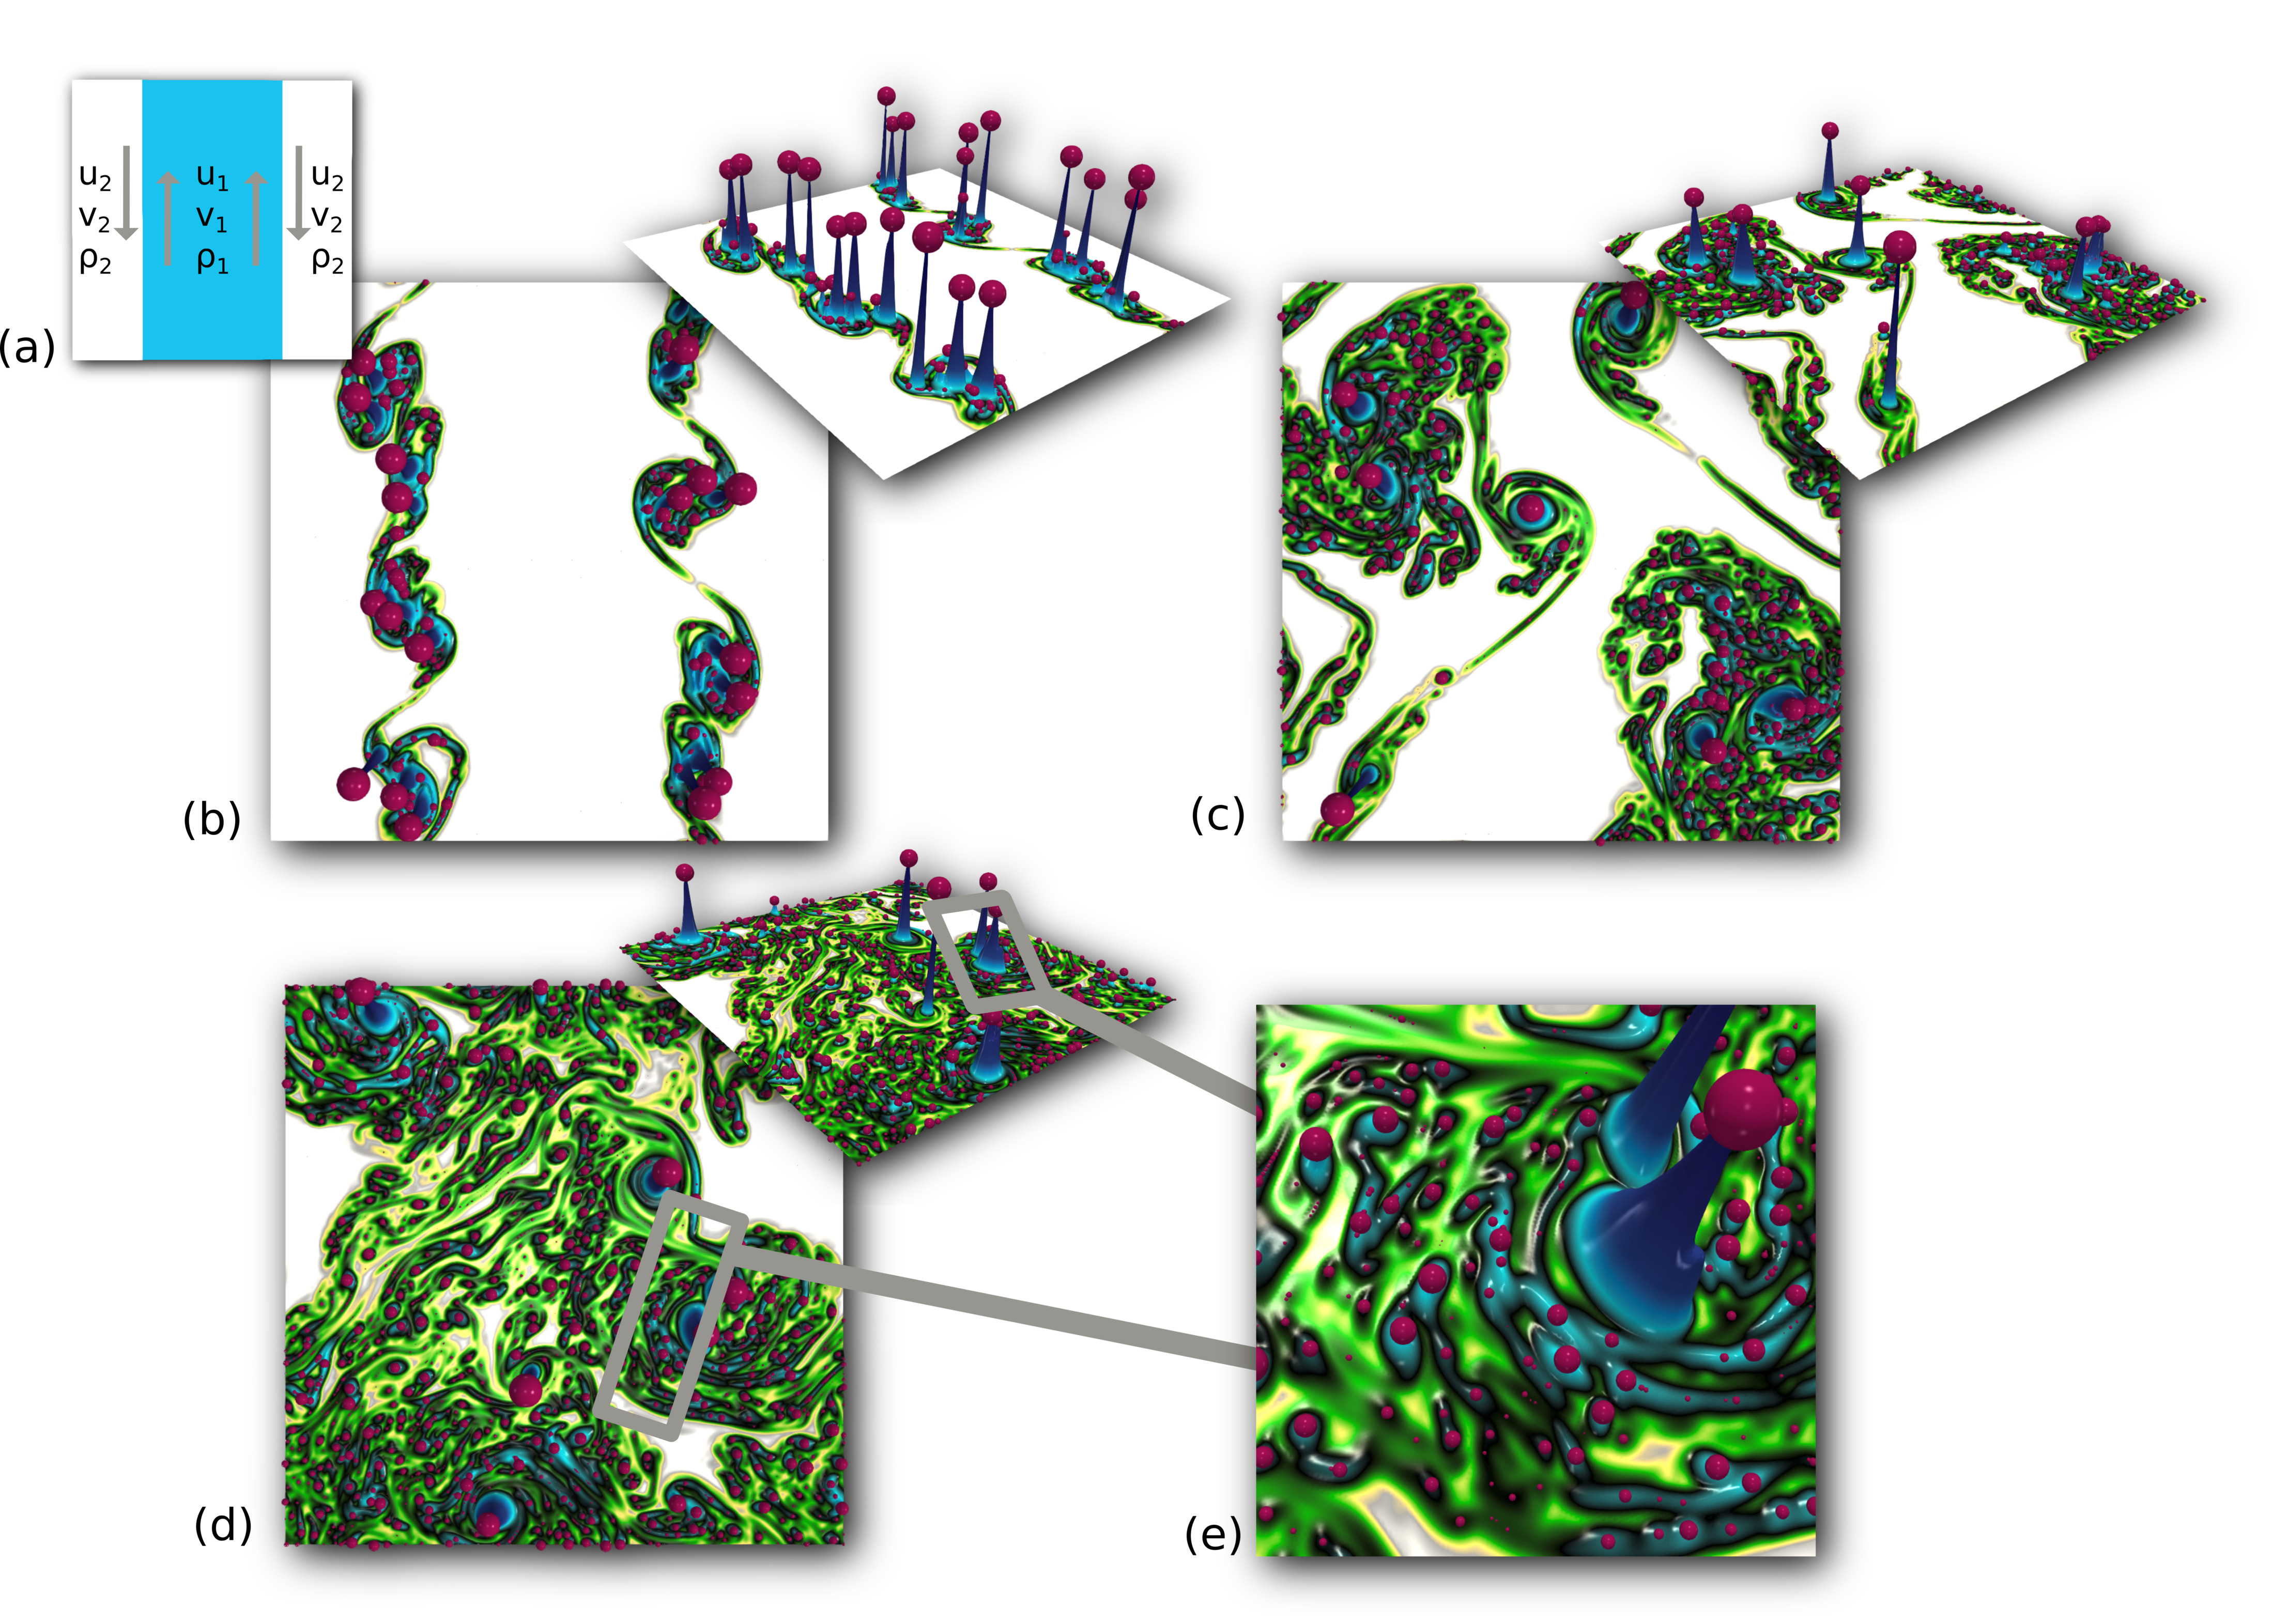
\includegraphics[width=\figureShrink\linewidth]{chapter4_topology_data_analysis/pictures/init_case.jpg}
 \vspace{-2ex}
 \mycaption{Initialization of the Kelvin-Helmholtz instability (a). This simulation was obtained
with the AUSM$^+$-UP solver with a TENO 5 order interpolation at physical times $0.25$(b), 
$0.75$(c) and $1.25$(d). Red spheres scaled by the persistence represent the maximum critical points. Zoom of the turbulence structures (e).}
  \vspace{2ex}
 \label{initcase}
\end{figure}

\subsection{Data description}
The initialization of the KHI was generated with two fluids of different 
densities ($\rho_{1}$, $\rho_{2}$) (\autoref{initcase}a). The
different velocities of opposite direction ($\{u _{1},v_{1}\},\{u _{2},v_{2}\}$) 
of the fluids create a shearing zone where the turbulence appears with the KHI 
(\autoref{initcase}b). While the instability develops over time the main 
vortices grow (\autoref{initcase}c). After a longer simulation time, the main 
structures keep evolving (\autoref{initcase}d) and a large number of 
small-scale vortices appear in the vicinity of large-scale vortices
% around the main structures 
(\autoref{initcase}e) 
leading to a complex turbulent flow. This variation in vortex scale,
% of the
% vortices,
in addition to the chaotic flow geometry,
% of the flow,
is notoriously
challenging for the analysis of turbulent flows.

\begin{table}
\centering
\scalebox{0.8}{
\begin{tabular}{|c|c|c|c|c|c|c|}
\hline
Parameter            & Resolution           & Order                &  Time       
       &  Solver              &  Scheme              &  Total              \\ 
\hline
\hline
                     &                      &                      &             
         &  HLL            &                 &                \\
                     &  256                 &      5               &       t$_0$ 
         &  SLAU2          &  TENO         &                \\
Value                &  512                 &      7               &       t$_1$ 
         &  AUSM$^+$-UP         &  WENO-Z        &                \\
                     &  1024                &                      &       t$_2$ 
         &  Roe            &                &                \\
                     &                      &                      &             
         &  HLLC           &                &                \\                  
                                             
\hline
\hline
Number&3&2&3&5&2&180\\
\hline
\multicolumn{1}{l}{} & \multicolumn{1}{l}{} & \multicolumn{1}{l}{} & 
\multicolumn{1}{l}{} & \multicolumn{1}{l}{} & \multicolumn{1}{l}{} & 
\multicolumn{1}{l}{} 
\end{tabular}
}

\caption{Parameter space of the HYPERION simulation code leading to a total of 180 members for the ensemble dataset used in this study.}
\vspace{-3ex}
\label{tab_parameters}
\end{table}

% This is why, in the section 
% \autoref{sec_experimentalResults} we study how the topological analysis of the 
% % enstrophy can capture features in the KHI and thus help us to compare them. 

The HYPERION simulation code introduced in \autoref{sec_simulation} has been 
used to generate the ensemble dataset. All the simulations have been run on a 
supercomputer 
% of the CEA 
at our institution. Each simulation have been executed in parallel using 16 MPI processes and have been distributed over the supercomputer. The total 
simulation took about 745 CPU hours. The raw data has been dump on disk with the 
metadata stored in XDMF files and the scalar fields in HDF5 files leading to 14 
GB for the entire ensemble dataset. We processed these results to extract the 
enstrophy scalar field (\autoref{eq:enstrophy}) and stored it to a VTK file 
format \cite{Kitware:2003} using an image data structure for regular grids 
(VTI). This reduces the entire ensemble to 600 MB. 

The ensemble dataset corresponds to different computational configurations for 
the same turbulent instability. HYPERION handles different parameter types such 
as scalars or enumerations, which allows the users to compute various numerical 
simulations in the same parametric study. The resolution of the 2D regular grid, 
the simulation time, the interpolation scheme, the order of interpolation and 
the Riemann solvers presented in \autoref{sec_background} are our different 
parameters. \autoref{tab_parameters} details the parameter types and values as 
well as the number of samples per parameter, leading overall to an ensemble of 
$3\times2\times3\times5\times2=180$ members illustrated \autoref{fig_teaser}a. 
Each parameter value of \autoref{tab_parameters} used to run the simulation has 
been stored as meta-data in the VTI files (i.e. \emph{Field Data} in the VTK 
terminology)  to keep track of the computational configuration for later 
analysis down the pipeline.
In order to ease the exploration of the ensemble dataset, we defined a 
SQL-type database using the cinema database feature of TTK \cite{ttk17, ttk19}. 
This representation facilitates the extraction of sub-samples of the ensemble, 
based on standard SQL queries on the simulation parameters 
(\autoref{tab_parameters}).

% This database eases the query to extract sub-samples of the ensemble using the 
% input parameters referenced in \autoref{tab_parameters}.\julien{référencer 
% l'annexe pour le détail technique des temps ?}



\begin{figure}
 \centering
 \vspace{-1ex}
 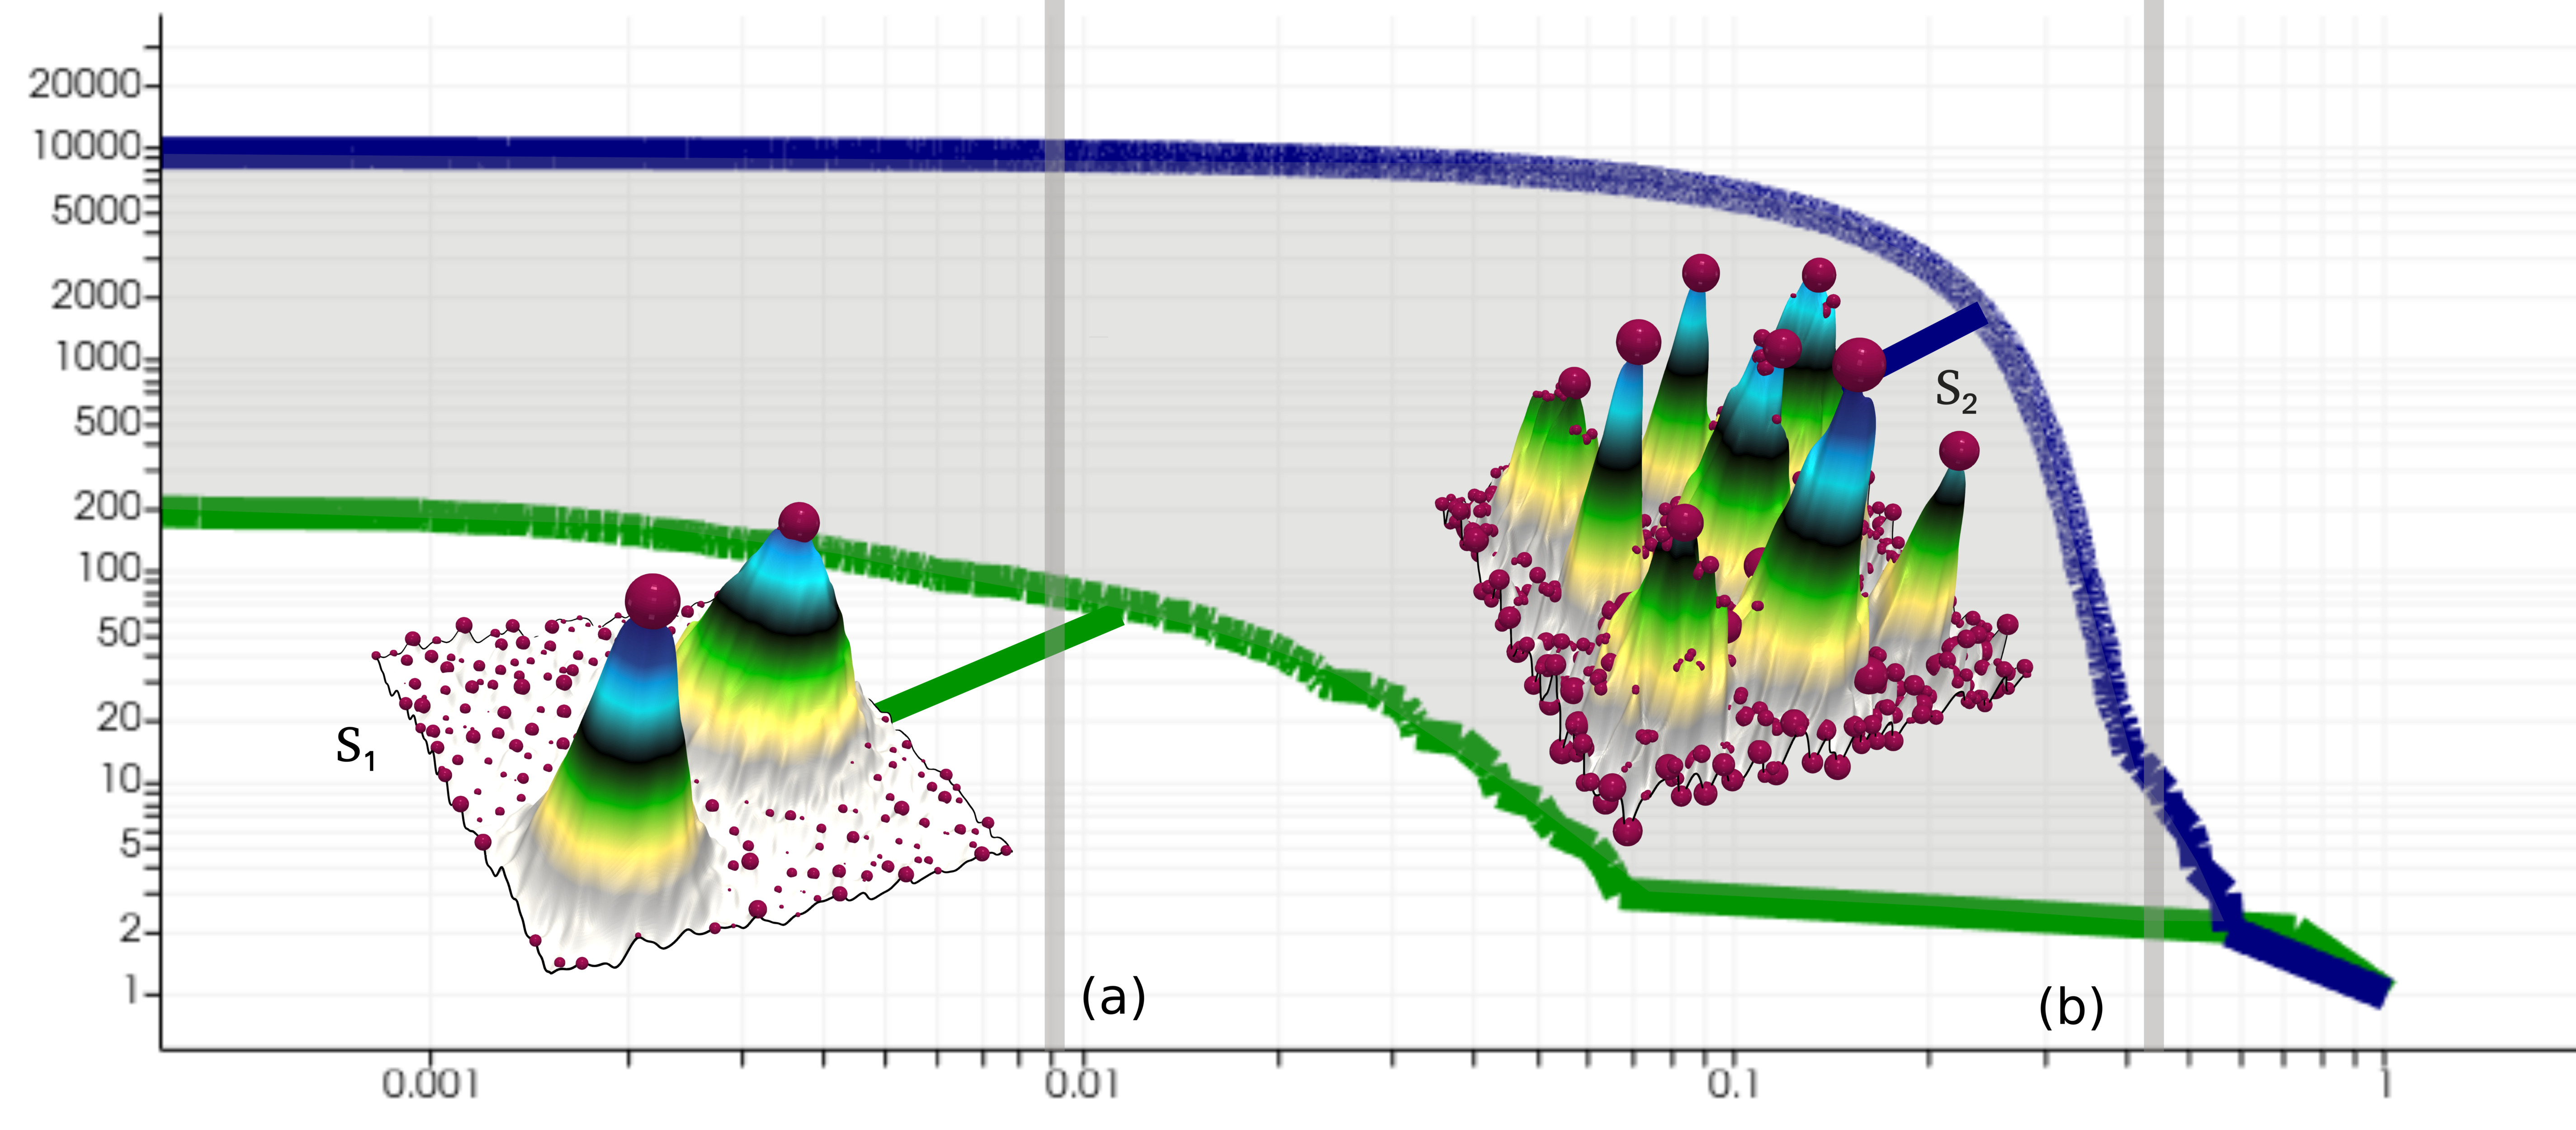
\includegraphics[width=\figureShrink\linewidth]{chapter4_topology_data_analysis/pictures/gaussian_courbe.jpg}
 \mycaption{Persistence curves for two input scalar fields (X-axis: persistence threshold, Y-axis: number of maxima more persistent than X). $S_1$ generated with two Gaussian functions with noise and $S_2$ with 10 Gaussian functions with a stronger noise. Maxima critical points are represented by red spheres scaled by persistence. Vertical line corresponds to
 (a) small persistence critical points, (b) to high persistence. The grey area is the integral difference between the two curves.}
 \label{fig_gaussian_curve}
\end{figure}

\subsection{Problem statement}

% For numerical computation in fluid dynamics there are several methods of interpolation and Riemann solvers.
% For today's engineers who design vehicles it is important to use accurate methods to recover for example heat fluxes, pressure at the walls to be able to dimension correctly their future vehicles.
% Nevertheless, it is also necessary to take into account the calculation time which can be extremely high, especially with 3-dimensional calculations.
% The calculation of the turbulence is then important because this phenomenon will bring fluctuations of the data that we analyze and it is then necessary to capture it with precisions too.
% It is a fractal phenomenon that we analyze by averaging on the domain a value to look at scpectra later.
% With this traditional treatment it is difficult to see a real difference between the numerical methods and especially for the solvers.
% That's why we want to use the topology to maybe guide our choice of numerical methods.
% -- 
Vehicle design, be it in an automotive or aeronautical context, is well known for its high number of constraints that are nowadays most often handled with the help of computational techniques.
In the aeronautical world for instance, engineers today face an incredible challenge wherein they have to be able to predict, at the same time, integral quantities at the wall of the vehicle such as heat flux or pressure as well as three-dimensional phenomena such as flow discontinuities and turbulence.
In other words, engineers have to deal with multiple types of physics and phenomena that have markedly different length- and time-scales but whose interactions are still of great importance to the accuracy of their predictions.
With limited time and resources to conduct the computer-aided simulations, the traditional approach is to rely on numerical strategies that temporally average most of the three-dimensional phenomena and rely more or less on models of turbulence to yield a fast and reasonable forecast.

Even in such a context of approximate simulations, the choice of the ingredients of the numerical recipe matters - methods of reconstruction, Riemann solvers, etc.
Making the right choices can indeed bring a significant increase in fidelity to the engineer, especially in terms of turbulence, by lessening the need for modeling and henceforth bring more margin in the design of the vehicle.
Turbulence is however by nature a chaotic phenomenon and conducting a systematical study of the impact of the different
% aforementioned
numerical ingredients thereupon might prove tricky for a simple reason: beyond a certain level of accuracy, everything will \emph{look} the same.
Detecting the benefits of one method compared to another in that situation will be next to impossible - that is, with traditional techniques.
We propose here to use the ability of topological analysis to discern features that stay otherwise hidden in traditional fluid dynamics postprocessing to help with the choice of the right numerical ingredients. 



\subsection{CFD Hypotheses}
\label{sec_hypotheses}
This section introduces the hypotheses provided by CFD experts, documenting their expectations about ensemble flow variability.
% in the ensemble.}

% \florent{Here are the assumptions considered in this study, provided by CFD experts, with a literature search.}

\label{Hypotheses}
\noindent
\textbf{Hypothesis H1.}
% It is assumed that
TENO induces more turbulence (i.e. more critical points) than
% the
WENO-Z, for all configurations.\\
% no matter the resolution, the time or the solver is.\\
\textbf{Hypothesis H2.}
Order 5 and 7 are equivalent for Kelvin Helmholtz instabilities.\\
% In the literature, studies have been conducted on turbulence and notably on Kelvin Helmholtz to show that orders 5 and 7 are equivalent. We therefore try to find an independence of the orders using our topological analysis.\\
\textbf{Hypothesis H3.}
The HLL solver should provide a significantly distinct description, for all configurations.\\
% It is assumed that the HLL solver describes very differently the instabilities for all resolutions and schemes. It's a dissipative solver and doesn't take into account the dissipative
% contact discontinuities.\\
\textbf{Hypothesis H4.}
The HLLC and Roe solvers should provide equivalent outputs for all configurations.\\
% (and should therefore belong to the same cluster).\\
% It is assumed that HLLC and Roe are in the same cluster for all resolutions and schemes. These solvers are of FDS type, they take into account the contact discontinuities, but do not adapt to all Mach.\\
\textbf{Hypothesis H5.}
The
% It is assumed that
SLAU2 and AUSM$^+$-UP solvers should provide equivalent outputs for all configurations.\\
% are in the same cluster for all resolutions and schemes.
% They are FTS type solvers, they have the characteristics of being not very dissipative and they adapt to all speeds.\\

The above hypotheses are direct consequences of
% prior experimental
observations, or
% solver
design choices. For instance, the TENO scheme has been reported to capture turbulence more accurately \cite{peng2021efficient}, which is expressed by Hypothesis H1. Similar kinetic energy curves (\autoref{energie}) have been reported for the orders 5 and 7, which is expressed by Hypothesis H2. The HLL solver, which is a dissipative approach, is known to model contact discontinuities poorly in contrast to more recent solvers, which is expressed in Hypothesis H3 \cite{toro2013riemann}. Finally, unlike the SLAU2 and AUSMUP (FTS type) solvers, the HLLC and RoE (FDS type) solvers have been reported to provide unphysical results at both low and high velocities (resulting in local oscillations in pressure and density), which is expressed in Hypotheses H4 and H5. %\cite{qu2021review}.

From a practical point of view, the validation of these hypotheses has a major impact for the engineers when setting up their simulations. For instance, the validation of the Hypothesis H1 would justify the usage of a more computationally expensive scheme (TENO), while the validation of the Hypothesis H2 would enable the usage of less computationally expensive orders (5 instead of 7). Finally, the validation of the Hypotheses H3, H4, and H5 would help engineers properly select the most appropriate solvers, based on their flow characteristics.
% expected velocities.
Then, overall, the validation of these hypotheses
% is important towards the
would provide reliable rules-of-thumb for the tuning of the solvers,
% enables more confidence when
% proper
% tuning of the solvers,
to achieve the best balance between accuracy and speed.

% \florent{Referring to the publication of liu fu,(Add ref \cite{peng2021efficient}) who developed the TENO scheme, and who compared it to the weno scheme on several test cases, the TENO has the ability to capture with more accuracy the turbulence phenomenon.  By looking at the topological approaches to the results obtained between these two schemes we should observe differences in the number of structures that are reconstructed(H1).}
% \florent{A study on weno(ref) schemes, using a KHI as a test case, shows that for order 5 and 7, a similar result is obtained on the kinetic energy curves (\autoref{energie}).}
% \florent{Assumptions H4 and H5 allow us to compare Riemann solvers that do or do not calculate all velocities in a numerical simulation. According to the literature (add ref). The HLLC and ROE solvers fail to calculate both high and low velocities, which leads to small oscillations (pressure or density) in the simulation results, unlike the SLAU2 and AUSMUP solvers.
% Validating the Hypotheses will help engineers to choose which tools to use to set up their numerical simulations by minimising the computational cost and to gain precision in the numerical methods used.}




\subsection{Baseline analysis}
Traditional approaches for turbulent data analysis (\autoref{energie}) are based on an average of
quantities of interest, such as flow energy (\autoref{sec_relatedWork}).
The $L_2$ norm is another established distance for comparing scalar fields. Both strategies bear similarities in their averaging artifacts: they cannot distinguish the contribution
of small structures from the global flow, because these are masked by the weight
of larger vortices.
%
% However, this average strategy
% % the energy or the enstrophy (see
% % \autoref{sec_relatedWork} and \autoref{energie}).
% such an averaging is similar to the averaging
% effect of the $L_2$-norm, when used for comparing enstrophy fields.
% % These averages correspond to the calculation of $L_2$-distances between the
% % solutions.
% In particular, this distance does not allow to see the contribution
% of the small structures to the global flow because they are masked by the weight
% of larger structures.
Moreover, the $L_2$-norm is also very sensitive to mild geometric variations,
whereas the chaotic nature of turbulent flows induces major geometric
variations between ensemble members.
This motivates the usage of  topological methods to capture
features in the KHI that will help us compare the members
(\autoref{sec_experimentalResults}). In the remainder, we will systematically compare our protocols based on topological distances (\autoref{sec_protocols}) to the $L_2$ norm, considered as the baseline approach, and detailed comparisons will be provided (\autoref{sec_experimentalResults}).




\section{Evaluation protocols}
\label{sec_protocols}
In this section, we present 3 protocols which can be used to verify the
hypotheses detailed in \autoref{Hypotheses}. One can directly use these
algorithms on the ensemble dataset. It corresponds to $(i)$ the separation of
the schemes and the independence of the orders, $(ii)$ the unique behavior of
the HLL solver and $(iii)$ similarities in class of solvers.


\subsection{Persistence curves}
\label{sec_persistence}
With this protocol (illustrated on toy examples, \autoref{fig_gaussian_curve}), we want to validate hypothesis H1 (\autoref{Hypotheses}) to discriminate the interpolation schemes TENO and WENO-Z regarding the differences in the enstrophy field. With this protocol, we also want to validate hypothesis H2 (\autoref{Hypotheses}) to confirm the independence of the orders \cite{san2015evaluation}. To better characterize the vortices influencing the turbulence, we use persistence curves (\autoref{sec_topology}). These curves will
allow us to threshold the structures (the eddies) at different scales and
thus to easily compare the number of small (\autoref{fig_gaussian_curve}a) and large (\autoref{fig_gaussian_curve}b) eddies using the integral of the persistence curve.

For the differentiation of the schemes, we take 5 simulation configurations where the physical time ($t_0,t_1,t_2$), the resolution ($256\times 256$, $512\times 512$, $ 1024\times 1024$) and the order (5,7) are fixed per sample (\autoref{tab_parameters}). The variation is the interpolation scheme (TENO, WENO-Z). For the order independence, 5 configurations are also chosen by fixing the physical time ($t_0,t_1,t_2$), the resolution ($256\times 256$, $512\times 512$, $ 1024\times 1024$), the scheme (TENO or WENO-Z). The variation is done on the order (5,7). Besides different input variations,
% to build the configurations,
this protocol is the same for testing H1 and H2.

The persistence curves are generated for all the samples. Then, we average the 5 persistence curves (one per solver) to obtain 2 average persistence curves with respect to the variable parameters (schemes or orders). Finally, we compute the difference of the integrals between the two averaged curves (grey area on \autoref{fig_gaussian_curve}). The small values on the curves under a persistence of $10^{-6}$ correspond to numerical noise coming from the different simulation steps. They are removed from the computation of the integral with a threshold at $10^{-6}$(\autoref{fig_gaussian_curve}.a). The integral curve difference corresponds to our metric allowing to precisely describe the similarity in the topology of the critical points. Bigger is the integral, the more different the topology of the flow is. Thus, to verify hypothesis H1 related to the scheme, we want the difference of the integrals to be high. To verify hypothesis H2 related to the orders, we want the difference of the integrals to be close to zero.


\begin{figure}
 \centering
 \vspace{-1ex}
 
\includegraphics[width=\figureShrink\linewidth]{chapter4_topology_data_analysis/pictures/gaussian_distance_to_the_rest.jpg}
 \mycaption{
 Wasserstein distance matrix for five inputs $S_1$, $S_2$, $S_3$,$S_4$, $S_5$
 generated respectively with two, five, four and three Gaussians
%  functions
 with varying noise.
% different noise levels.
The sum of each
matrix line
% line of the matrix
is
% computed and
normalized with respect to the scalar-field that maximizes the distances, here
$S_1$. We see that $S_1$ with only two Gaussians is very far from the other
datasets.}
 \label{gaussian_distance}
\end{figure}
\begin{figure}
\vspace{-1ex}
 \centering % avoid the use of \begin{center}...\end{center} and use \centering
 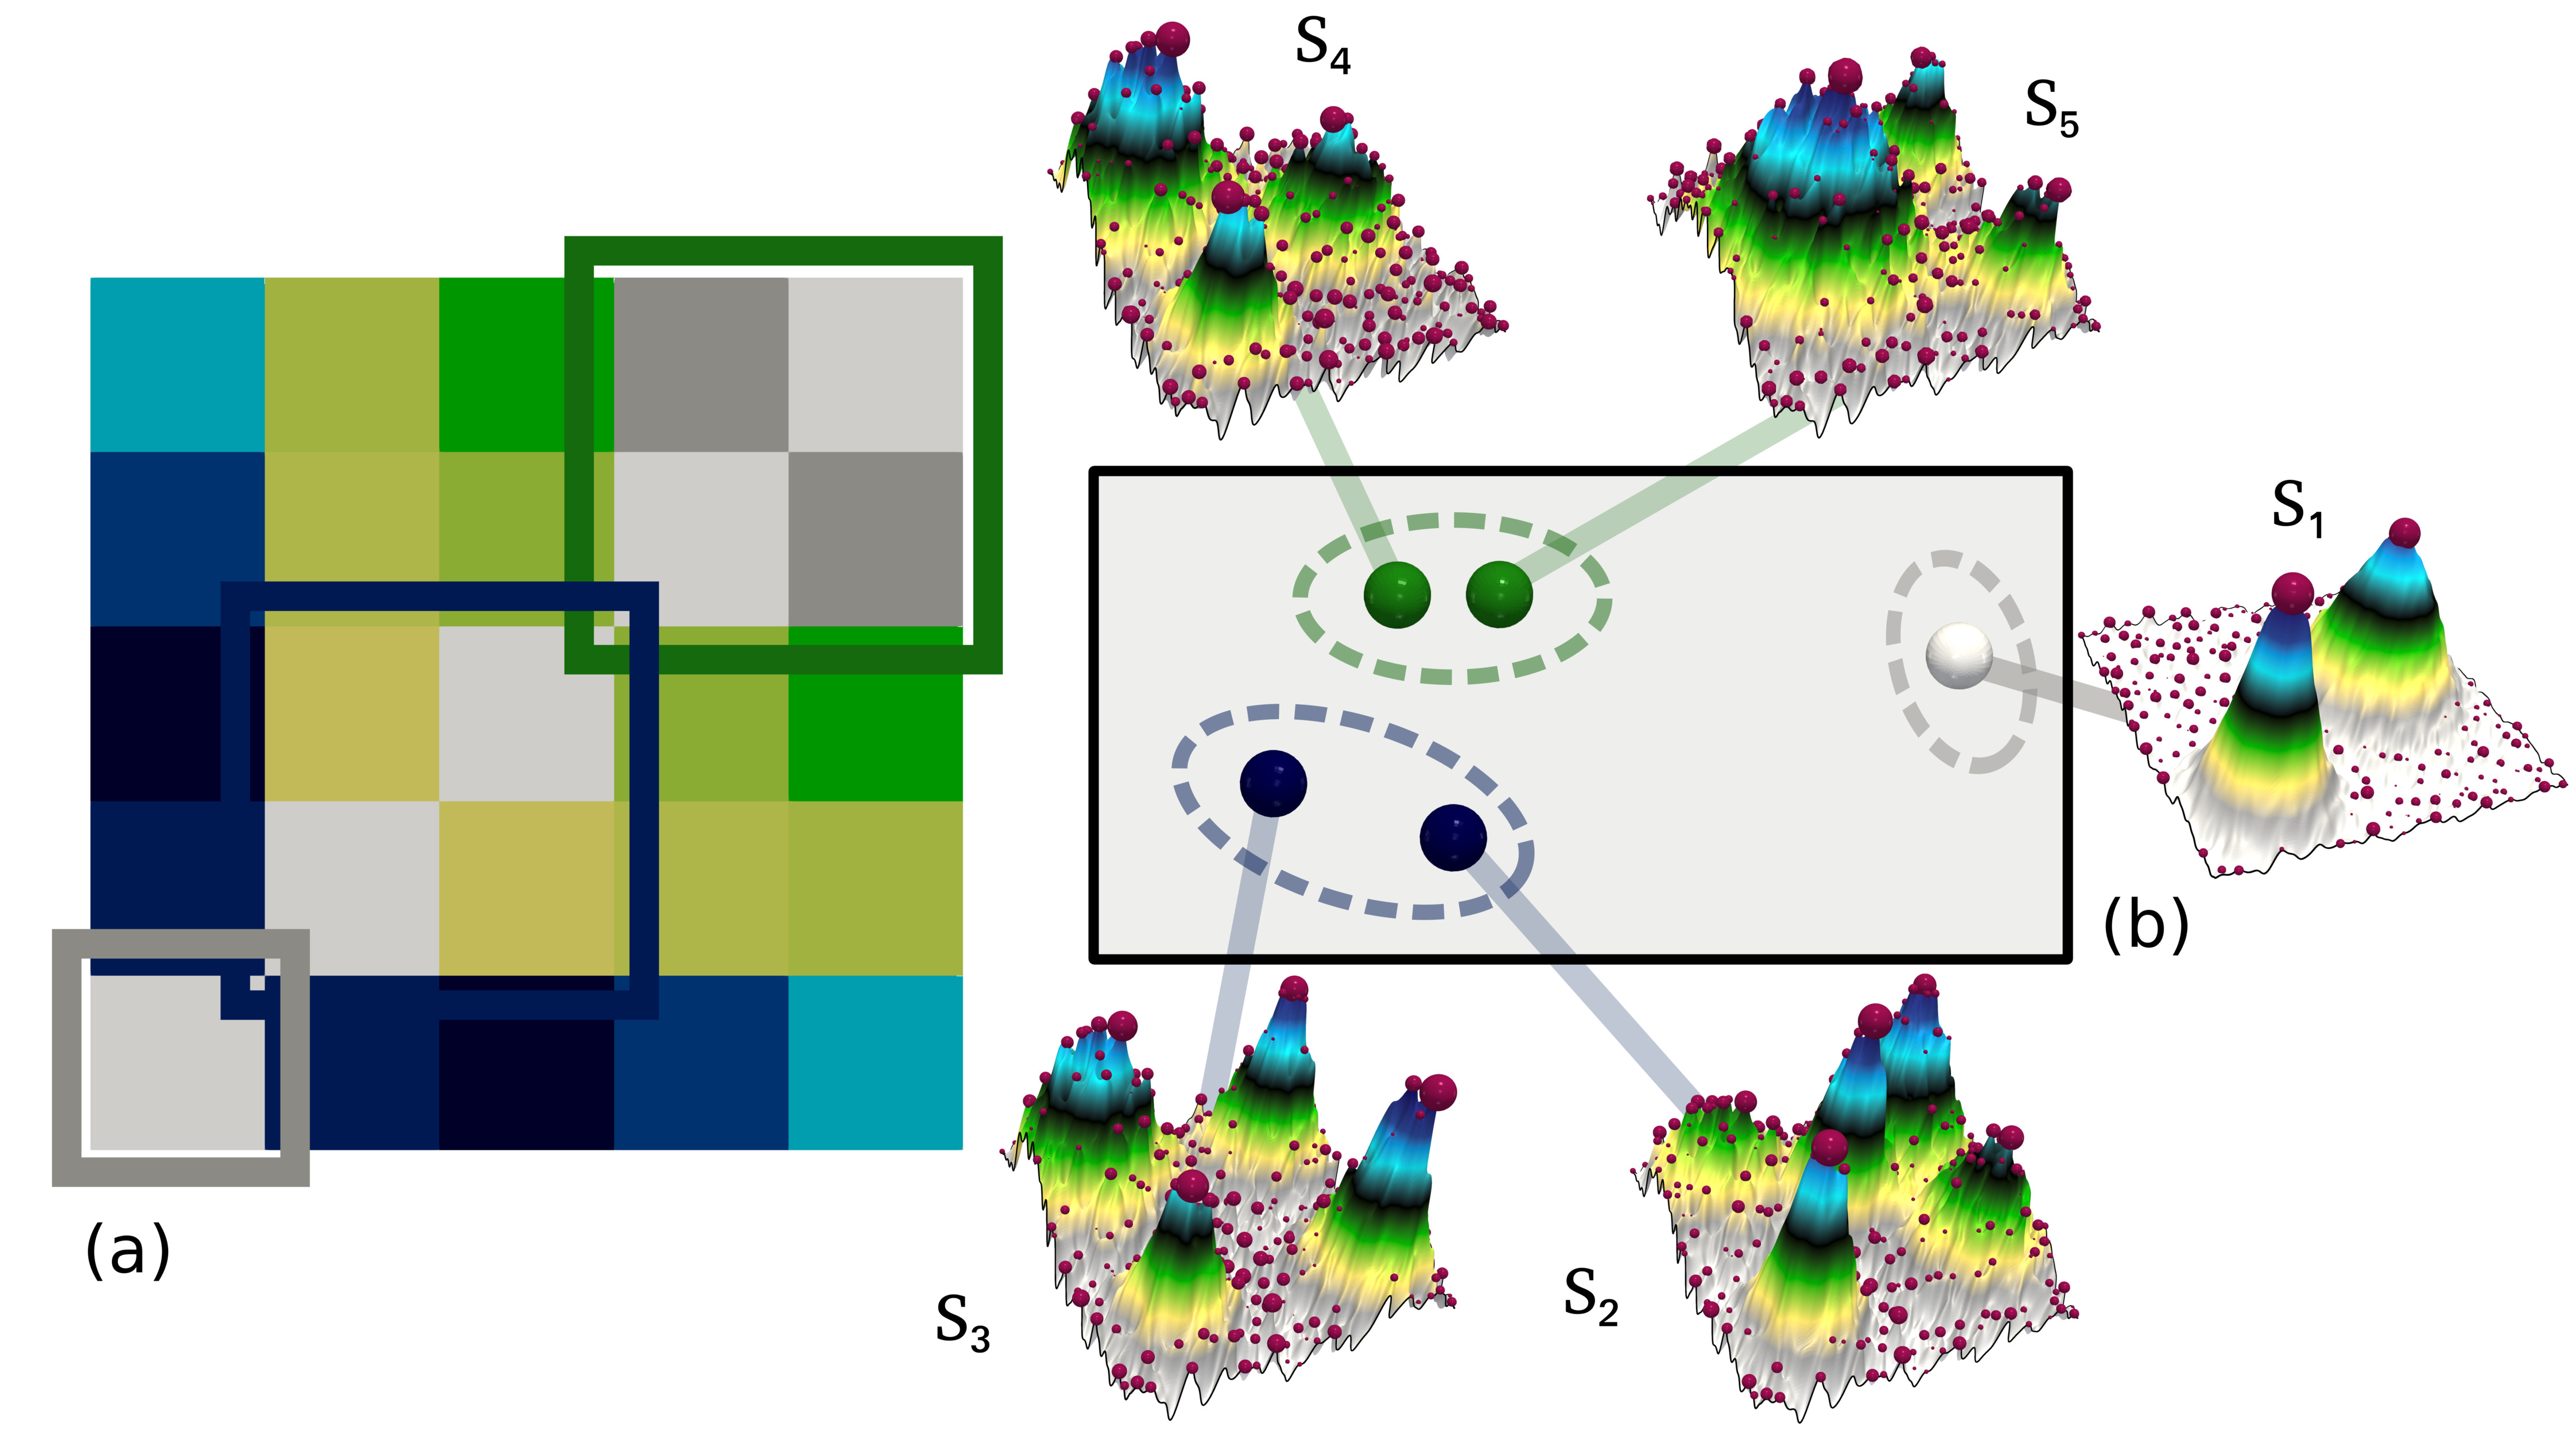
\includegraphics[width=\figureShrink\linewidth]{chapter4_topology_data_analysis/pictures/gaussian_cluster.jpg}
 \mycaption{
 Wasserstein distance matrix for five inputs $S_1$, $S_2$, $S_3$, $S_4$, $S_5$ generated respectively with two, five, for and three Gaussian
functions with different noise levels. Point cloud of the inputs in the Wasserstein distance space colored according to the clusters obtained with the k-means clustering method. We can see that each terrain in a cluster has the same number of Gaussian and level of noise.}
 \label{gaussian_cluster}
\end{figure}
\begin{figure*}
 \centering % avoid the use of \begin{center}...\end{center} and use \centering
 
\includegraphics[width=\figureShrink\linewidth]{chapter4_topology_data_analysis/pictures/KHI_courbes.jpg}
 \mycaption{
Schemes (left) and order (right) studies.
% , left orders study.
Average
persistence curves for 5 configurations with variations of : a (WENO-Z,5), c
(WENO-Z, 7), f (WENO-Z, 5), h (TENO,5). (b,g) persistence curves at $t_0$ (top),
$t_1$ (middle), $t_2$ (bottom).
 Vertical lines on the curves correspond to critical points of small (left) and
high (right) persistence.
% critical points (left) and high persistence (right).
(d,e) Integral differences (grey area) between average persistence curves for
all variations.}
\vspace{2ex}
 \label{curv}
\end{figure*}

\begin{figure*}
 \centering
 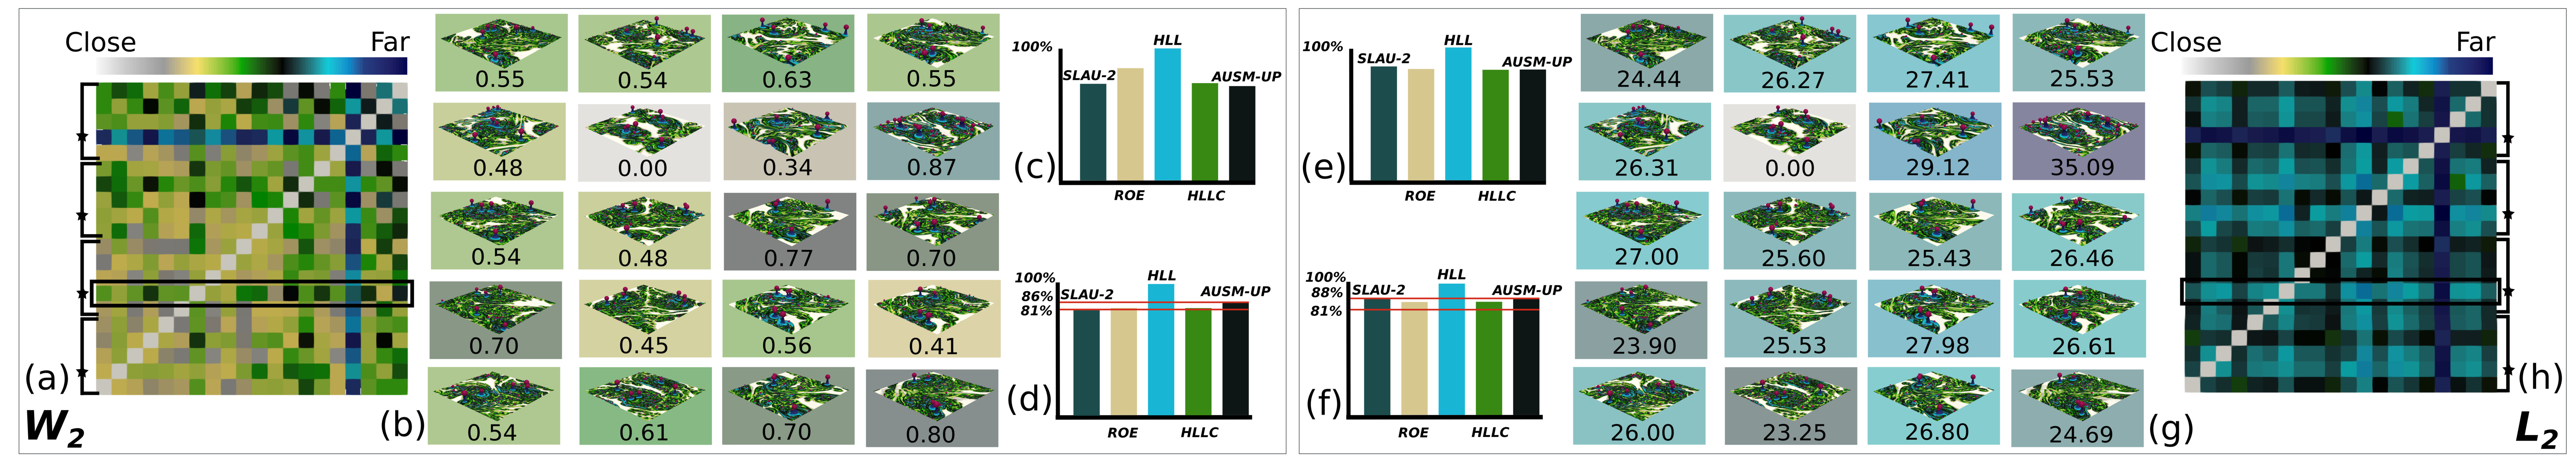
\includegraphics[width=\figureShrink\linewidth]{chapter4_topology_data_analysis/pictures/KHI_distance_to_the_rest.jpg}
 \mycaption{Comparison between the $\wasserstein{2}$ metric (left) and the standard $L_2$-metric (right) for isolating the HLL solver.
 (a,h) Distance matrix for 20 configurations at $t_2$ at $512 \times 512$. Black frames represent the distance between the TENO 7$_{th}$ order with the HLL (matrix lines marked by $\star$) and the other configurations (b,g). Histograms (c,e) are respectively the percentage average of the sum distance matrix of (a,h). Histograms (d,f) are respectively the percentage of the sum distance for all variations.}
 \label{fig_KHIdistance}
\end{figure*}


\subsection{Outlier distance profile}
\label{sec_outlier}
With this protocol (illustrated on toy examples,
\autoref{gaussian_distance}), we want to validate hypothesis H3 (\autoref{Hypotheses}), which means that for all the simulation configurations the HLL solver will be very different from other solvers to describe the Kelvin-Helmholtz instabilities. For this protocol, we take 5 simulation configurations where we fix the reconstruction (TENO or WENO-Z), the physical time ($t_0$, $t_1$, $t_2$), the mesh ($256\times 256, 512\times 512, 1024\times 1024$), the order (5 or 7) and we vary the solvers. The 5 different computations describing the same turbulent flow obtained with the solvers (HLL, SLAU2, AUSM$^+$-UP, HLLC and Roe) are analyzed regarding to the enstrophy.

A distance is used to compare the topology of the enstrophy. Many methods can be used to compute such a distance but in this protocol we focus on 2 metrics: the $L_2$-norm distance directly on the values of the enstrophy and the Wasserstein distance on the persistence diagrams. One can inject other distances if needed. For the Wasserstein, the saddle-maximum persistence diagram is computed on each result. Then, they are grouped in a unique dataset to compute a persistence diagram distance matrix (\autoref{gaussian_distance}). For the $L_2$-norm, a distance matrix  is also created where a line corresponds to the distance in the enstrophy field from one solver to the others.





Thus, the sum of the distances from one solver to the others is computed by
summing the distances on one line of the matrix. The total distance of one 
solver to the others, for all configurations, is simply the sum of all these sum 
distances for every line of the matrix which correspond to the same solver. We 
finally obtain one global distance per solver for all configurations. Finally 
the difference between the distance of the HLL and the distance of the maximizer 
(the second value if HLL is the maximum) gives a separation score. If the
difference is positive, then hypothesis H3 is verified whereas it is not if 
negative, because it means that another solver generates a flow topologically 
more different than the HLL. 
With this protocol, best separations are obtained for high absolute values.
% of 
% the score.

% the higher is the absolute value of the score, the 
% better the separation is.
% with this protocol.



\subsection{Unsupervised classification}
\label{sec_unsupervised}


With the last protocol (illustrated on toy examples in \autoref{gaussian_cluster}),
we want to validate hypotheses H4 and H5 (\autoref{Hypotheses}). We want to verify that the
simulations with the Roe and HLLC solvers are topologically close (hypothesis H4) and the
simulations with the AUSM$^+$-UP and SLAU2 solvers are topologically close (hypothesis H5). To do so, three clustering methods will be used based on Wasserstein distances and the L$_2$- norm(\autoref{sec_topology}).

For the first two clustering methods, we start by computing distance matrix with the protocol of the outlier distance profile \autoref{sec_outlier} using successively the Wasserstein distance and $L_2$-norm matrices (\autoref{gaussian_cluster}a). We apply a dimension reduction to project the distances of the matrix according to 2 components (\autoref{sec_topology}). This projection is used to generate clusters of the matrices with a k-means algorithm (\autoref{sec_topology}) as illustrated on \autoref{gaussian_cluster}b. The third clustering method uses directly the persistence diagrams(\autoref{sec_topology}) without using the distance matrix. All the persistence diagrams are merge into a single dataset to compute the Wasserstein distances between each diagram. The barycenter of persistence diagram is then used to directly compute a cluster, without dimension reduction, in the Wasserstein metric space \cite{vidal_vis19} with the ${W_2}$ distance. Then a k-means algorithm (\autoref{sec_topology}) is applied. 

With these three classification methods, we obtain different associations of our configurations. Each association is going to be scored with a measure of similarities between the clusters regarding to a reference cluster using the Rand Index \cite{rand1971objective}. This Rand index has a value between 0 and 1, with 0 indicating that two clusters do not agree on any pair of points and 1 indicating that the data clusters are exactly the same. Based on the properties of the solvers used in the simulation code HYPERION and detailed in \autoref{sec_solvers}, we define our reference cluster such that the first partition contains the AUSM$^+$-UP and SLAU2 solvers, the second partition the HLLC and Roe solvers and the third partition the HLL solver. The Rand Index is computed for each configuration and averaged per clustering method.
This
% metric
enables the
% precise
ranking of
% allows us to precisely rank
the different solver
behaviors.
% of our solvers.
If the average Rand Index score is close to 1 then both hypotheses H4, showing similarity between the AUSM$^+$-UP and SLAU2 solvers and H5, showing the isolation of the HLL solver, are verified.













\section{Results}
\label{sec_experimentalResults}
This section presents our experimental results and their interpretations, for
the protocols presented in \autoref{sec_protocols}, applied on the ensemble data
described in \autoref{sec_caseStudy}
% , which has been made
(publicly
available \cite{data}).


\subsection{Persistence curve study}



We applied protocol 1 using the persistence curves, on our ensemble dataset of Kelvin-Helmotlz instability (KHI) to verify the hypotheses of separation of the schemes (H1) and the independence of the orders (H2)(\autoref{Hypotheses}). 
The input parameters are setup as detailed in \autoref{sec_protocols}, generating 36 studies. The terrains and curves on
% Figure
\autoref{curv} illustrate the result for one configuration with a 5th order WENO-Z (\autoref{curv}.a), a 7th order WENO-Z (\autoref{curv}.c), a 5th order WENO-Z (\autoref{curv}.f) and a 5th order TENO (\autoref{curv}.h). For the scheme comparison, most of the averaged persistence curves for the TENO schemes (blue curves on \autoref{curv}g) are above the WENO-Z curves (green curves on \autoref{curv}g).
The integral difference, between the average curves, obtain results between $[-5.6,5.2]$ (\autoref{curv}.e), which demonstrates differences on the topology of the enstrophy between the interpolation methods as expected.
Hypothesis H1 is verified on the KHI ensemble dataset. For the study on the 
independence of orders, we see that the averaged persistence curves are often 
close (\autoref{curv}b). However the integral differences obtained for this 
study show larger values for the WENO-Z, \emph{i.e} in between $[-0.5, 8.1]$ 
(\autoref{curv}.d). This analysis highlights that orders play a more important 
role, in terms of topology of the vortices, for WENO-Z than for TENO. Moreover, 
we observe that this difference tends to increase at $t_2$ for both studies 
confirming that the flow is composed of a larger number of vortex as the 
simulation evolves. Hypothesis H2 is verified for the TENO solvers but not for 
the WENO-Z
% as discussed
% later 
% in
(\autoref{insights}).
 



\subsection{Outlier distance profile study}
\label{sec_KHIdistance}


% In order t
To verify the HLL isolation states in hypothesis H3 (\autoref{Hypotheses}) on our ensemble dataset, we implemented our protocol 2 (\autoref{sec_protocols}) based on the Wasserstein distance and the $L_2$-norm (\autoref{sec_topology}). For this study we apply protocol 2 where the time and the resolution are fixed. The parameters that vary are the schemes ($\times 2$), the orders ($\times 2$) and the solvers ($\times 5$) (\autoref{tab_parameters}) thus generating 20 cases. All the distances have been computed according to the protocol of the outlier distance profile. These distances are represented by a global distance matrix where a line represents the 20 configurations (Wasserstein \autoref{fig_KHIdistance}.a and $L_2-$norm \autoref{fig_KHIdistance}.h) compared to a the HLL solver choosen as the reference. The matrix view of \autoref{fig_KHIdistance}b and \autoref{fig_KHIdistance}g show the KHI terrains and the distances of all configurations to the HLL solver.

The study has been done for all time steps and all resolutions generating nine
$20\times 20$ 
distance matrices, for each distance. The histograms (Figs. 
\ref{fig_KHIdistance}.c and \ref{fig_KHIdistance}.e) 
% (\autoref{fig_KHIdistance}.c) and (\autoref{fig_KHIdistance}.e) 
show the average 
of these nine distance matrices for the Wasserstein distance and the 
$L_2$-norm, expressed in terms of percentage according to the distance of HLL 
to the other solvers (HLL being the reference at 100\%). In this case the 
percentage difference in distances to HLL are about 18\% 
(\autoref{fig_KHIdistance}.d) for the Wasserstein and 13\% for the $L_2$ 
(\autoref{fig_KHIdistance}.f). These large percentages confirm that HLL is a 
solver that behaves differently from others.
% More precisely, a
As it does not take
into account contact discontinuities, the interfaces between the vortices
are much less defined than with the other solvers, resulting in a different
number of vortices. From a physical point of view, this result confirms the 
isolation of HLL in all cases. From a topological point of view, it shows that 
the Wasserstein distance is the best at differentiating the HLL solver from the 
others (the distance gap is always bigger than the $L_2$). For this large study 
of 18 distance matrices $20\times 20$, the hypothesis H3 is verified. 

\begin{figure*}
 \centering % avoid the use of \begin{center}...\end{center} and use \centering
 \vspace{-1ex}
 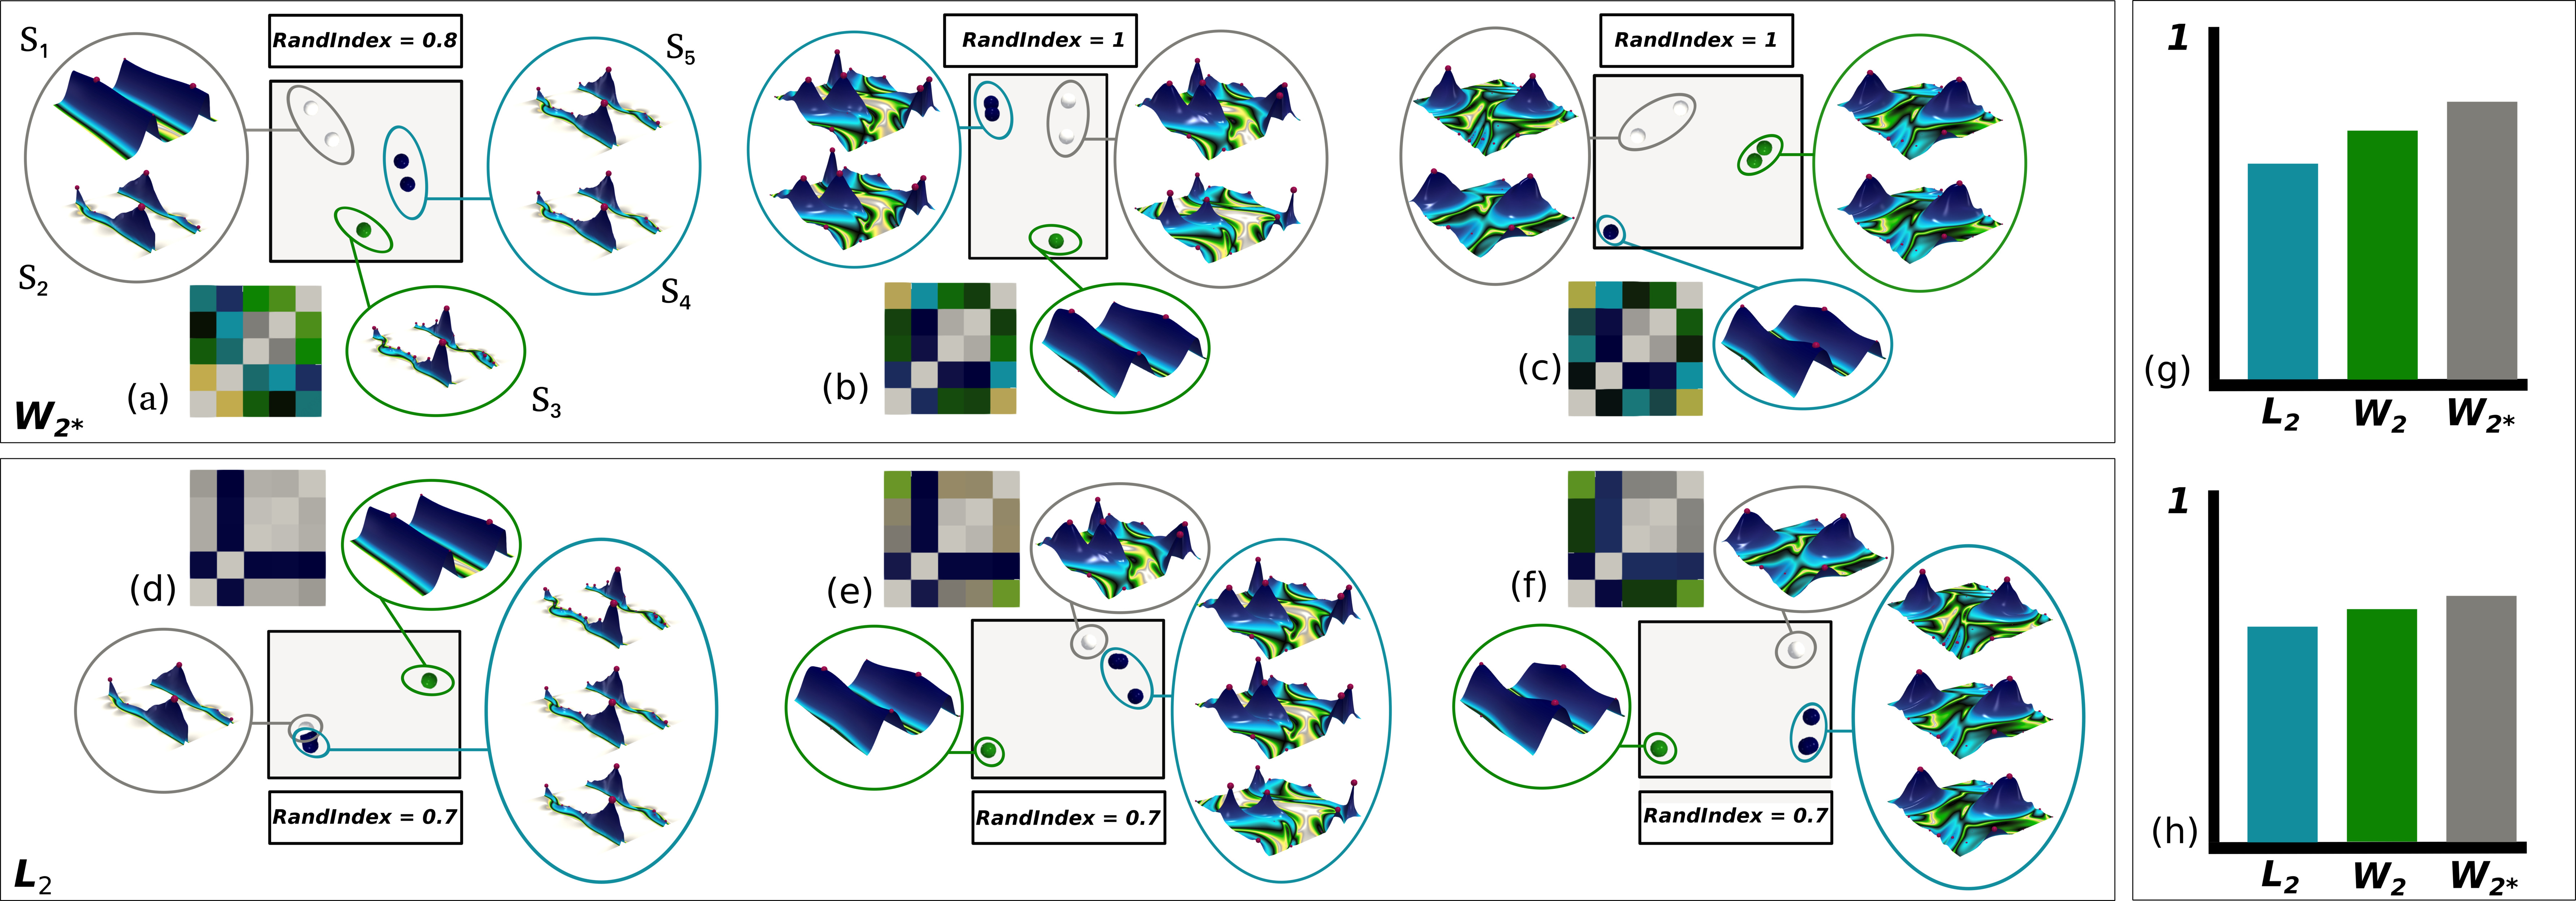
\includegraphics[width=\figureShrink\linewidth]{chapter4_topology_data_analysis/pictures/KHI_cluster.jpg}
 \mycaption{Comparison between the clustering on the Wasserstein metric space \cite{vidal_vis19} (top frame) and a clustering based on the traditional $L_2$ norm (bottom frame) for distinguishing FDS solvers from FTS solvers.
Point clouds at $t_0$, $t_1$,$t_2$ with a first order scheme at $256\times 256$.
The point cloud is a representation of the five scalar-fields in the distance
space colored according to the clusters obtained. The Rand Index are computed
with the five configurations $S_1$ (SLAU2), $S_2$ (HLL), $S_3$ (AUSM$^+$-UP),
$S_4$ (Roe), $S_5$ (HLLC). (g,h) Average Rand Index for all variations for the
high orders (bottom) and the first order (top).}
\label{fig_khi_cluster}
\end{figure*}


\subsection{Unsupervised classification study}
 \label{sec_khi_cluster}
To improve our understanding on the behavior of the solvers into our simulation code, we implemented protocol 3 on the unsupervised classification (\autoref{sec_protocols}) to verified the hypotheses H4 and H5 (\autoref{Hypotheses}). The goal is to identify the separation of FDS type solvers from the FTS type solvers (\autoref{sec_solvers}). We are interested in the low Mach reconstructions (\autoref{sec_solvers}). The challenge comes from the fact that small vortices are reconstructed on only a few cells. So, we implemented protocol 3 with the distances and clustering method detailed in \autoref{sec_protocols} leading to 5 simulation configurations (\autoref{tab_parameters}) with variable solvers. To focus on the small vortices we used a threshold of 0.38 persistence for the topological methods. On the KHI ensemble, we generated 36 clusters from the threshold persistence diagrams and obtain the Rand Index for all of them. \autoref{fig_khi_cluster}.a, \autoref{fig_khi_cluster}.b, \autoref{fig_khi_cluster}.c show the $W_2*$ clustering for the three timesteps and \autoref{fig_khi_cluster}.d, \autoref{fig_khi_cluster}.e, \autoref{fig_khi_cluster}.f for the $L_2$.

Histogram \autoref{fig_khi_cluster}.h shows the average Rand Index for the 
three methods with a value of 0.63 for $L_2$, 0.66 for $W_2$ and 0.71 for $W_2*$.
There is very little difference between the topological and geometric results 
and each of the methods struggles to get the right cluster. Hypotheses H4 and H5 
are not verified for high orders. However, to highlight the differences between 
solvers, it is necessary to use a reference reconstruction that barely captures 
small scale turbulence due to order dissipation (\autoref{sec_solvers}).
Thus, we applied protocol 3 (\autoref{sec_protocols}) on a more restricted 
dataset at order 1. Histogram \autoref{fig_khi_cluster}.g shows the average 
Rand 
Index at order 1 with the three methods leading to 0.63 for $L_2$, 0.71 for $W_2$
and 0.78 for $W_2*$. In this case, we notice that for any reconstruction, the 
topological methods obtain better clustering. Moreover, the study with order 1 
shows that the $W_2*$ method enhances solver isolation.
% of the solvers.
With this
high score of the Rand Index hypotheses H4 and H5 are verified with the first 
order. 

\subsection{Unanticipated insights}
\label{insights}

During the analysis of the persistence curves generated by our protocol 1, we found significant differences on the topology of the enstrophy between the orders for the WENO-Z. By increasing the order, we increase the accuracy of our calculation that generates more structures into the turbulent flow. On the other hand, there is no difference between the orders obtained with the TENO. This means that other ingredients in the TENO reconstruction play an important role in the computation of the turbulence such as the separation of the scales. In addition, the persistence curves also allowed us to observe that the WENO-Z schemes produce more numerical errors than the TENO. As presented in \autoref{sec_khi_cluster}, H4 and H5 hypotheses have not been verified for high orders. This means that the topological analysis does not capture the differences between the solvers. This may be due to the reconstructions which are accurate enough to calculate all velocities in the Kelvin-Helmholtz instability. 

\subsection{Limitations}
As discussed in \autoref{sec_KHIdistance}, in comparison to the $L_2$ norm, the Wasserstein distance
improvesthe separation of the HLL solver, but only by $5 \%$ (distance difference percentage). While this improvement may seem marginal, we would like to stress its significance given such challenging data,in particular with regard to the traditional approach based on kinetic energy, shown \autoref{energie}, where the five solvers can hardly be distinguished from each other.

Similarly, we can see that the Rand Index score for the three clustering
methods detailed in \autoref{sec_khi_cluster} are quite close to each other as
illustrated on \autoref{fig_khi_cluster}.h. These close scores are due to the 
interpolations schemes (\autoref{sec_simulation}) which cover up the differences 
between the different solvers.
In other words, the variations in vortex distributions induced by the choice of solver are too subtle, given the importance of the interpolation order on the outcome. As shown in \autoref{fig_khi_cluster} (top), we were still able to overcome this limitation by considering a
reconstruction that is not dedicated to turbulence, \emph{i.e.} an upwind scheme 
of order 1. This enabled us to exaggerate the impact of the solvers, thereby allowing us to
validate hypotheses H4 and H5 as reported in \autoref{sec_khi_cluster}.


\section{Conclusion}
In this paper, we have presented an experimental protocol for the comparison of
numerical methods on a Kelvin-Helmholtz instability using topological analysis.
An ensemble dataset of 180 members has been computed for this instability by a
simulation code developed in our institution and running on a supercomputer.
While traditional approaches based on the kinetic energy (\autoref{energie}) only enable
to validate the physical conformity of the generated flow,
% to assess the physical conformity of the generated flow,
our overall approach provides finer analyses. In particular,
% Based on the assumptions made in the literature (\autoref{sec_simulation}),
the
protocol using the persistence curves (\autoref{sec_persistence}) allowed us to
observe differences between the TENO and WENO-Z reconstructions. It also
confirms an independence of the
reconstruction order (5 or 7) when
using the TENO scheme allowing
% speedup
practical
computational speedup,
without loss of precision. The protocol
based on the Wasserstein distance (\autoref{sec_outlier}) succeeded in
discriminating the HLL solvers from other configurations, validating the use of
such a topological analysis to confirm domain field expectations. The last
protocol, based on recent clustering methods (\autoref{sec_khi_cluster})
successfully differentiates the topology of computations based on FDS (Flux
Difference Splitting) and FTS (Flux Type Splitting) solvers.
Overall, the validation of the hypotheses reported by CFD experts (\autoref{sec_hypotheses}) provides reliable indications for the tuning of a flow simulation, to help CFD users achieve the best balance between computation accuracy and speed.
%
%
% in contrast to traditional approaches (\autoref{energie}), which only validate the physical plausibility of a flow, our framework enabled the validation of the above hypotheses (formalized in \autoref{sec_hypotheses})}
% In particular, the validation of these hypotheses are a practical contribution towards }
% Flux Differe
% (FDS) and FTS solver computations.


The results obtained in this experimental study also show
the viability of topological methods for the representation and comparison of
Kelvin-Helmholtz
instabilities.
%
% that
%
% we can take confidence in the topological treatment for a Kelvin-Helmholtz
% instability.
The interesting aspect of these topological protocols is that the
numerical method comparisons are based on physical differences rather than on
unreliable, low-level, pointwise measures.
% quantitative.
The direction we wish to take now, for our future work, is
the extension of these protocols to 3D datasets of external hypersonics aerodynamics.
% However, in order to isolate one phenomenon on 3D data, a
% threshold study will have to be implemented. It will be necessary to decide
% which phenomenon we want to observe, such as boundary layer turbulence or
% vortices generated at the back of the hypersonic vehicle.
Another direction we
want to investigate is the evaluation of other tools used in the protocol such
as new topological distances \cite{pont_vis21} or clustering methods. Finally, this experimental
study allows us, with confidence, to consider applying these protocols to other
hydrodynamic turbulent flows studied in our institution in the domain of
hypersonic vehicle design.


% \section{Acknowledgments}
%future work:
%benchmark for other topological comparison methods.


\chapter{Méthode numérique du code Hyperion en 3D}

\minitoc
\thispagestyle{empty}
\newpage

\chapter{Wall model adapted to hypersonic flow and IBM}

\begin{figure}[!ht]
 \centering
 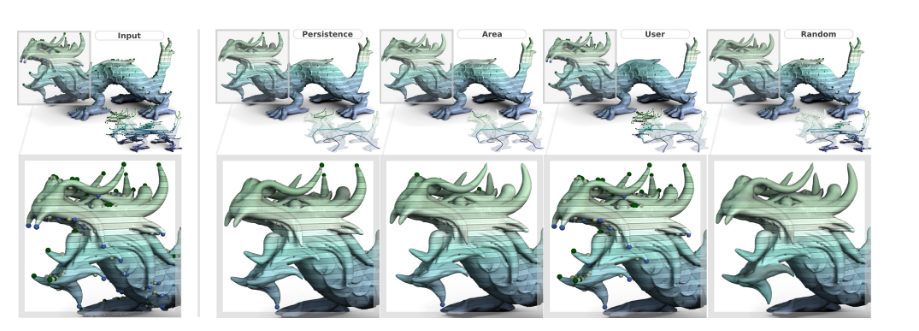
\includegraphics[width=1\linewidth]{chapter4_topology_data_analysis/pictures/picture_chapter.png}
 \vspace{-2ex}
 \caption{IXV spatial navette by esa}
  \vspace{2ex}
 \label{11}
\end{figure}
\minitoc
\thispagestyle{empty}
\newpage

\section{Comportment d'une couche limlite}
\subsection{Equation d'une couche Limite et description}
\subsection{Pourquoi utilisé une loi de paroi}

\section{introduction à la modelisation de paroi}
\subsection{Modélisation à la paroi}
\subsection{modele algebrique}
\subsection{modele TBLE}
\subsection{Modele pour LES}
\subsection{Limitations LES}

\section{Implémentation du modele da paroi dans hyperion}
\subsection{Modele choisi}
\subsection{Implémentaion des conditions limites}
\subsection{Implémentation de la methode avec les sondes}


\section{Résultats 2D}
\section{Résultat 3D}


\bibliographystyle{plain}
\bibliography{bib.bib}
\end{document}
